\section{RCS from Local Coins}
\label{app:Local Coin}

\begin{algorithm}[h]
\SetAlgoLined
\KwIn{
Number of models $|\mathcal{MG}|=n$; number of safe models $s$; 
round $R$; distributions $p_1, \ldots, p_n \in \mathrm{Distr}(\mathcal{Y})^{n}$
}
\KwOut{Response $y \in \mathcal{Y}$}

$Buffer \gets \varnothing$\\
\For{$r \leftarrow 1$ \KwTo $R$}{
    Sample $y \sim \frac{1}{n}\sum_{i=1}^{n} p_i$ \\
    $\sigma(y) =\frac{\frac{1}{s}\sum_{i=1}^{s} p_{(i)}(y)}
             {\frac{1}{n}\sum_{i=1}^{n} p_i(y)}$
        
    \If{accept $y$ with $\sigma(y)$}{
        \Return $y$
    }
    $Buffer \gets Buffer \cup \{\langle y, \sigma(y) \rangle \}$\\
}
$c \gets Random()$ \textcolor{mGreen}{\#Obtain local coin 0 or 1.} \\
\If{$c==0$}{
\Return $\bot$
}\Else{

Sort $Buffer=\{\langle y_i, \sigma(y_i) \rangle \}_{i=1}^{R}$ 
 such that $\sigma(y_{(1)}) \ge \dots \ge \sigma(y_{(R)})$\\
Let $\mathcal{F} = \{y_{(1)}, \dots, y_{u}\}, \; u= min(s,R)$ \\
\For{$i \leftarrow 1$ \KwTo $u$}{
    $\alpha(y_{(i)}) = \sum_{j=s+1}^{n} p_{(j)}(y_{(i)})$
}
\Return $y \gets \arg\max_{y \in \mathcal{F}} \alpha(y)$

}


\caption{Reliable Consensus Sampling from Local Coins}
\label{alg:coin}
\end{algorithm}



\section{Proof}
\label{app:ac}

\begin{align*}
&\sigma(y_t) - \sigma(y_v) \\
&=
\frac{\frac{1}{s} \sum_{i \le s} p_{(i)}(y_t)}
     {\frac{1}{n} \sum_{i=1}^{n} p_i(y_t)}
-
\frac{\frac{1}{s} \sum_{i \le s} p_{(i)}(y_v)}
     {\frac{1}{n} \sum_{i=1}^{n} p_i(y_v)}
\\[2mm]
&=
\frac{
\left( \frac{1}{s} \sum_{i \le s} p_{(i)}(y_t) \right)
\left( \frac{1}{n} \sum_{i=1}^{n} p_i(y_v) \right)
-
\left( \frac{1}{s} \sum_{i \le s} p_{(i)}(y_v) \right)
\left( \frac{1}{n} \sum_{i=1}^{n} p_i(y_t) \right)
}{
\left( \frac{1}{n} \sum_{i=1}^{n} p_i(y_t) \right)
\left( \frac{1}{n} \sum_{i=1}^{n} p_i(y_v) \right)
}
\\[2mm]
&=
\frac{n}{s} \cdot
\frac{
\left( \sum_{i \le s} p_{(i)}(y_t) \right)
\left( \sum_{i=1}^{n} p_i(y_v) \right)
-
\left( \sum_{i \le s} p_{(i)}(y_v) \right)
\left( \sum_{i=1}^{n} p_i(y_t) \right)
}{
\left( \sum_{i=1}^{n} p_i(y_t) \right)
\left( \sum_{i=1}^{n} p_i(y_v) \right)
}
\\[2mm]
% &=
% \frac{n}{s} \cdot
% \frac{
% \left( \sum_{i \le s} p_{(i)}(y_t) \right)
% \left(
% \sum_{i \le s} p_{(i)}(y_v)
% +
% \sum_{i > s} p_{(i)}(y_v)
% \right)
% -
% \left( \sum_{i \le s} p_{(i)}(y_v) \right)
% \left(
% \sum_{i \le s} p_{(i)}(y_t)
% +
% \sum_{i > s} p_{(i)}(y_t)
% \right)
% }{
% \left( \sum_{i=1}^{n} p_i(y_t) \right)
% \left( \sum_{i=1}^{n} p_i(y_v) \right)
% }
% \\[2mm]
&=
\frac{n}{s} \cdot
\frac{
\left( \sum_{i \le s} p_{(i)}(y_t) \right)
\left( \sum_{i > s} p_{(i)}(y_v) \right)
-
\left( \sum_{i \le s} p_{(i)}(y_v) \right)
\left( \sum_{i > s} p_{(i)}(y_t) \right)
}{
\left( \sum_{i=1}^{n} p_i(y_t) \right)
\left( \sum_{i=1}^{n} p_i(y_v) \right)
}
\end{align*}


\section{Additional Discussion}
\subsection{RCS and Multi-Agent Debate}

Multi-agent debate (MAD) \citep{du2024improving, chan2024chateval, liu2025breaking} is a reasoning enhancement technique built on LLM inference. MAD enables multiple agents to interact over several rounds. The goal is to encourage consensus on the same answer to a given query. A final decision is then produced through answer aggregation methods such as majority voting \citep{du2024improving}. In terms of output safety, MAD and RCS share a similar motivation. Both approaches introduce multiple models to improve the safety of the final output. Some MAD methods also adopt confidence scores to evaluate candidate answers proposed by other models \citep{chen-etal-2024-reconcile}. This mechanism is conceptually related to RCS. Compared to MAD, RCS follows a more fundamental strategy. RCS directly operates on underlying probability distributions. In contrast, MAD requires models to possess an explicit understanding of safety. This requirement limits robustness against unforeseen attacks. Moreover, RCS does not require interaction among models. This design avoids the conformity \citep{weng2025do} inherent in LLMs. Operating on underlying probability distributions also mitigates the impact of hallucination \citep{ji-etal-2023-towards} during reasoning. However, this design limits practical applicability. In many scenarios, models are accessed as black-box services, and probability distributions are not available. We argue that an intersection between MAD and RCS can improve the practical applicability of RCS. We continue to avoid direct interaction among models. Instead, each model outputs a score for each candidate output $y$ at every round. This score represents the level of support for $y$. All other components remain consistent with RCS. We refer to this variant as Practical Reliable Consensus Sampling (PRCS). More broadly, PRCS can be applied beyond safety. It can also enhance model reasoning performance in domains such as mathematics, medicine, and programming \citep{luo2025large}.

\section{Additional Experimental Results}
\label{app:results}
\begin{figure*}[h]
    \centering
    \begin{subfigure}{0.31\textwidth}
        \centering
        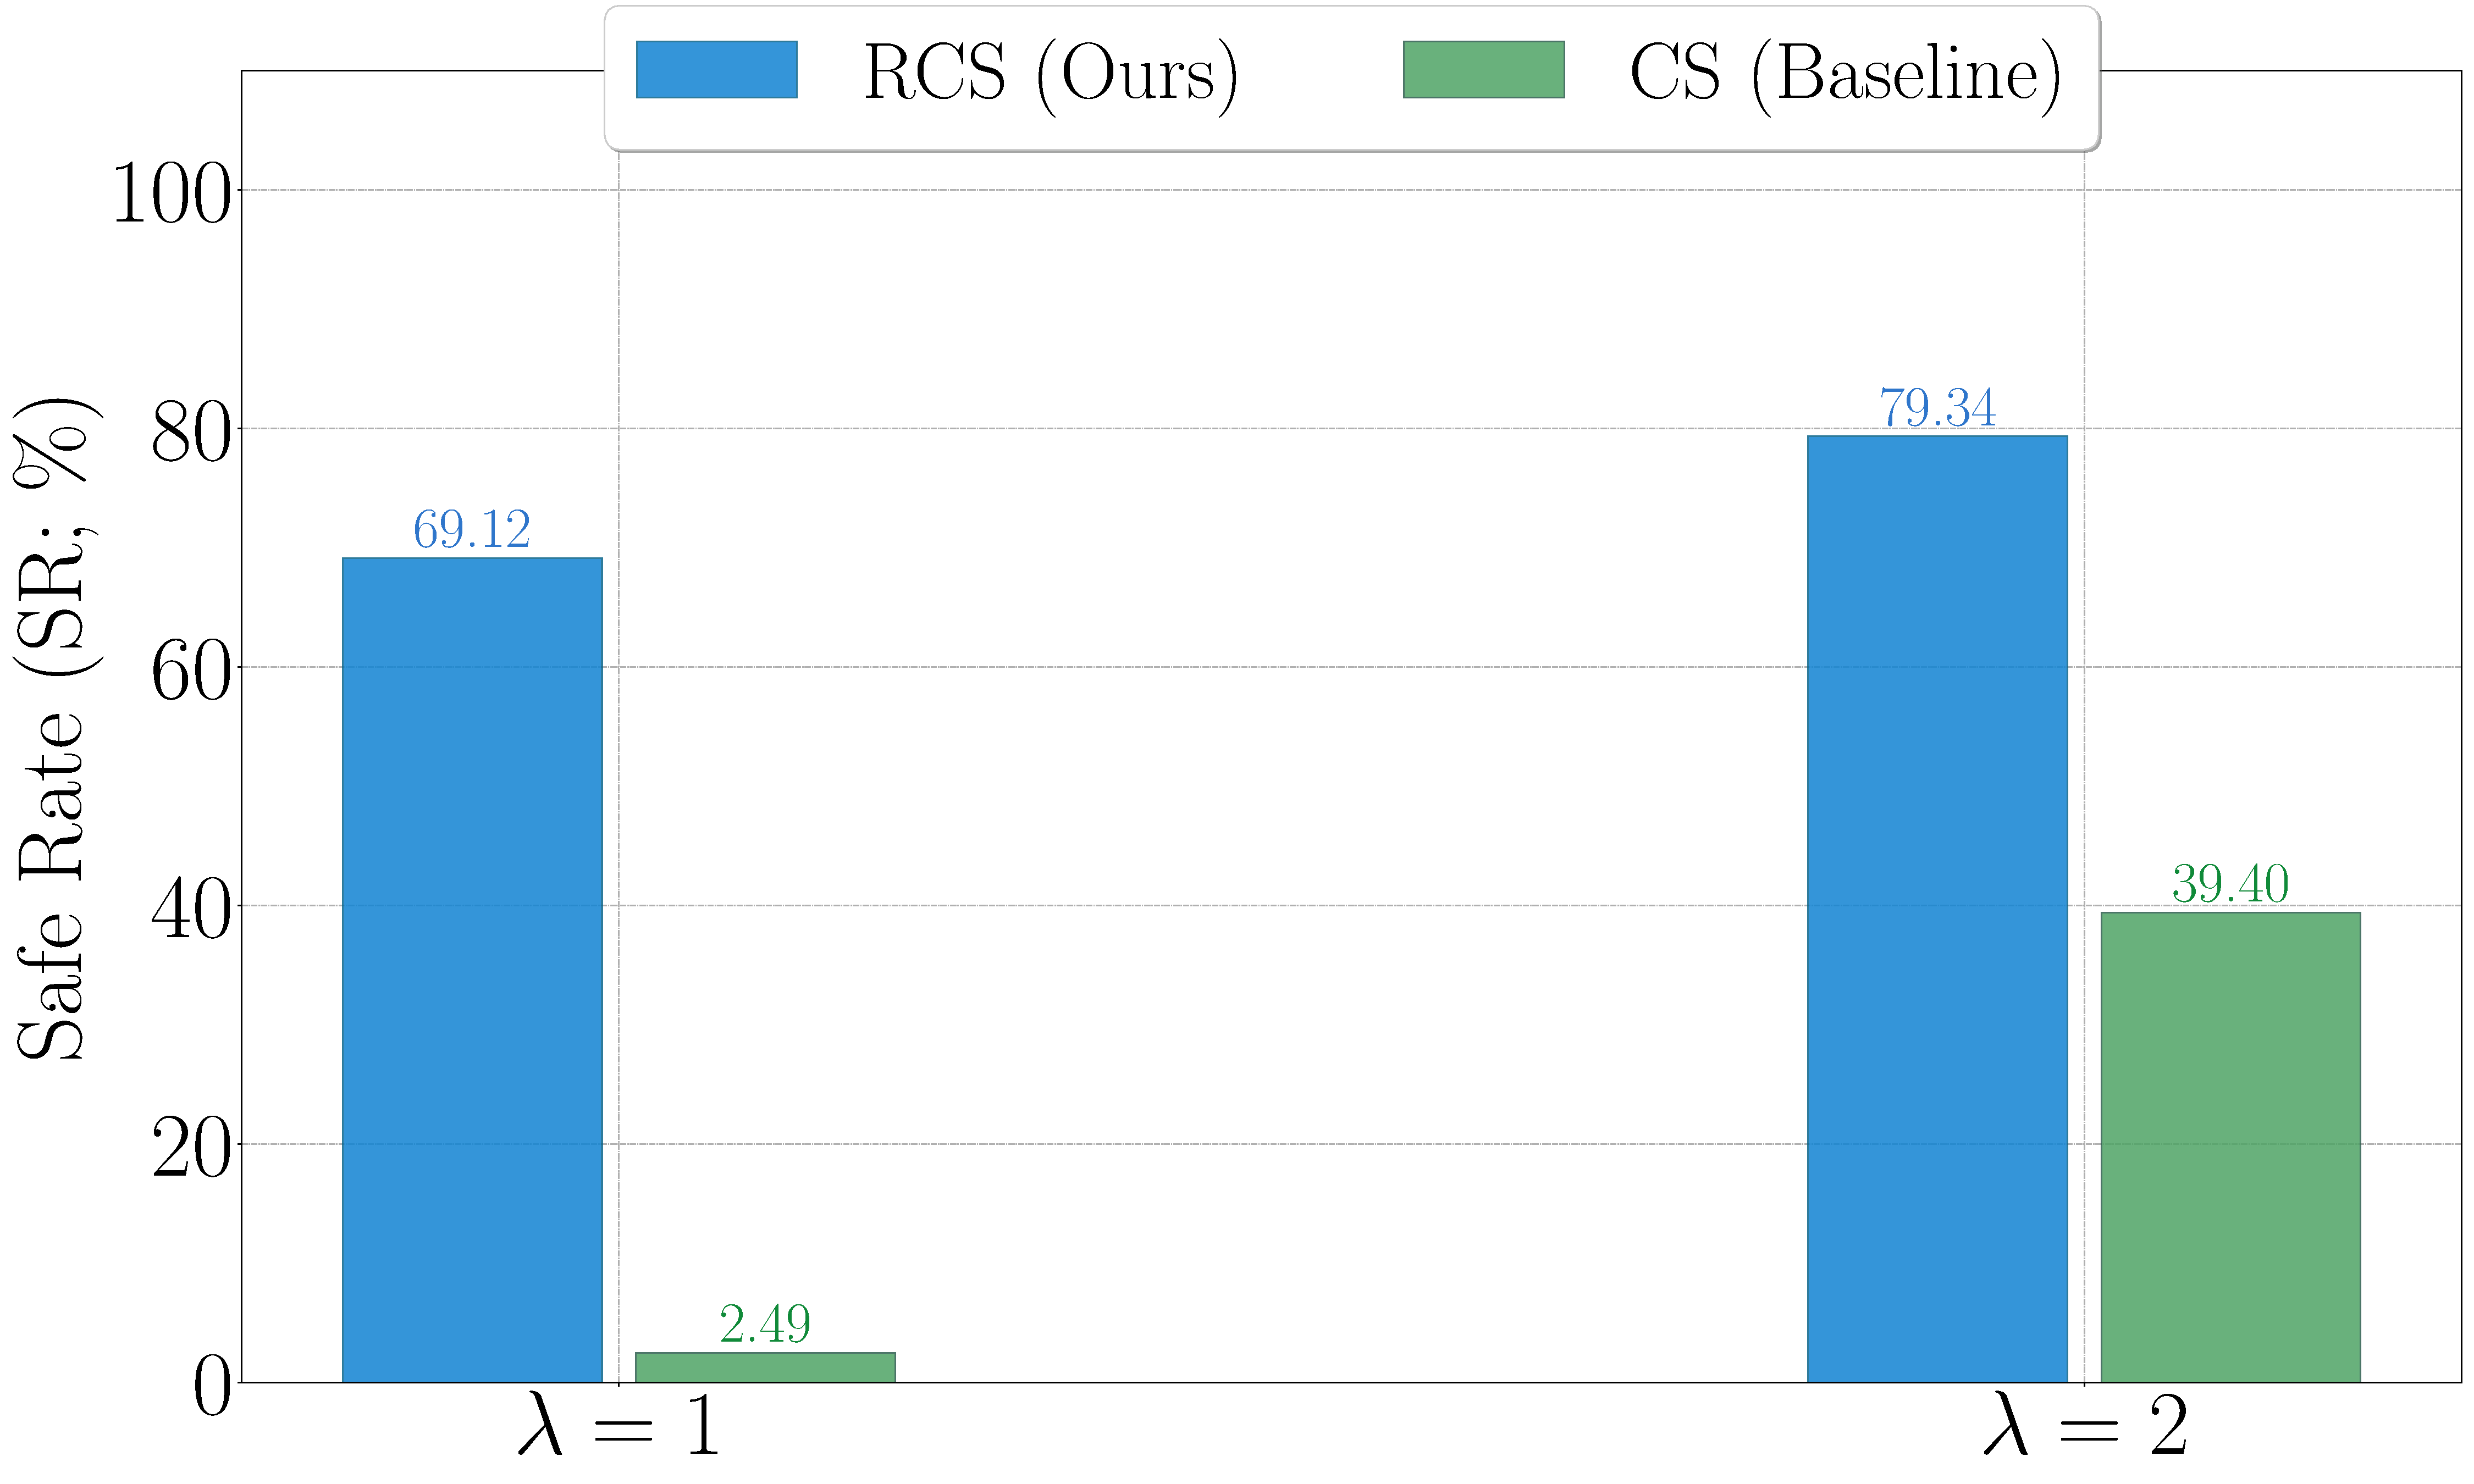
\includegraphics[width=\linewidth]{latex/eval_res/SR-5.pdf}
        \caption{$n=5$.}
    \end{subfigure}
    \begin{subfigure}{0.31\textwidth}
        \centering
        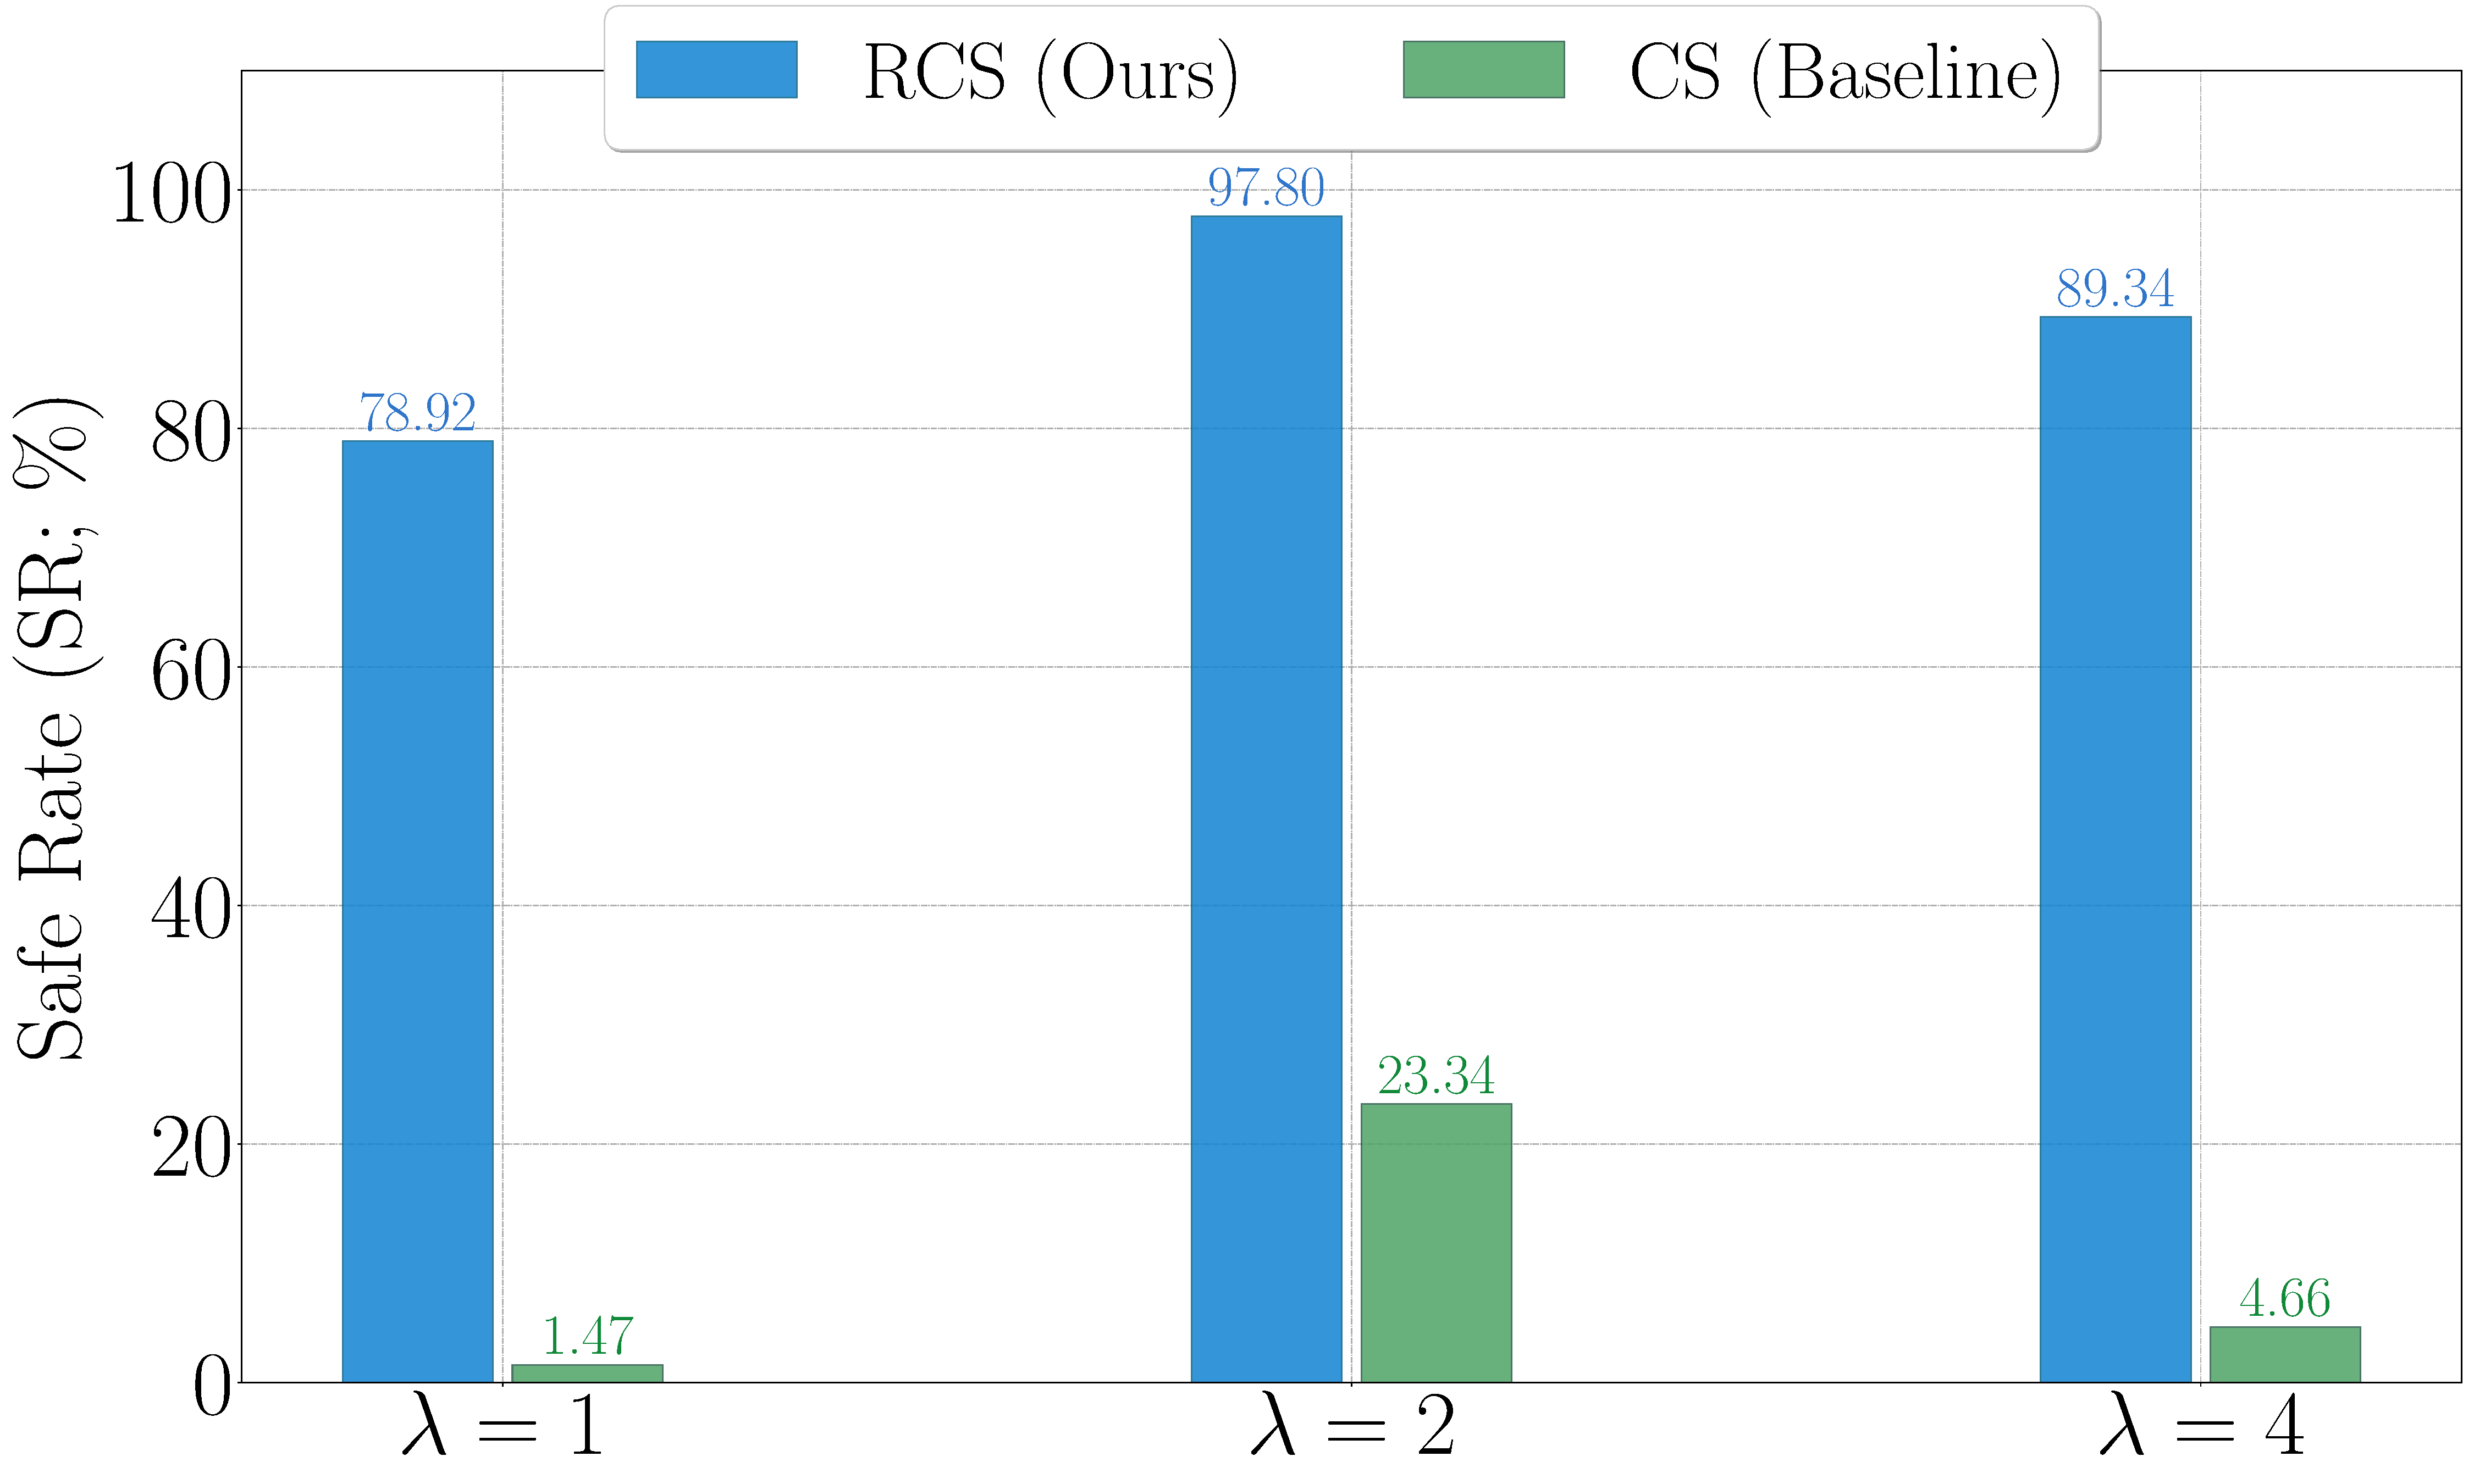
\includegraphics[width=\linewidth]{latex/eval_res/SR-9.pdf}
        \caption{$n=9$.}
    \end{subfigure}
    \begin{subfigure}{0.31\textwidth}
        \centering
        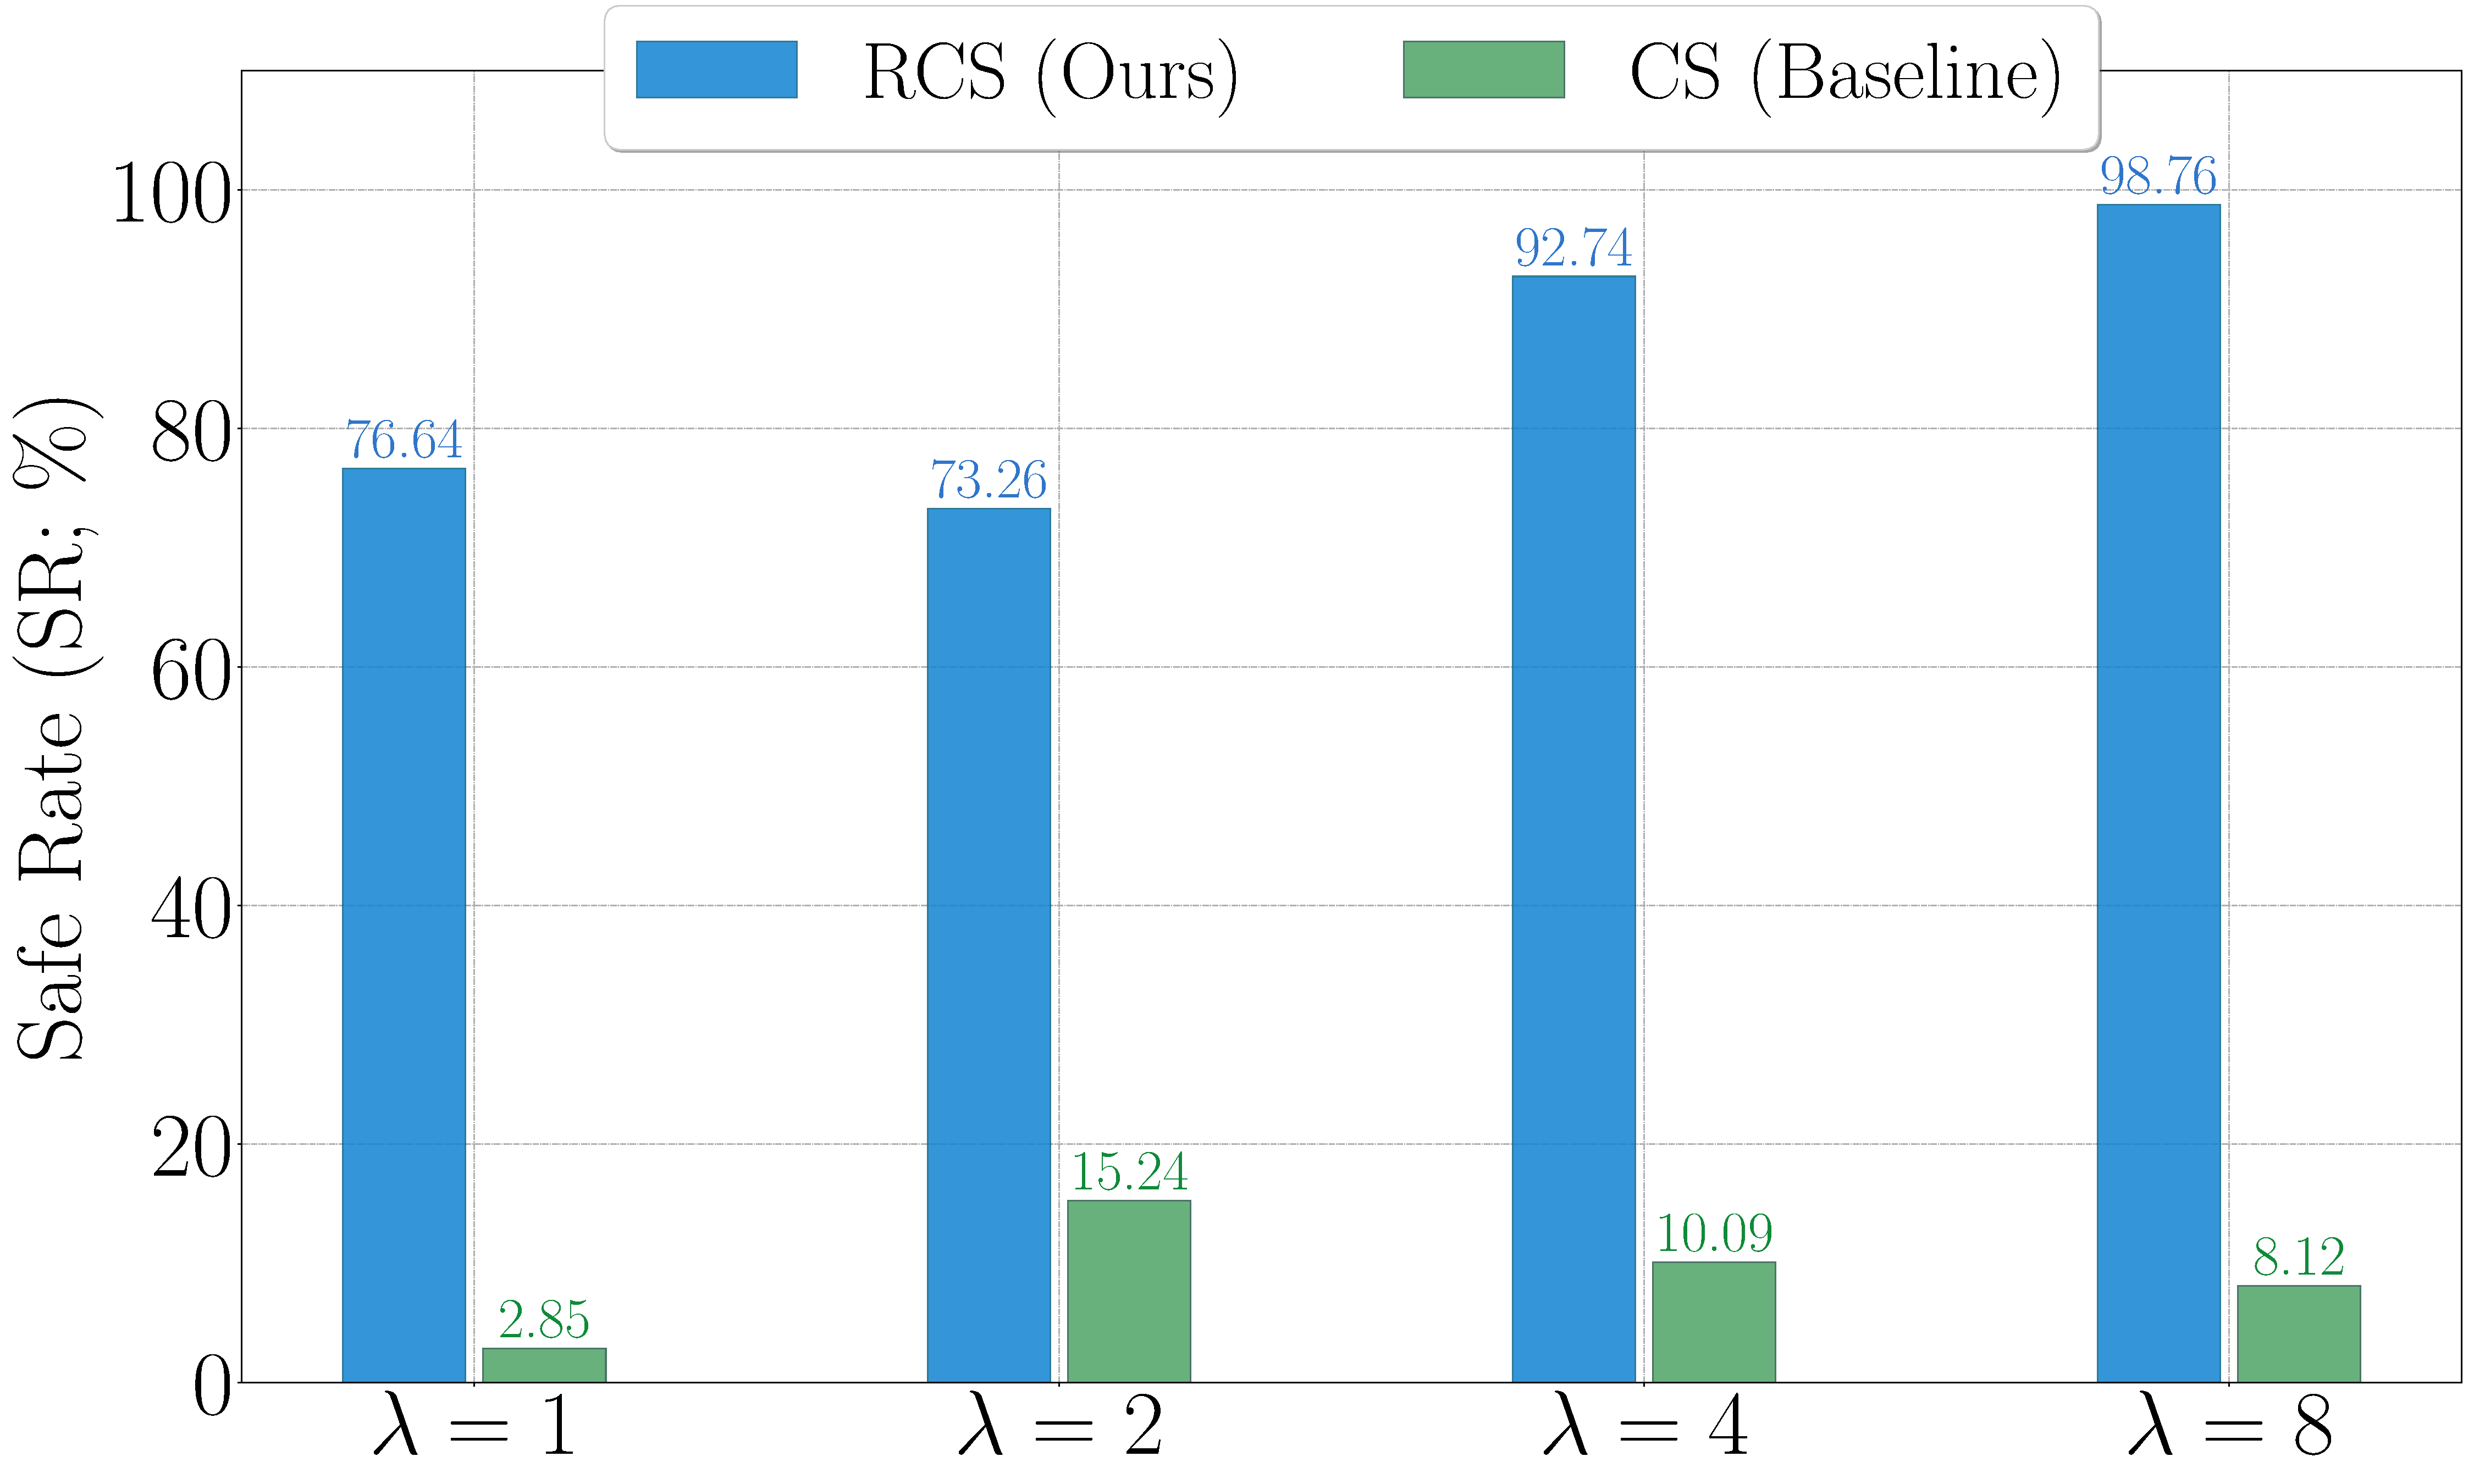
\includegraphics[width=\linewidth]{latex/eval_res/SR-17.pdf}
        \caption{$n=17$.}
    \end{subfigure}
    \caption{Evaluation results for the safe rate when $f < \lceil \frac{n}{2} \rceil$.}
    \label{fig:sr_app}
    \vspace{-15pt}
\end{figure*}


\begin{figure*}[h]
    \centering
    \begin{subfigure}{0.31\textwidth}
        \centering
        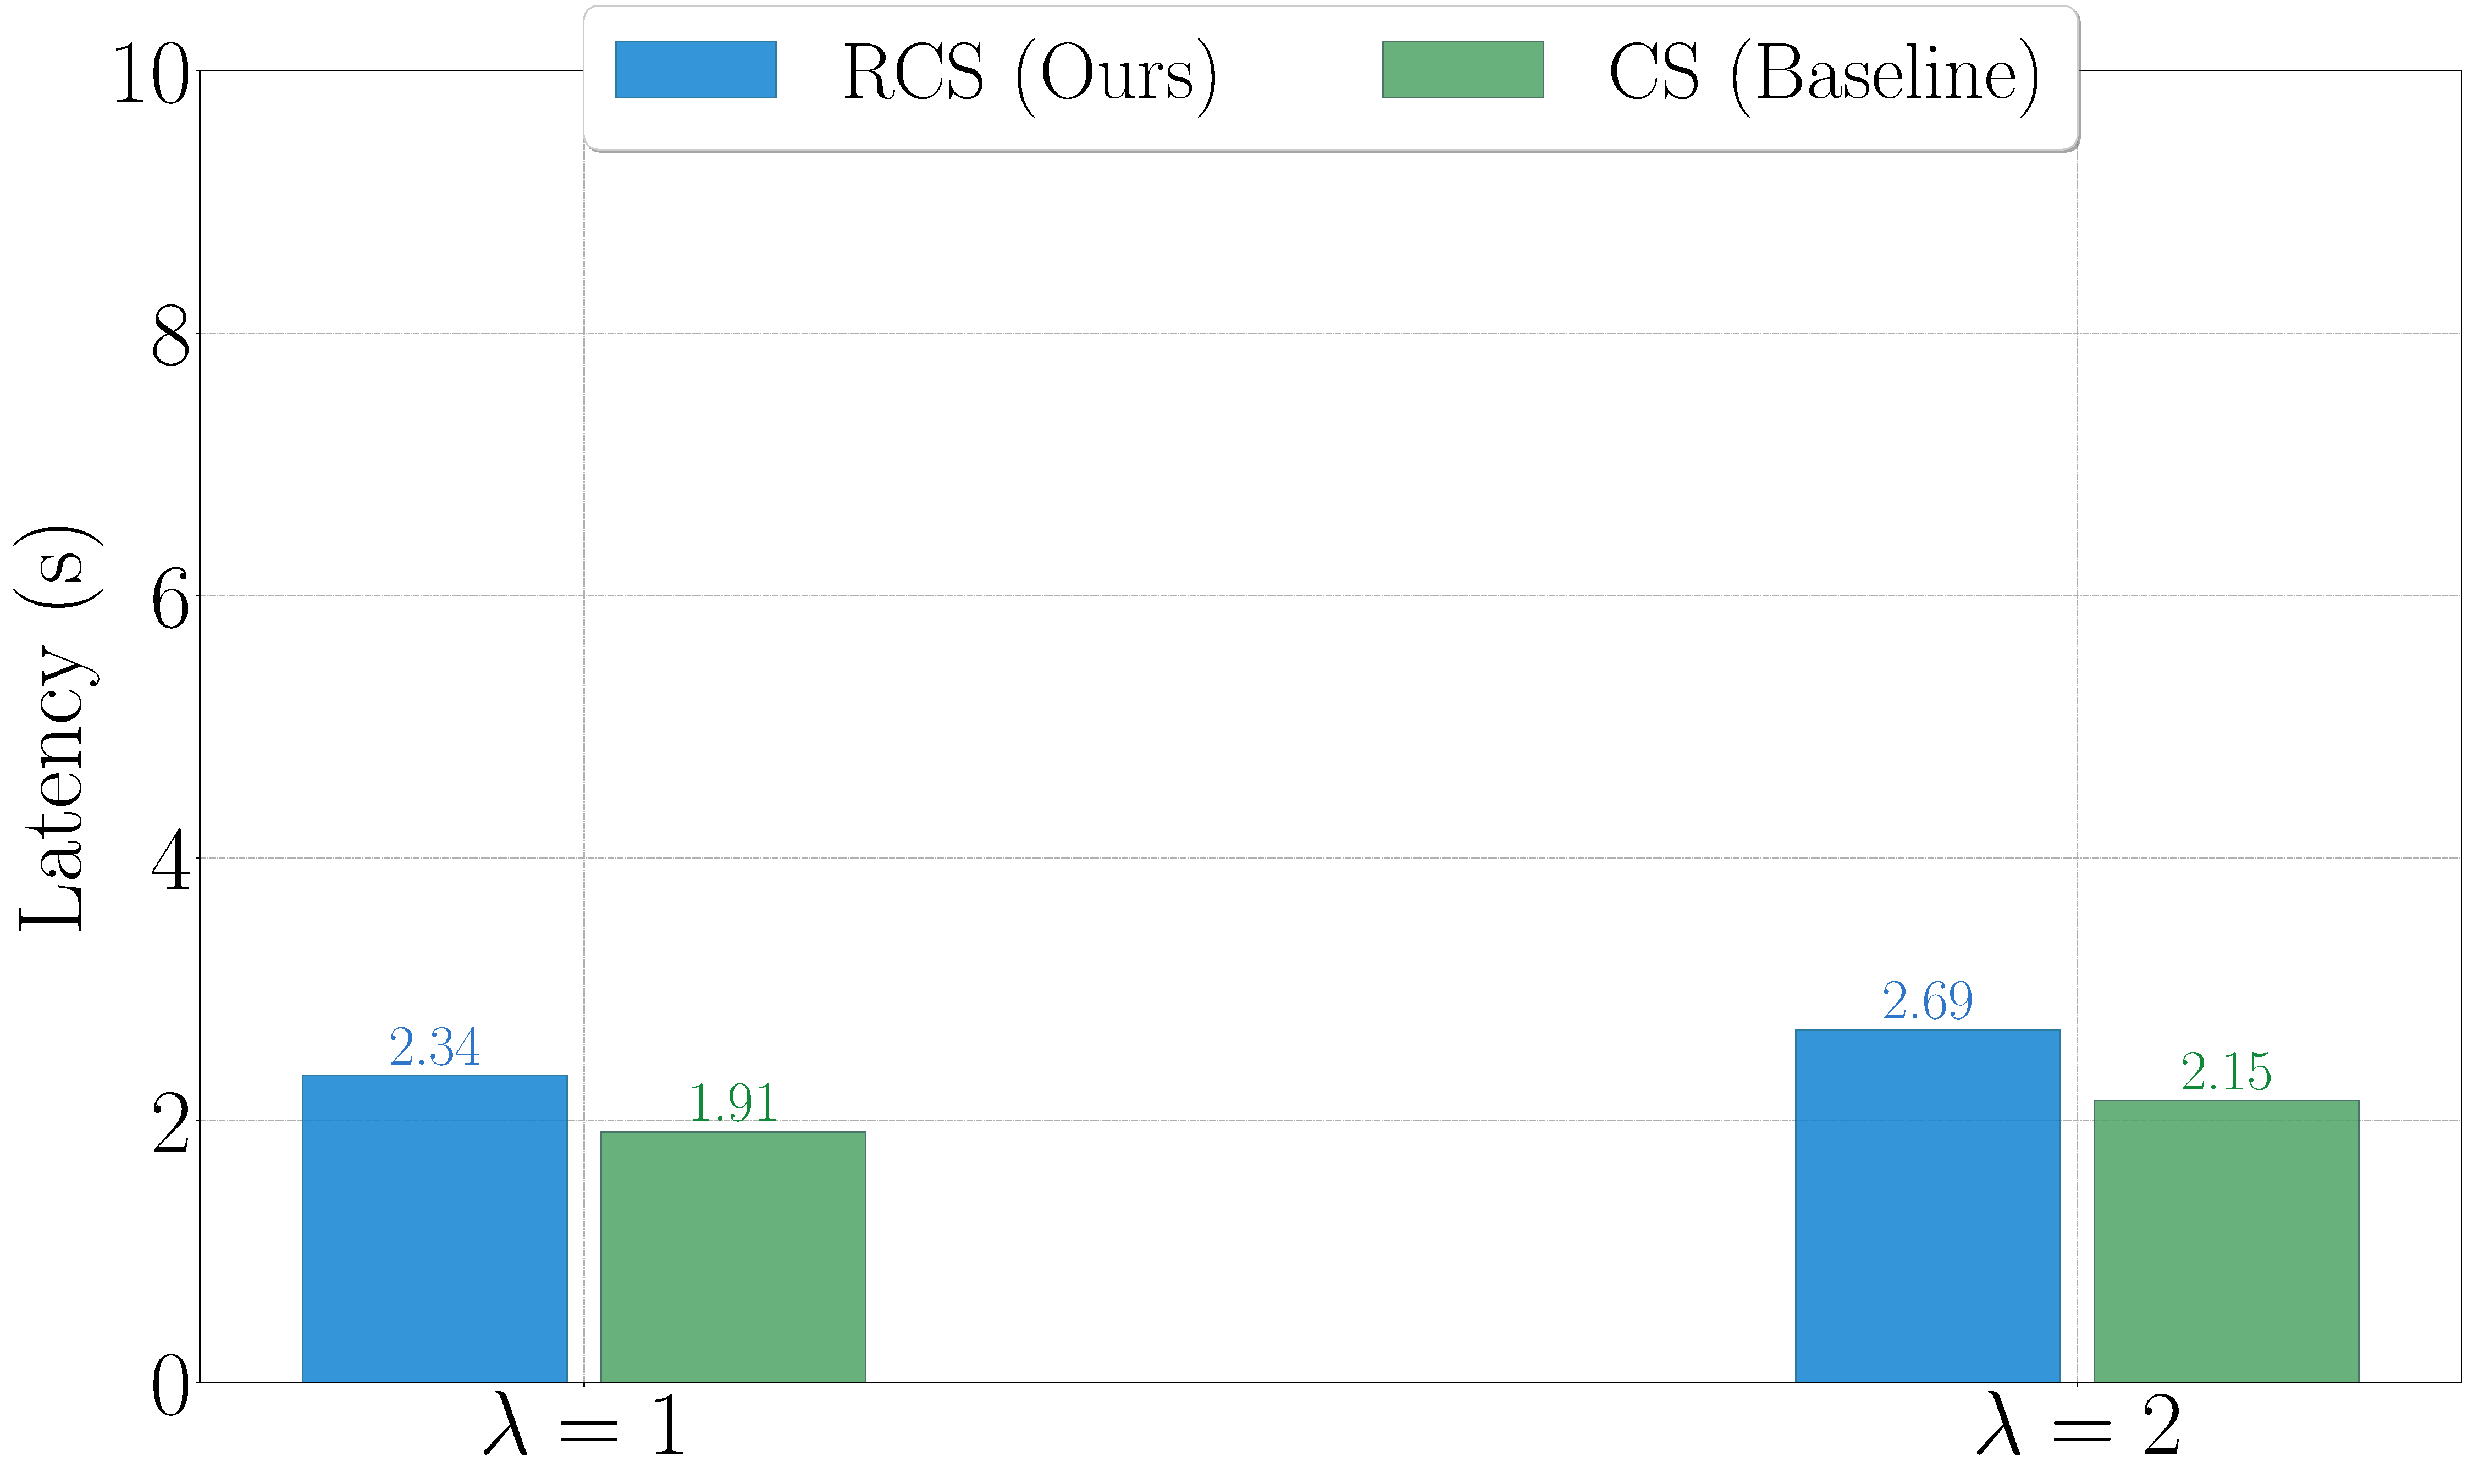
\includegraphics[width=\linewidth]{latex/eval_res/TC-5.pdf}
        \caption{$n=5$.}
    \end{subfigure}
    \begin{subfigure}{0.31\textwidth}
        \centering
        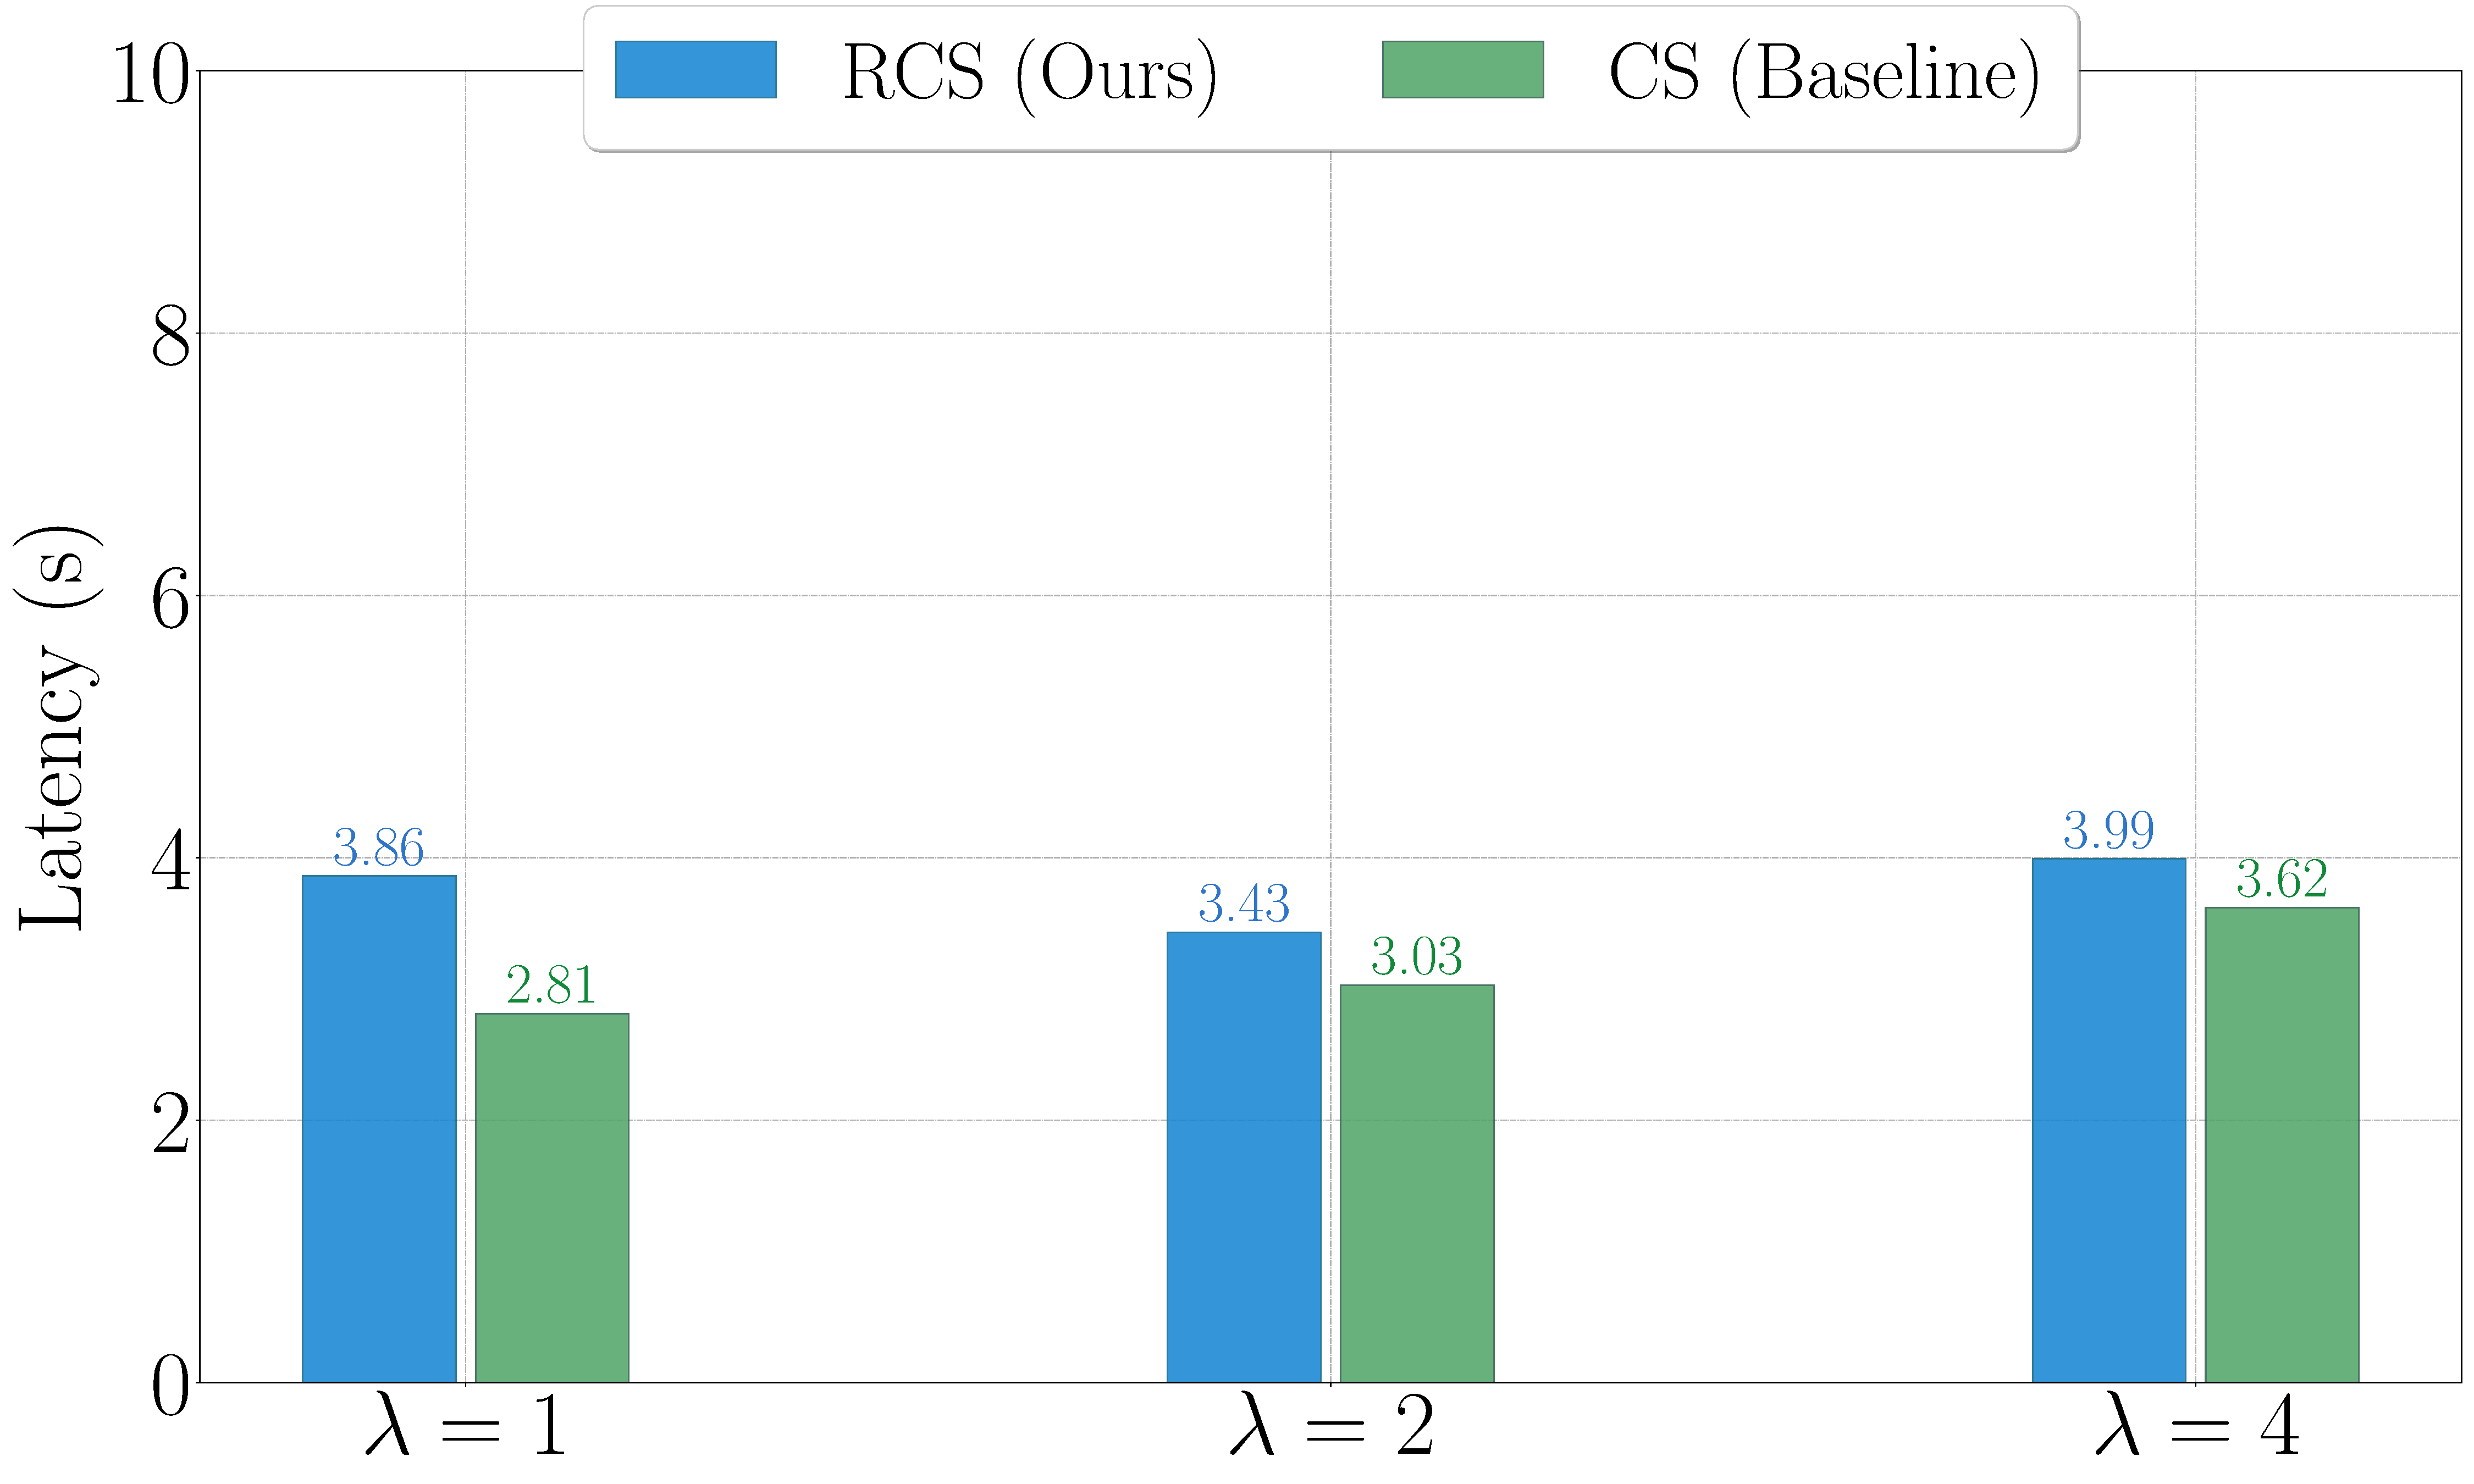
\includegraphics[width=\linewidth]{latex/eval_res/TC-9.pdf}
        \caption{$n=9$.}
    \end{subfigure}
    \begin{subfigure}{0.31\textwidth}
        \centering
        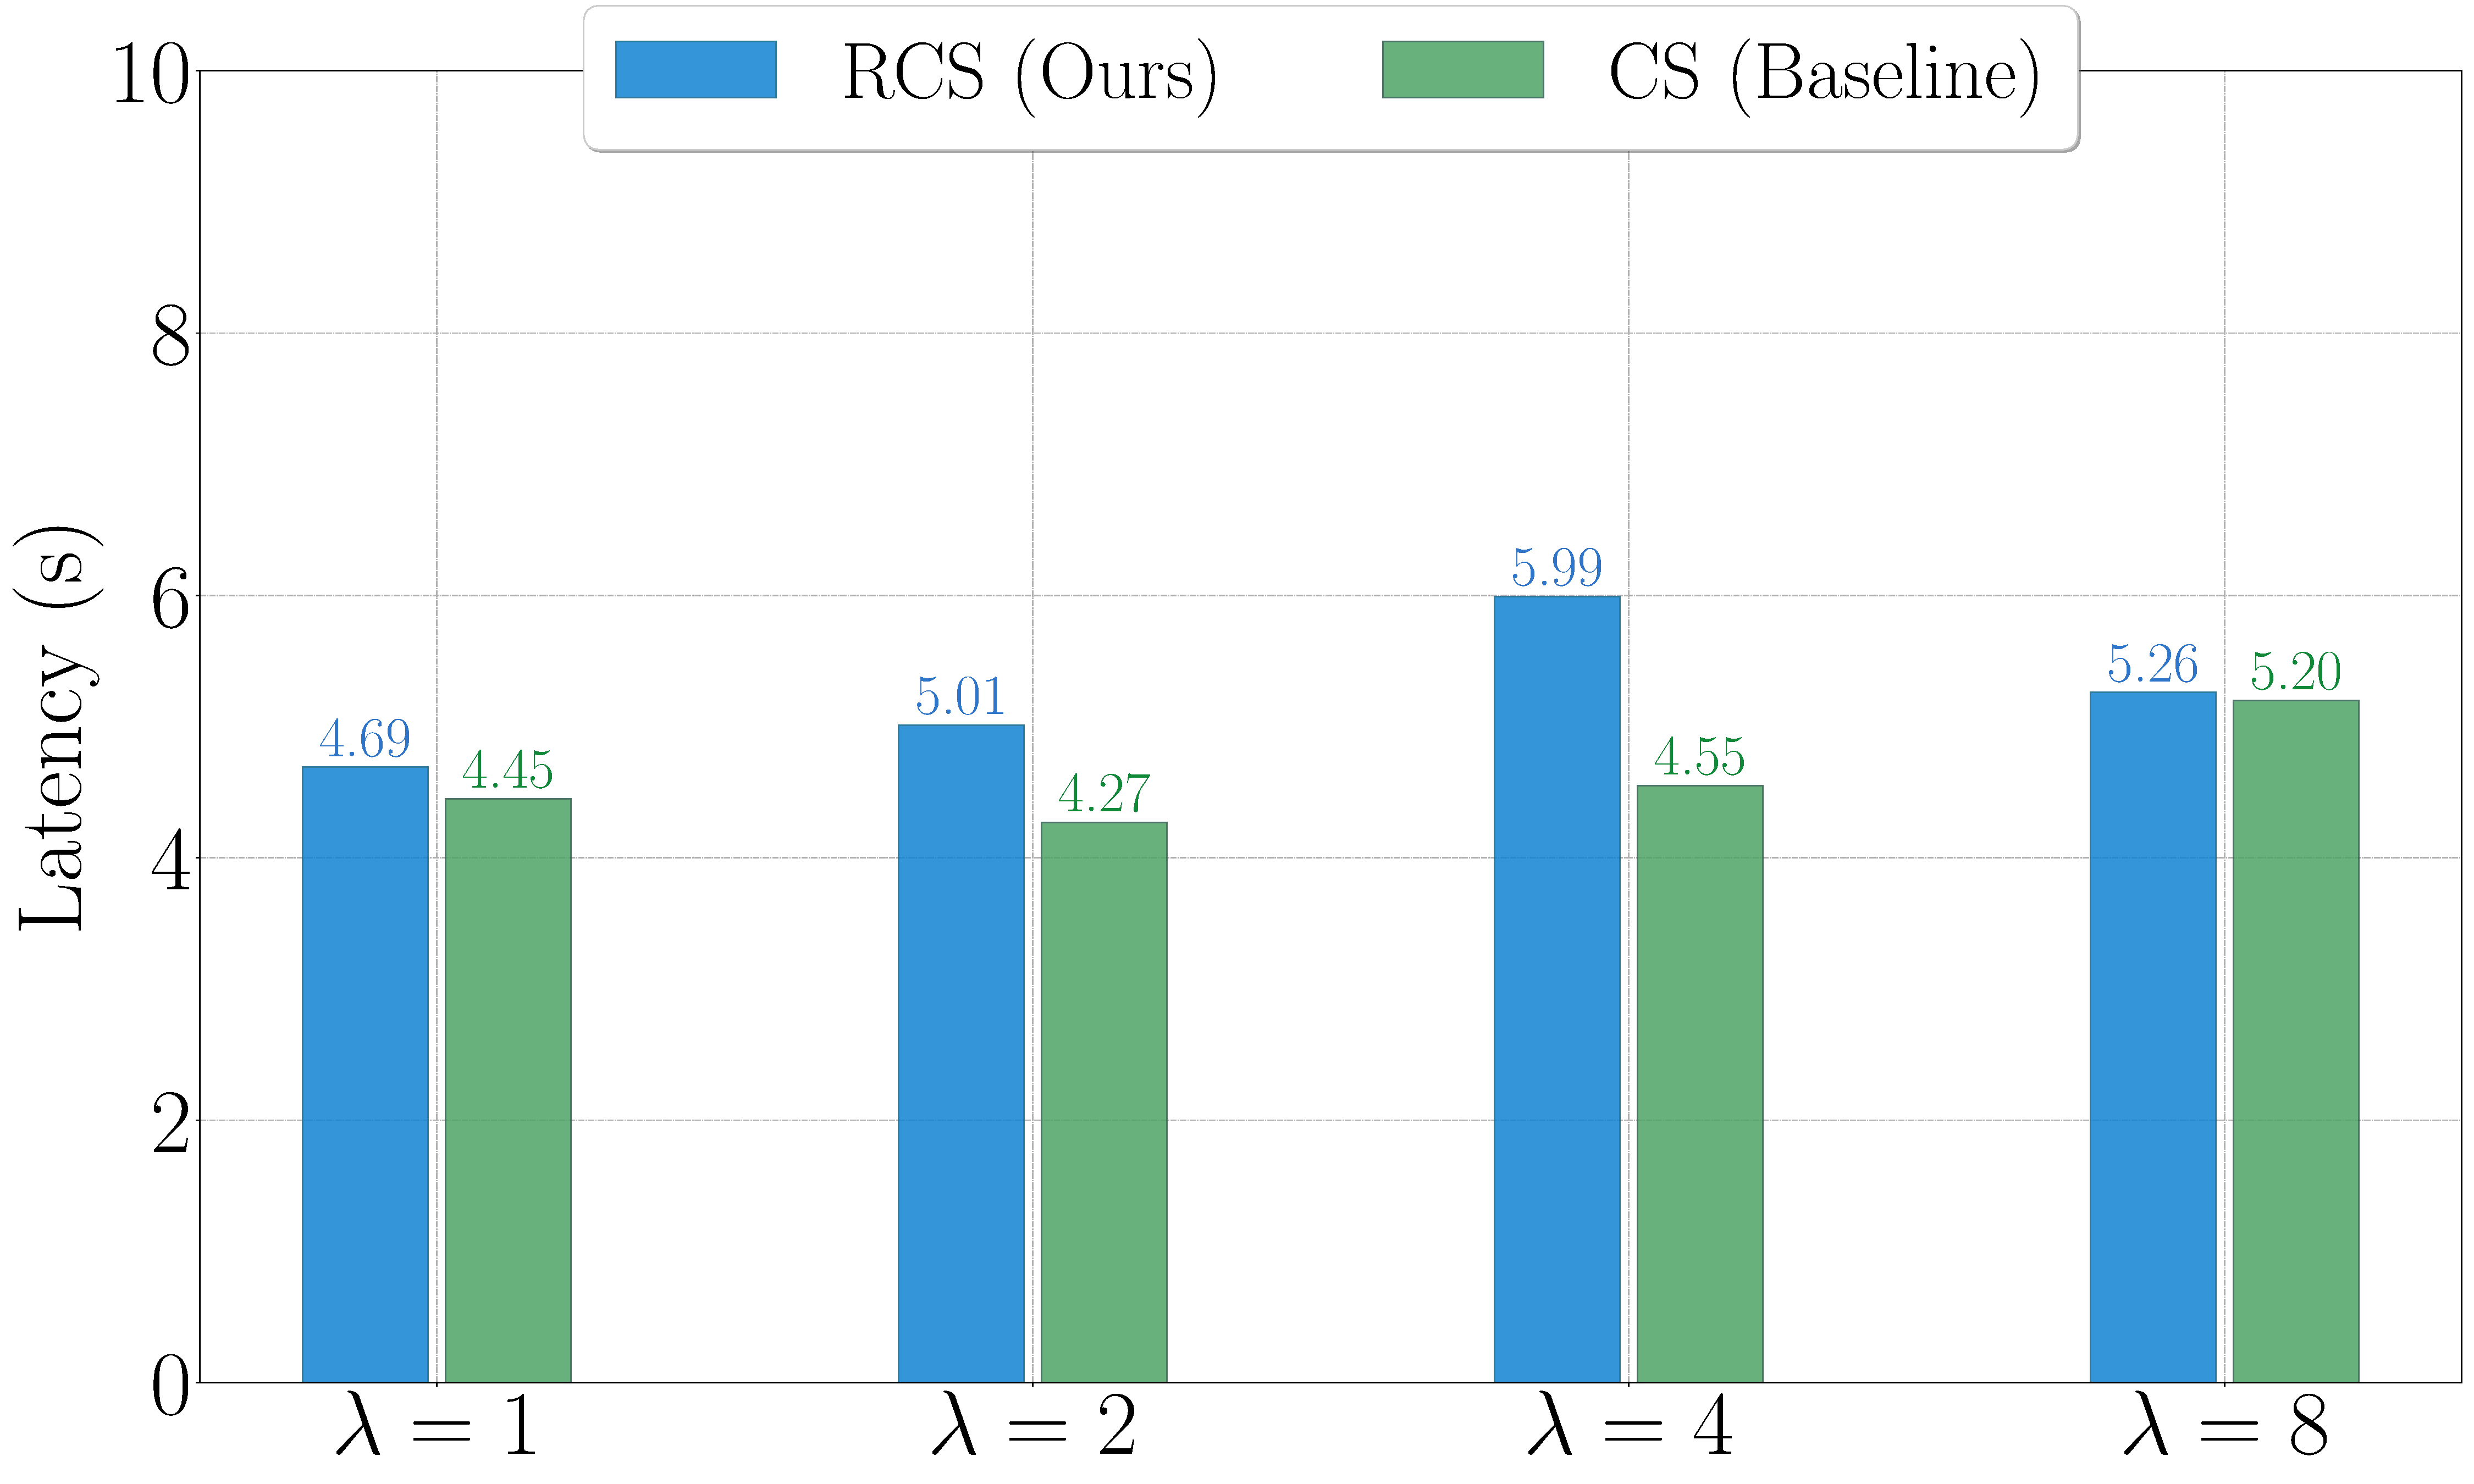
\includegraphics[width=\linewidth]{latex/eval_res/TC-17.pdf}
        \caption{$n=17$.}
    \end{subfigure}
    \caption{Evaluation results for the latency when $f < \lceil \frac{n}{2} \rceil$.}
    \label{fig:TC_g_app}
    % \vspace{-15pt}
\end{figure*}



\begin{figure*}[h]
    \centering
    \begin{subfigure}{0.31\textwidth}
        \centering
        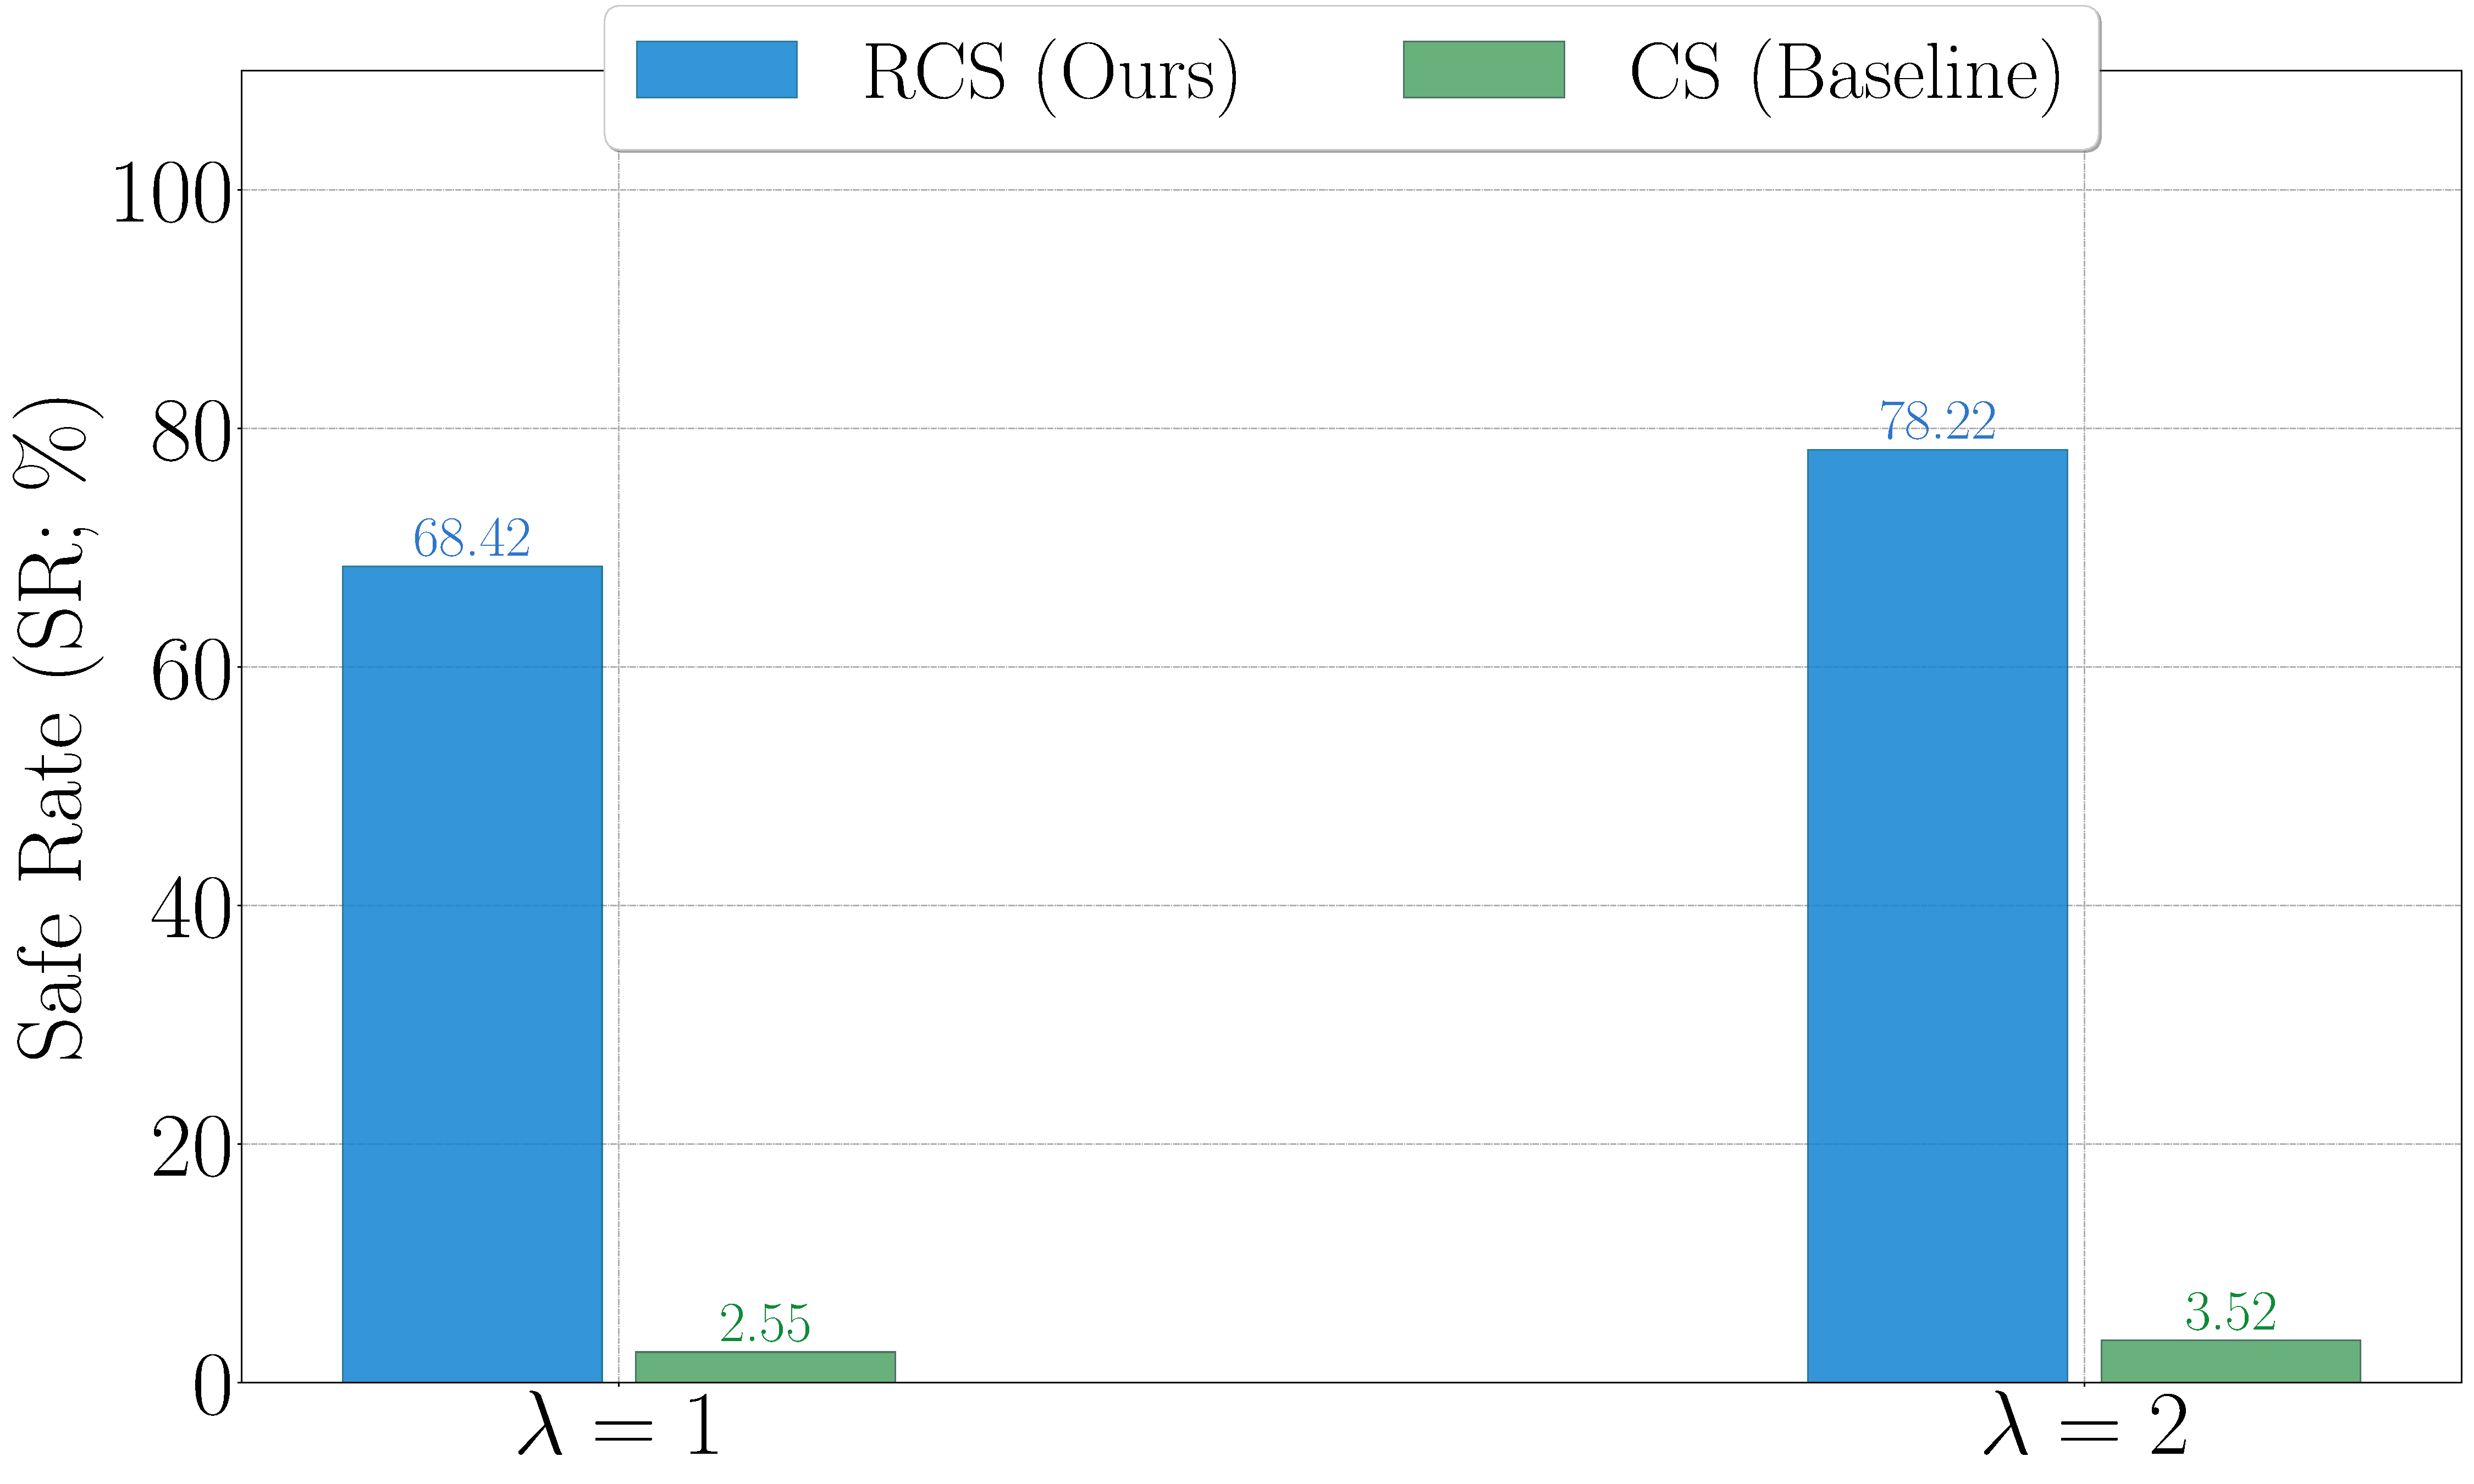
\includegraphics[width=\linewidth]{latex/eval_res_m/SR-5-m.pdf}
        \caption{$n=5$.}
    \end{subfigure}
    \begin{subfigure}{0.31\textwidth}
        \centering
        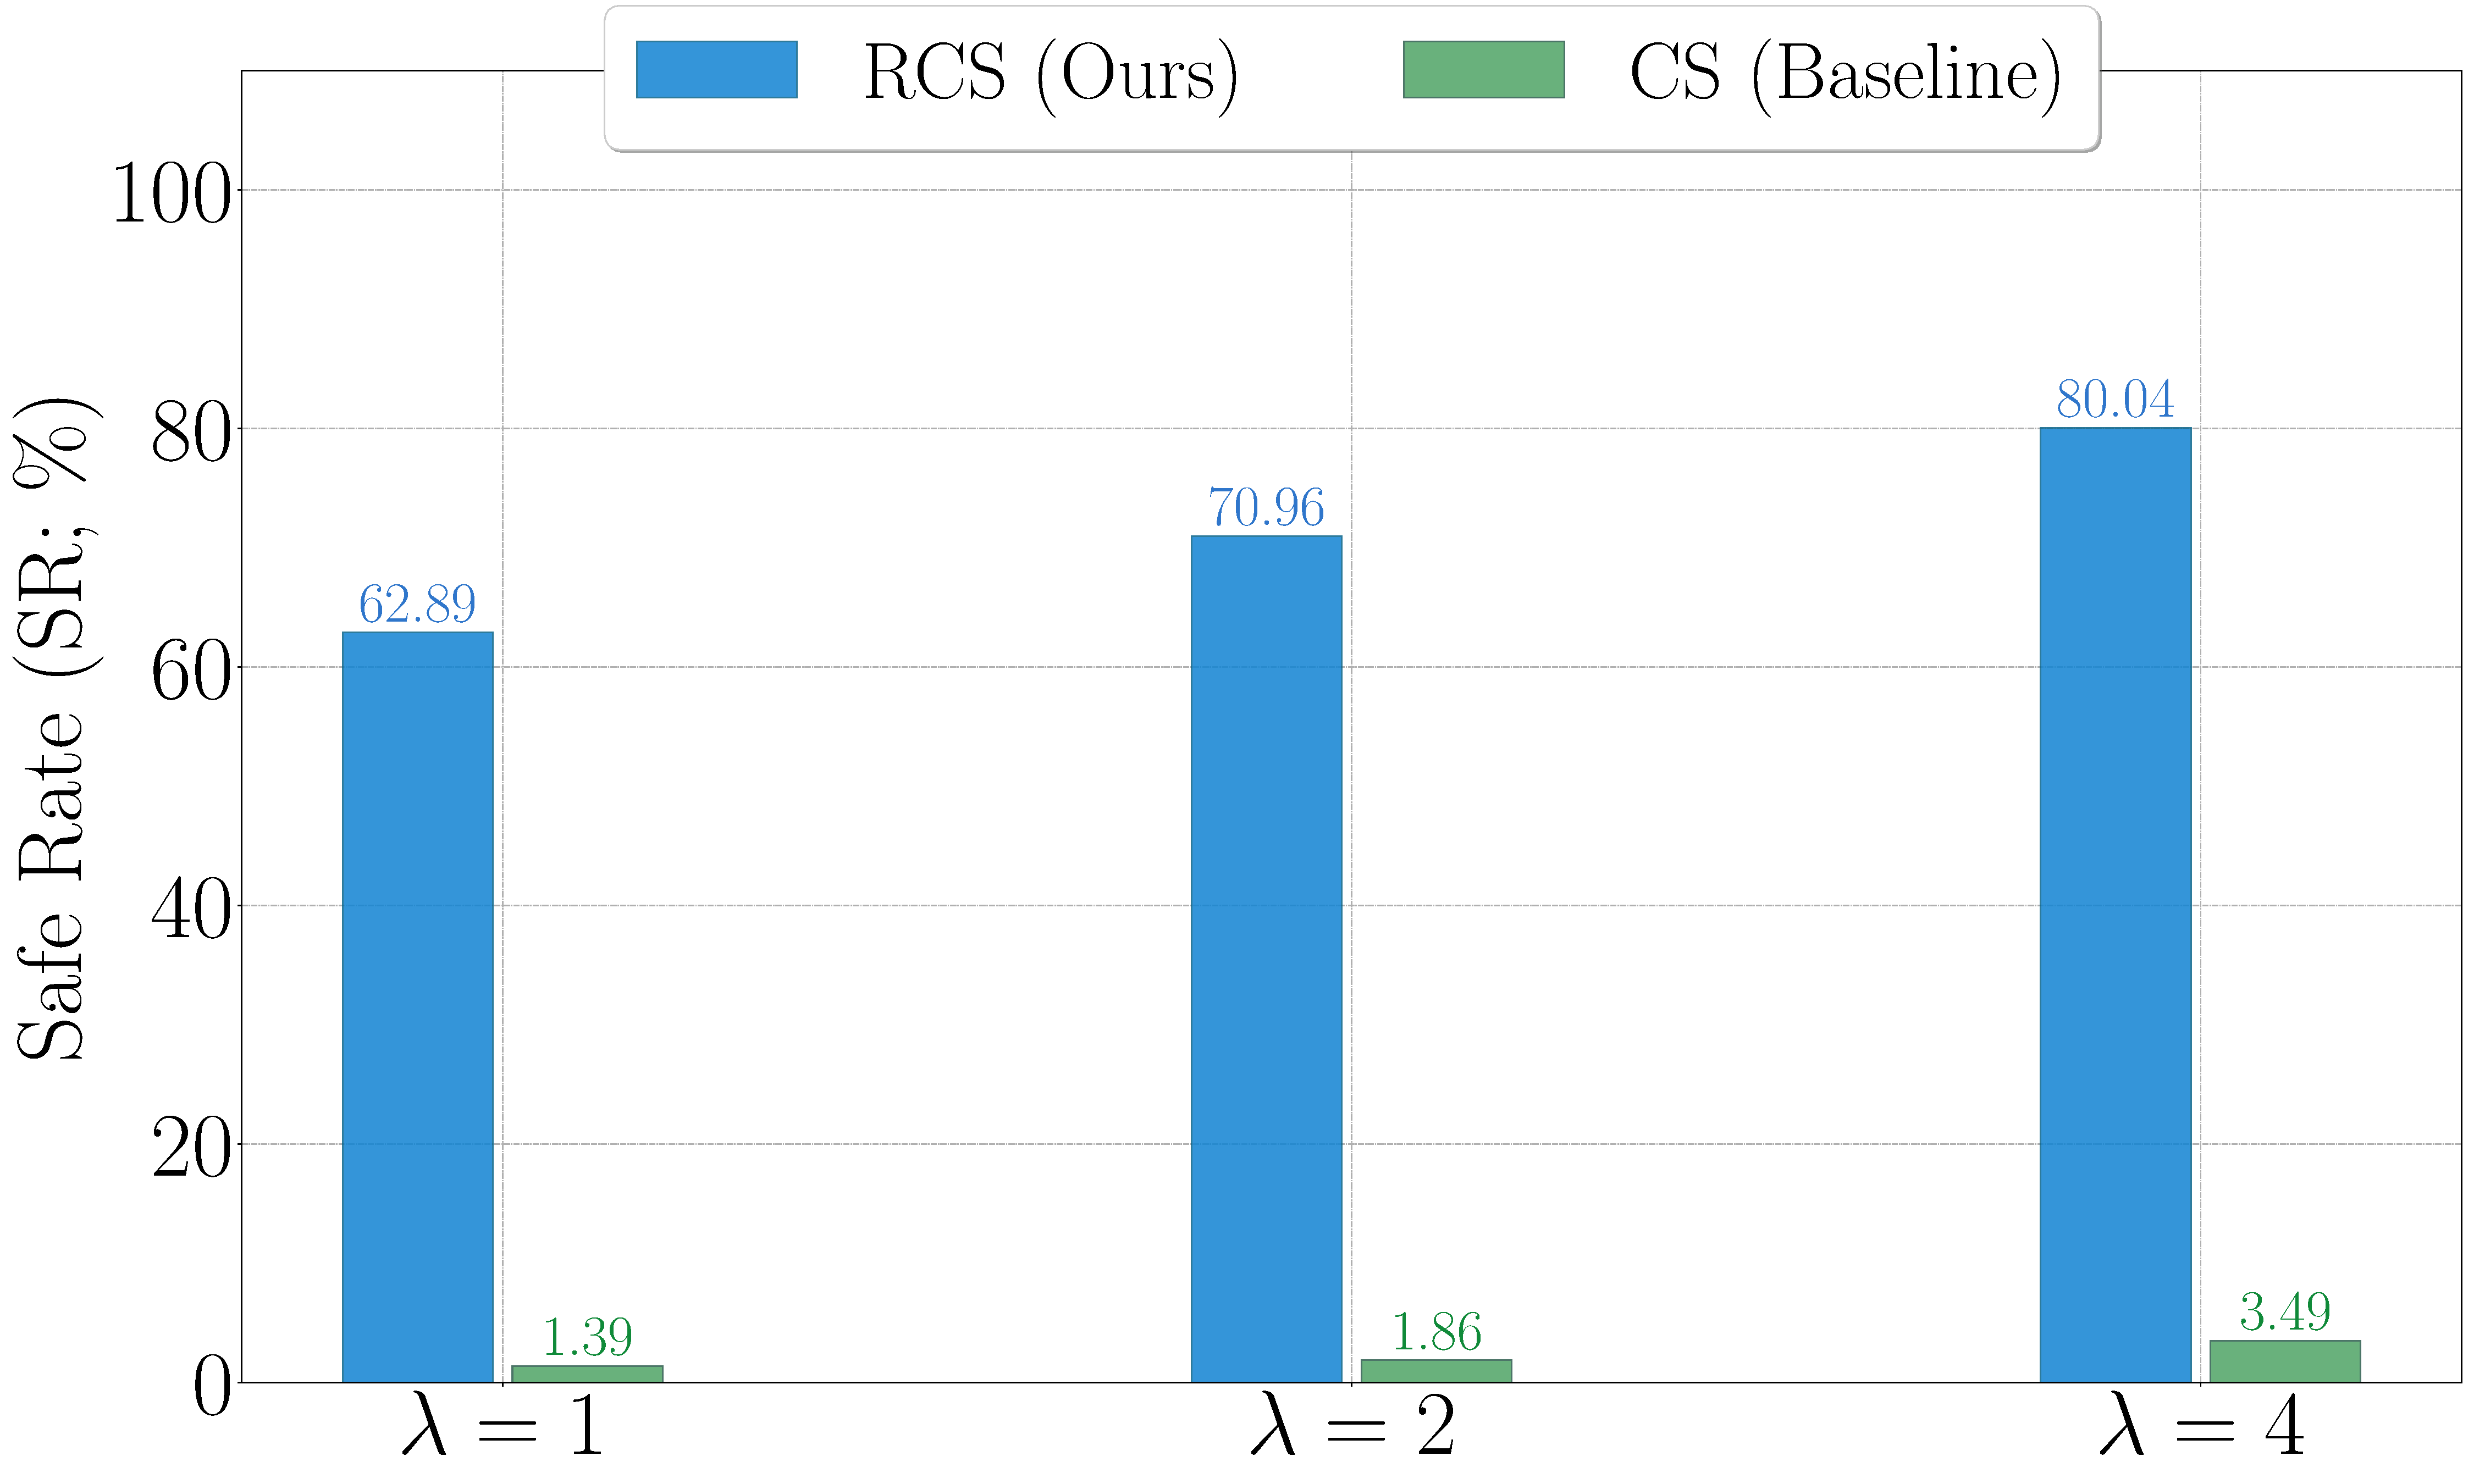
\includegraphics[width=\linewidth]{latex/eval_res_m/SR-9-m.pdf}
        \caption{$n=9$.}
    \end{subfigure}
    \begin{subfigure}{0.31\textwidth}
        \centering
        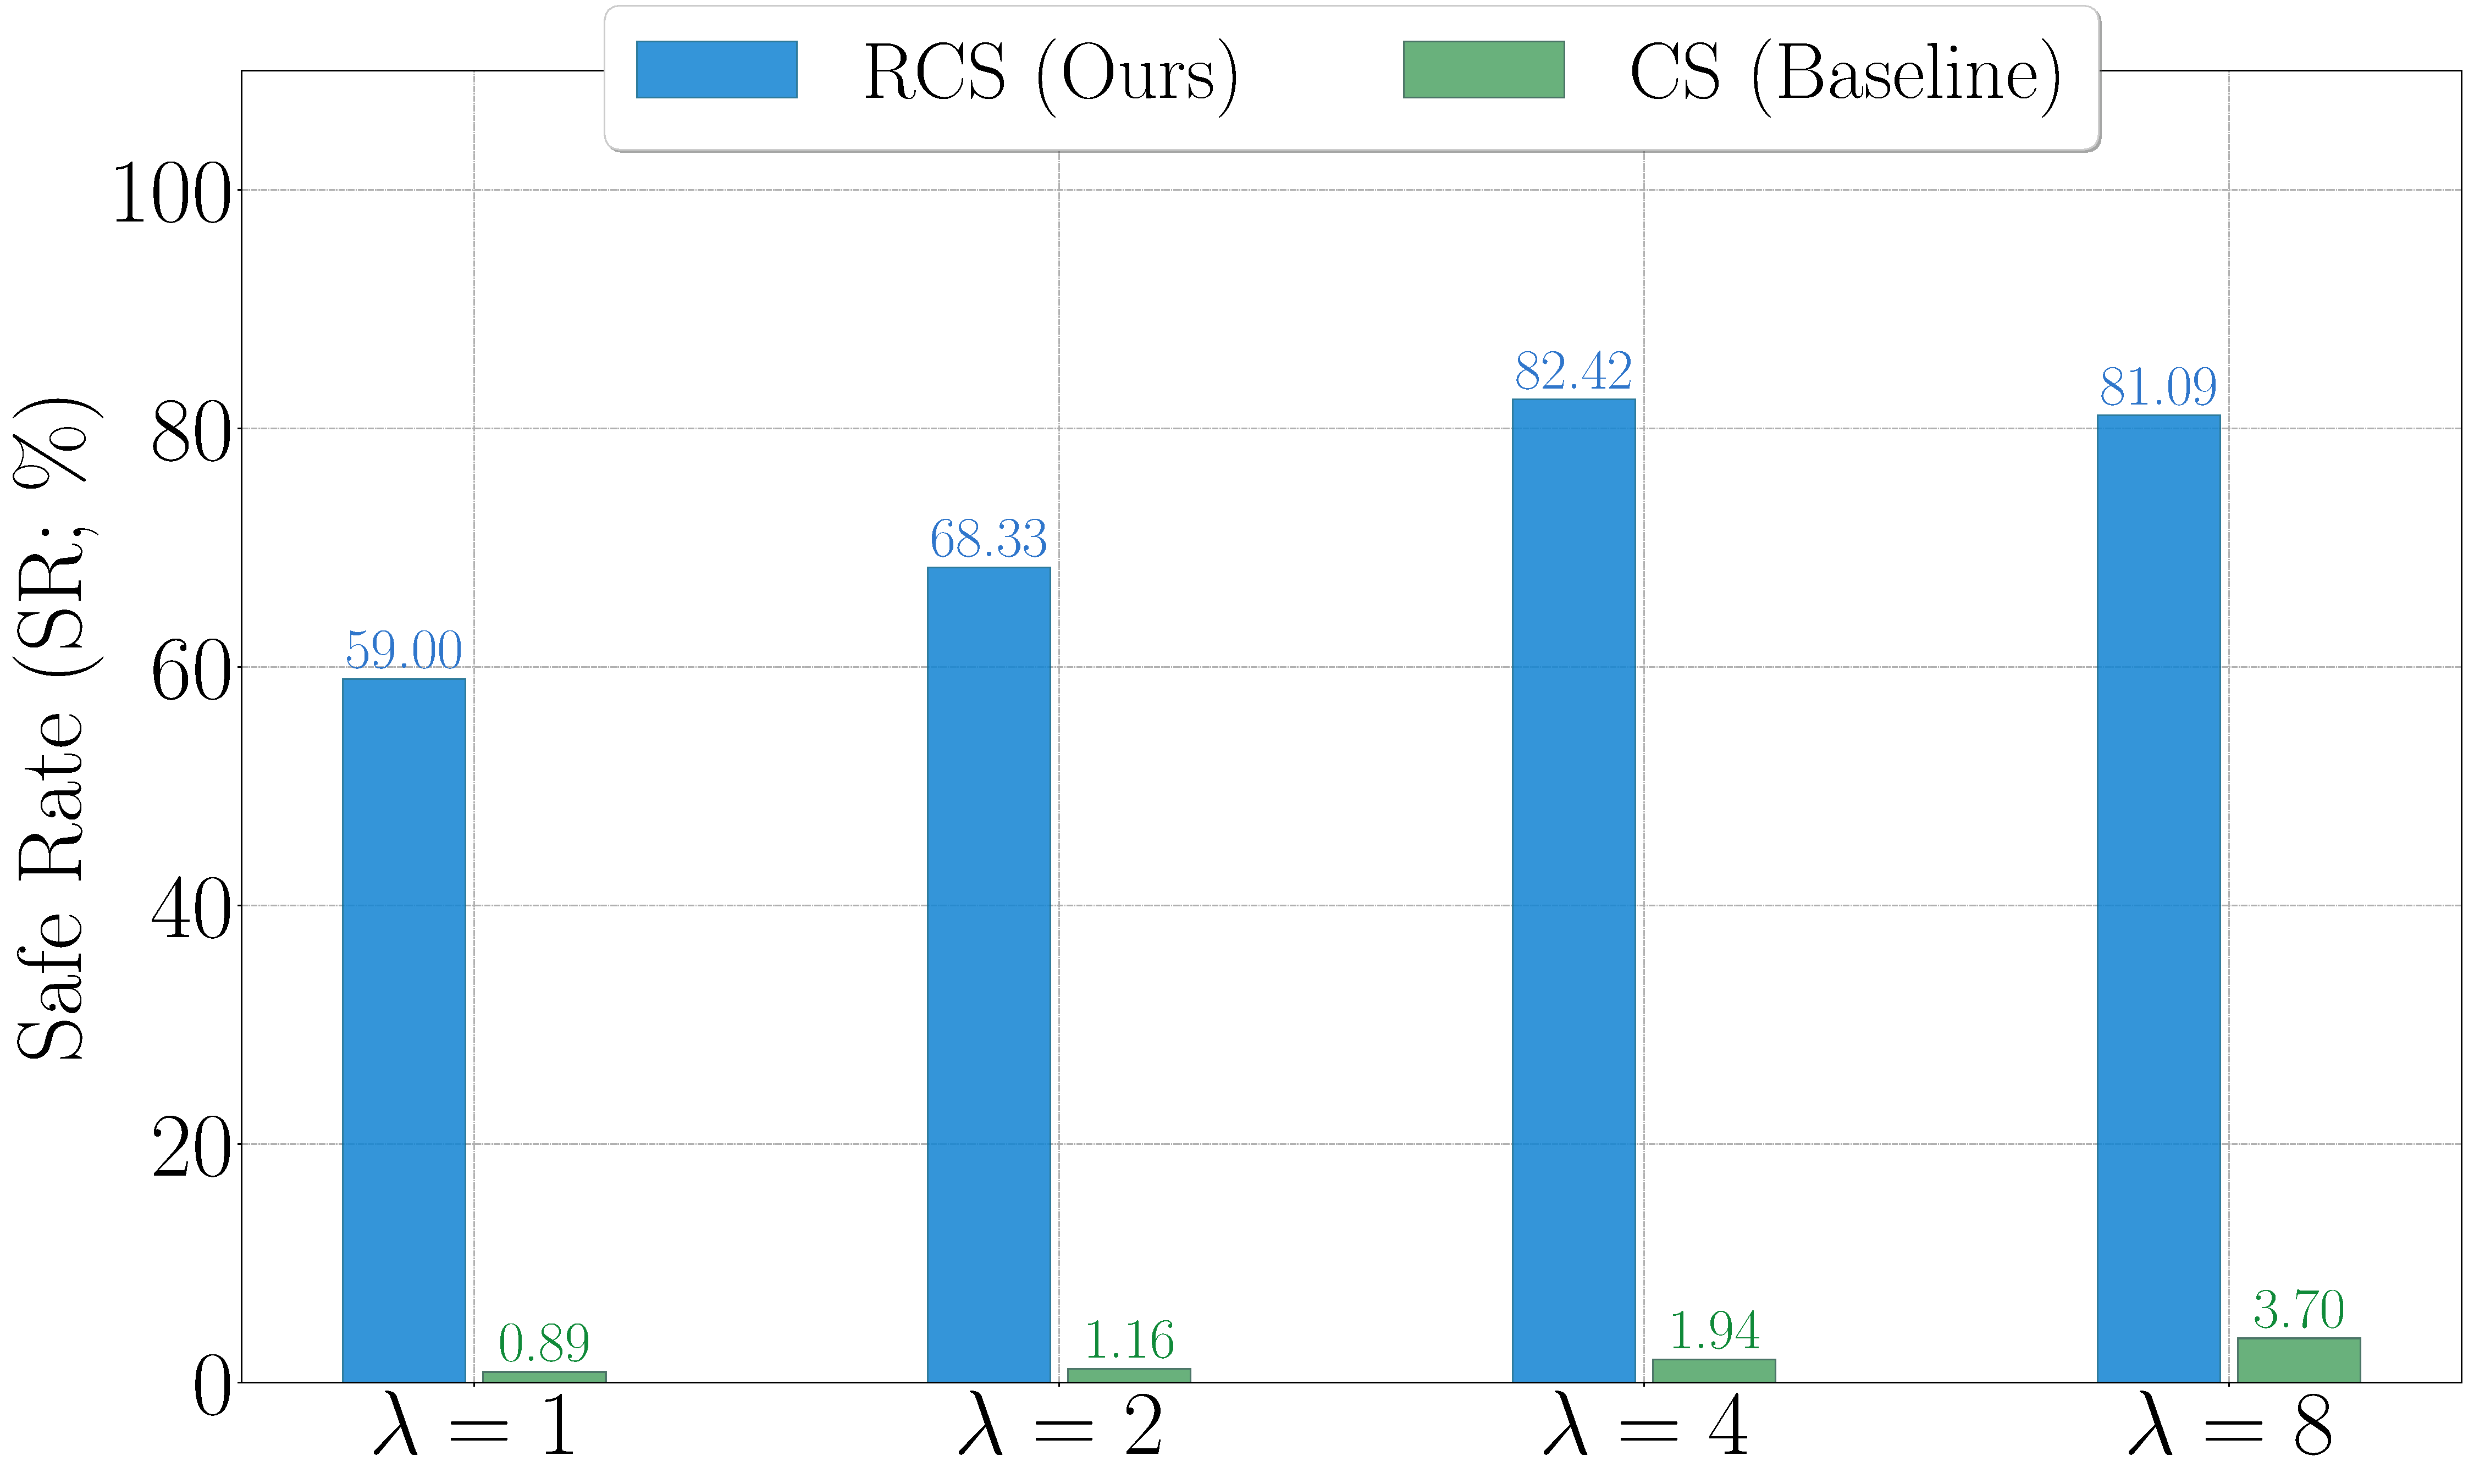
\includegraphics[width=\linewidth]{latex/eval_res_m/SR-17-m.pdf}
        \caption{$n=17$.}
    \end{subfigure}
    \caption{Evaluation results for the safe rate when Byzantine models collude.}
    \label{fig:sr_m_app}
    \vspace{-15pt}
\end{figure*}

\newpage
\begin{figure*}[!]
    \centering
    \begin{subfigure}{0.32\textwidth}
        \centering
        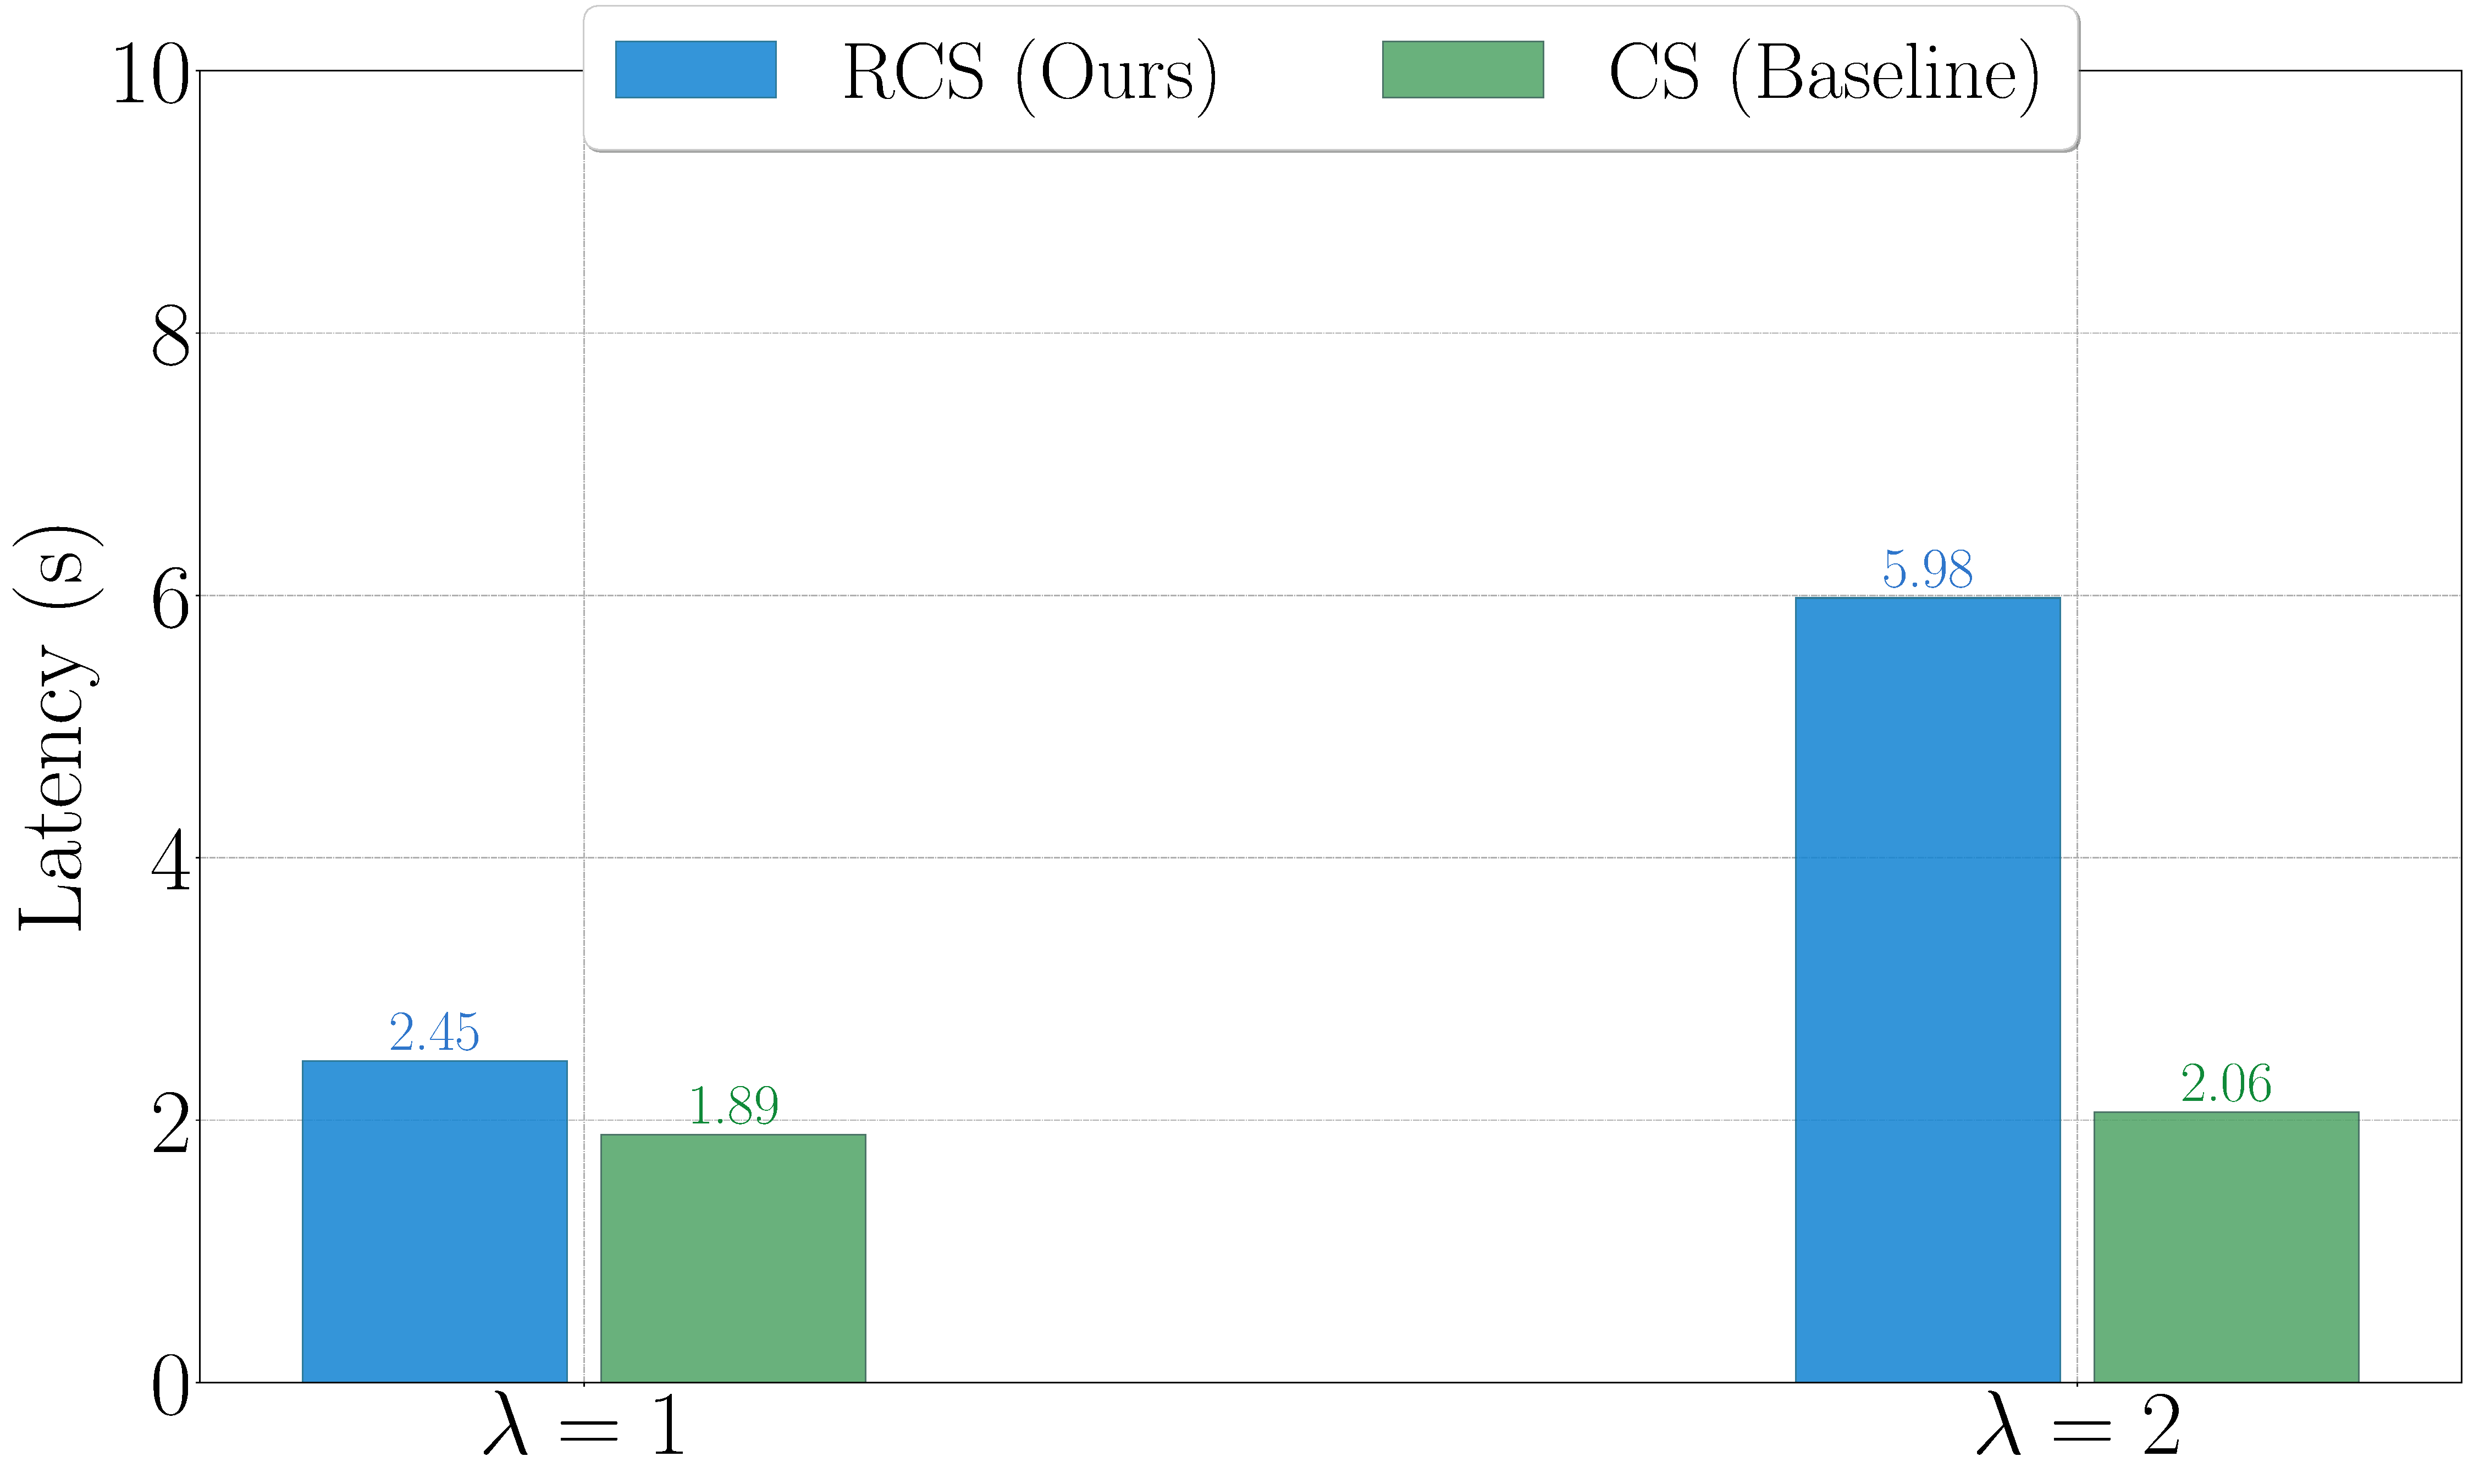
\includegraphics[width=\linewidth]{latex/eval_res_m/TC-5-m.pdf}
        \caption{$n=5$.}
    \end{subfigure}
    \begin{subfigure}{0.32\textwidth}
        \centering
        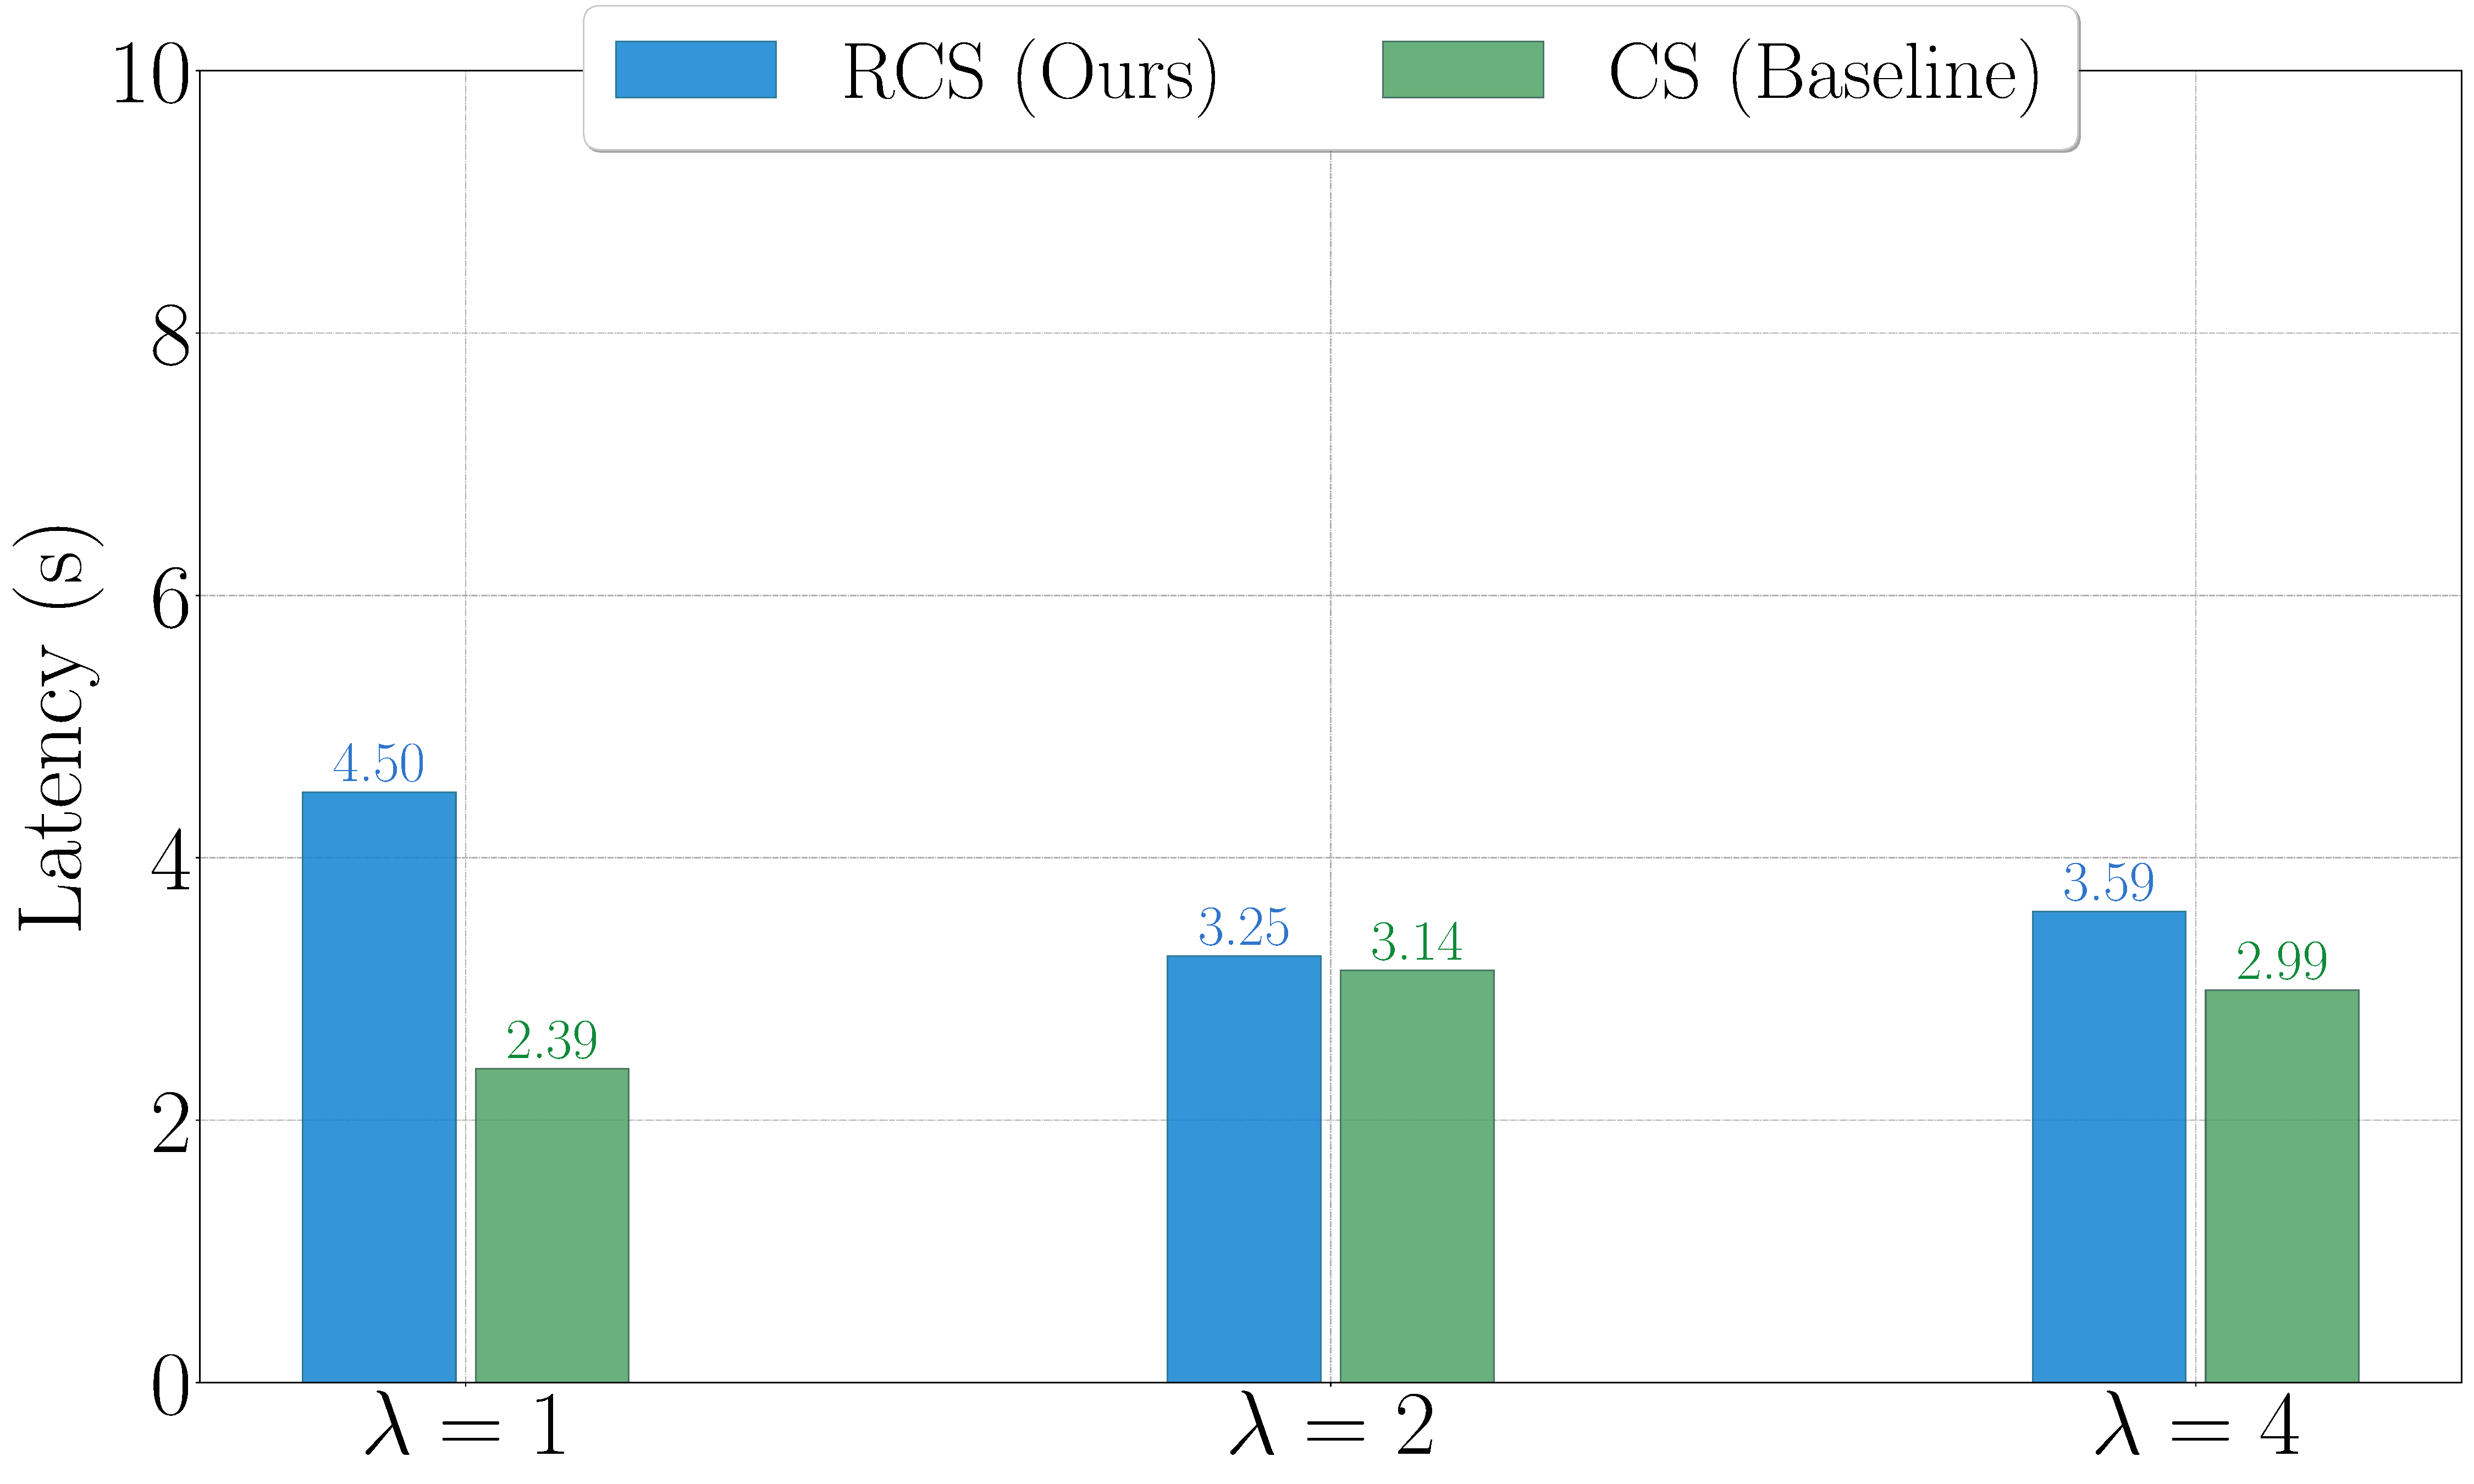
\includegraphics[width=\linewidth]{latex/eval_res_m/TC-9-m.pdf}
        \caption{$n=9$.}
    \end{subfigure}
    \begin{subfigure}{0.32\textwidth}
        \centering
        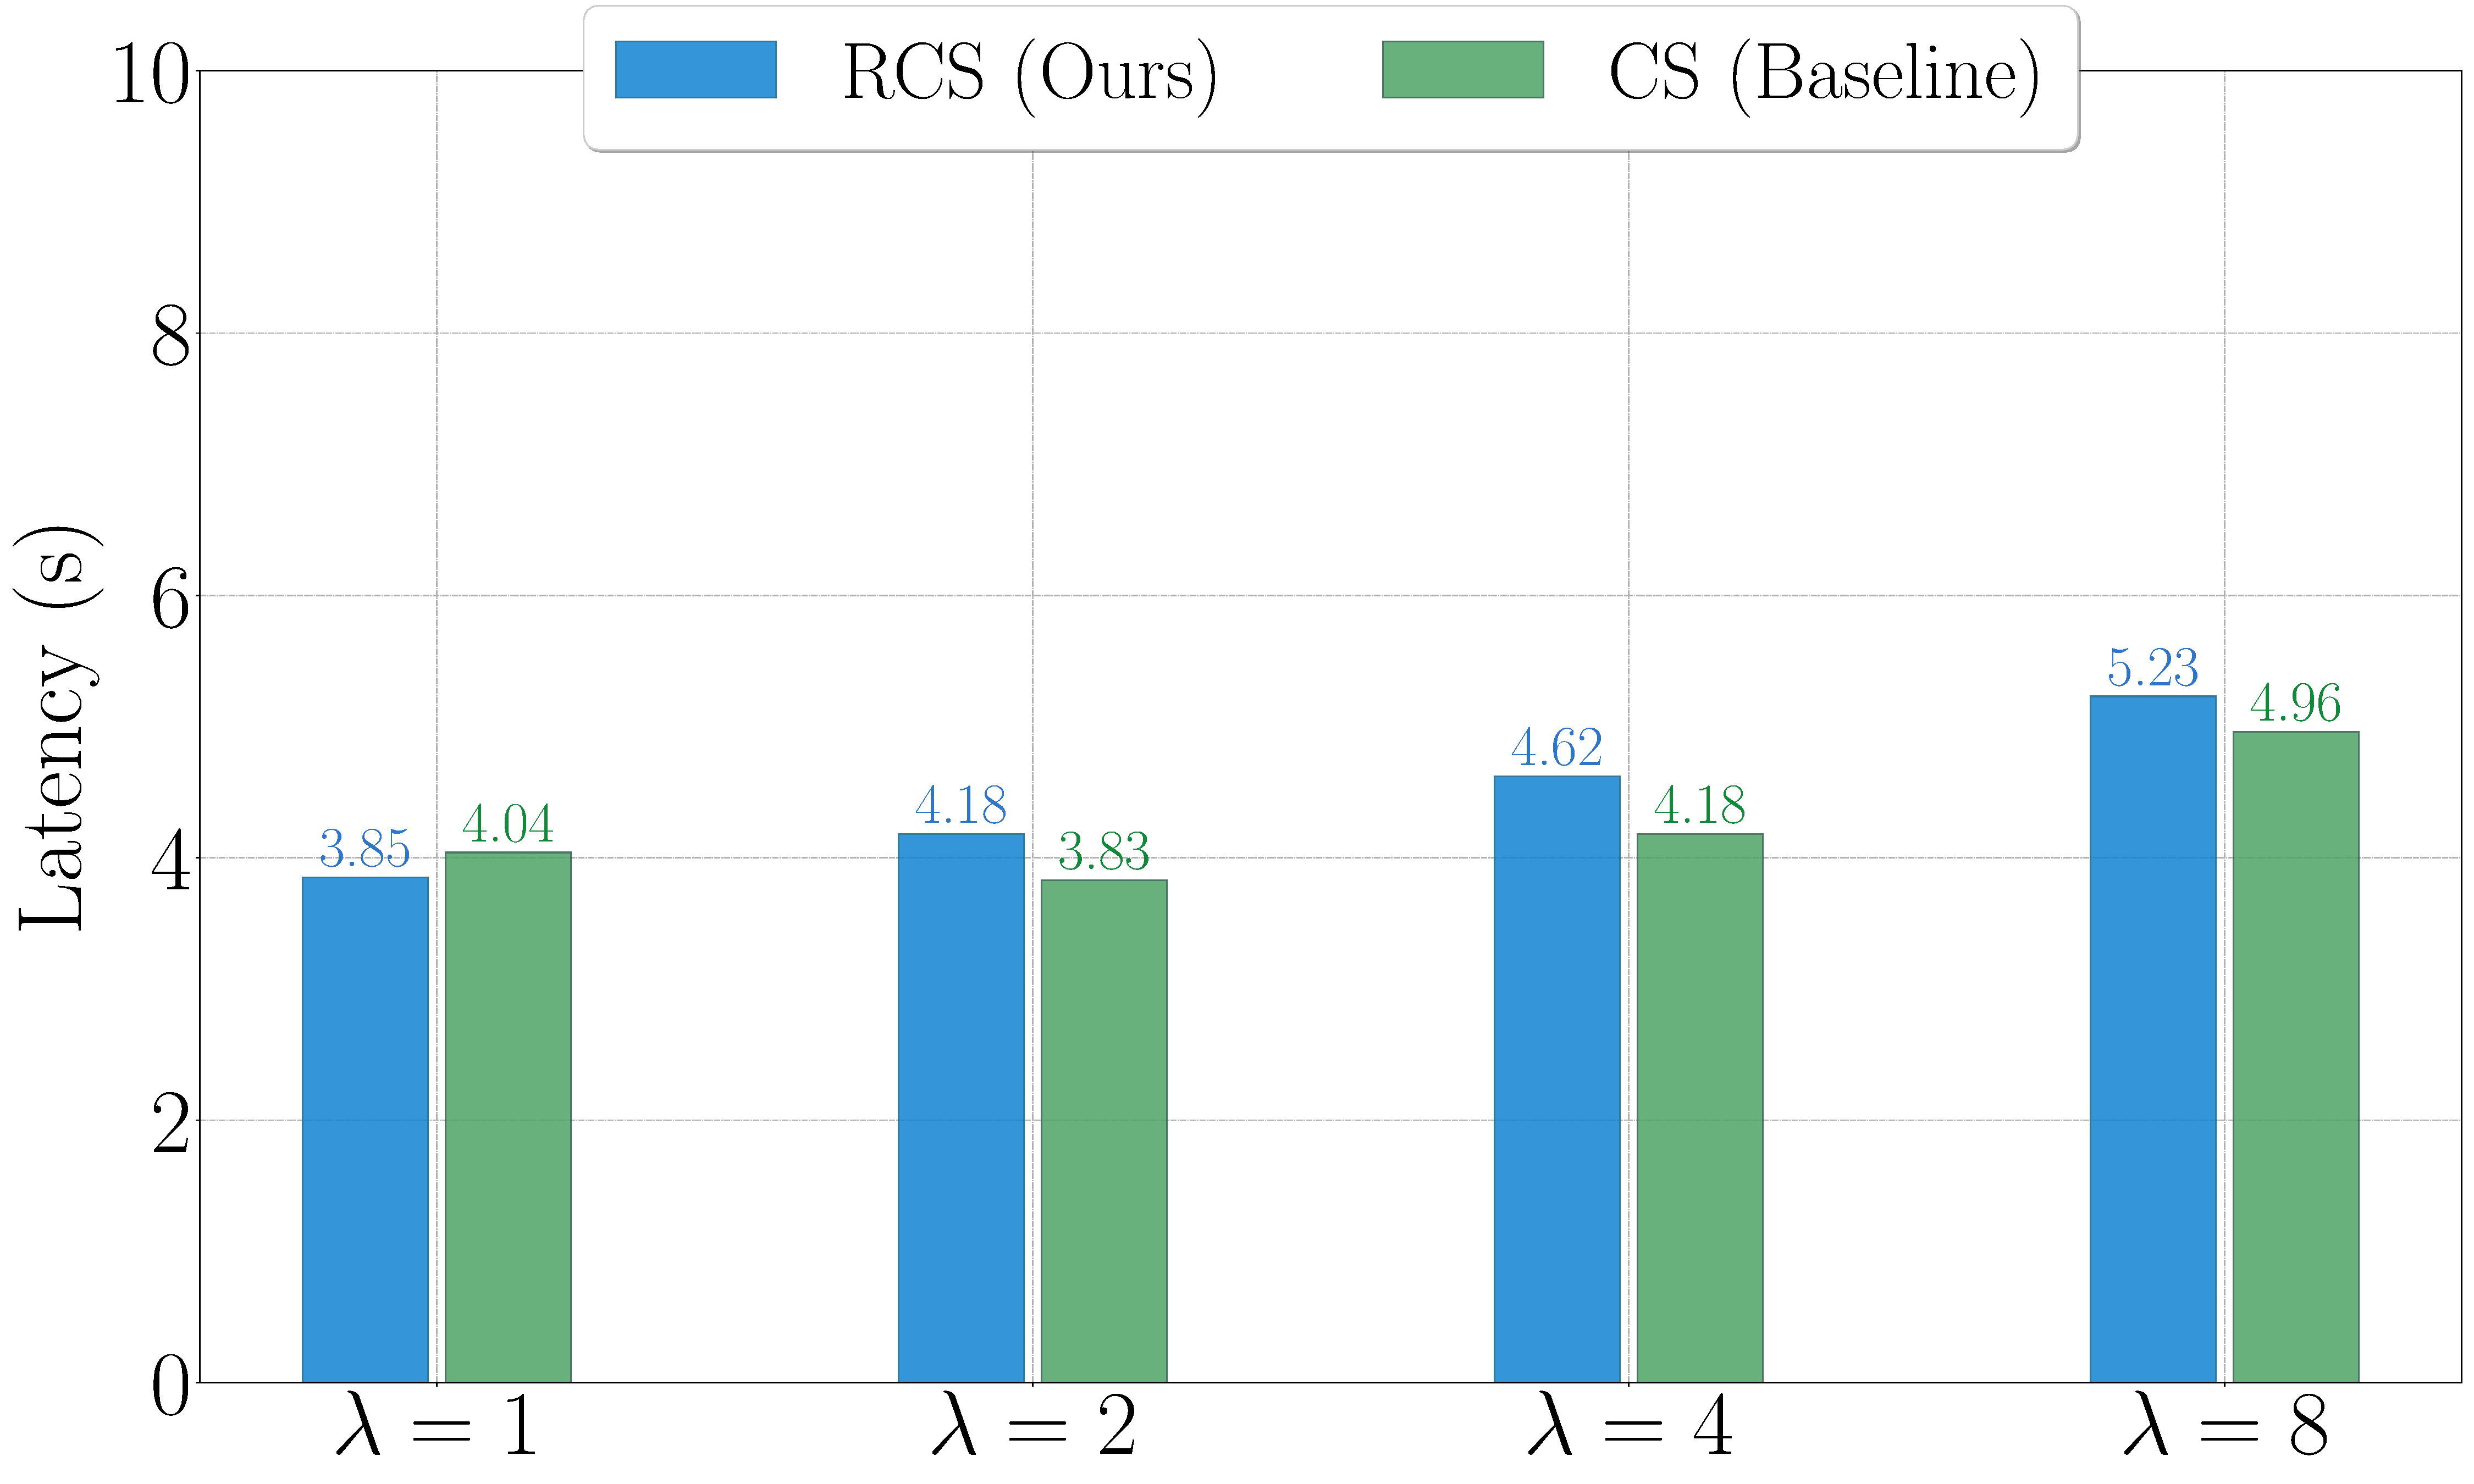
\includegraphics[width=\linewidth]{latex/eval_res_m/TC-17-m.pdf}
        \caption{$n=17$.}
    \end{subfigure}
    \caption{Evaluation results for the latency when Byzantine models collude.}
    \label{fig:TC_m_app}
    % \vspace{-15pt}
\end{figure*}

\begin{figure*}[!]
    \centering
    \begin{subfigure}{0.31\textwidth}
        \centering
        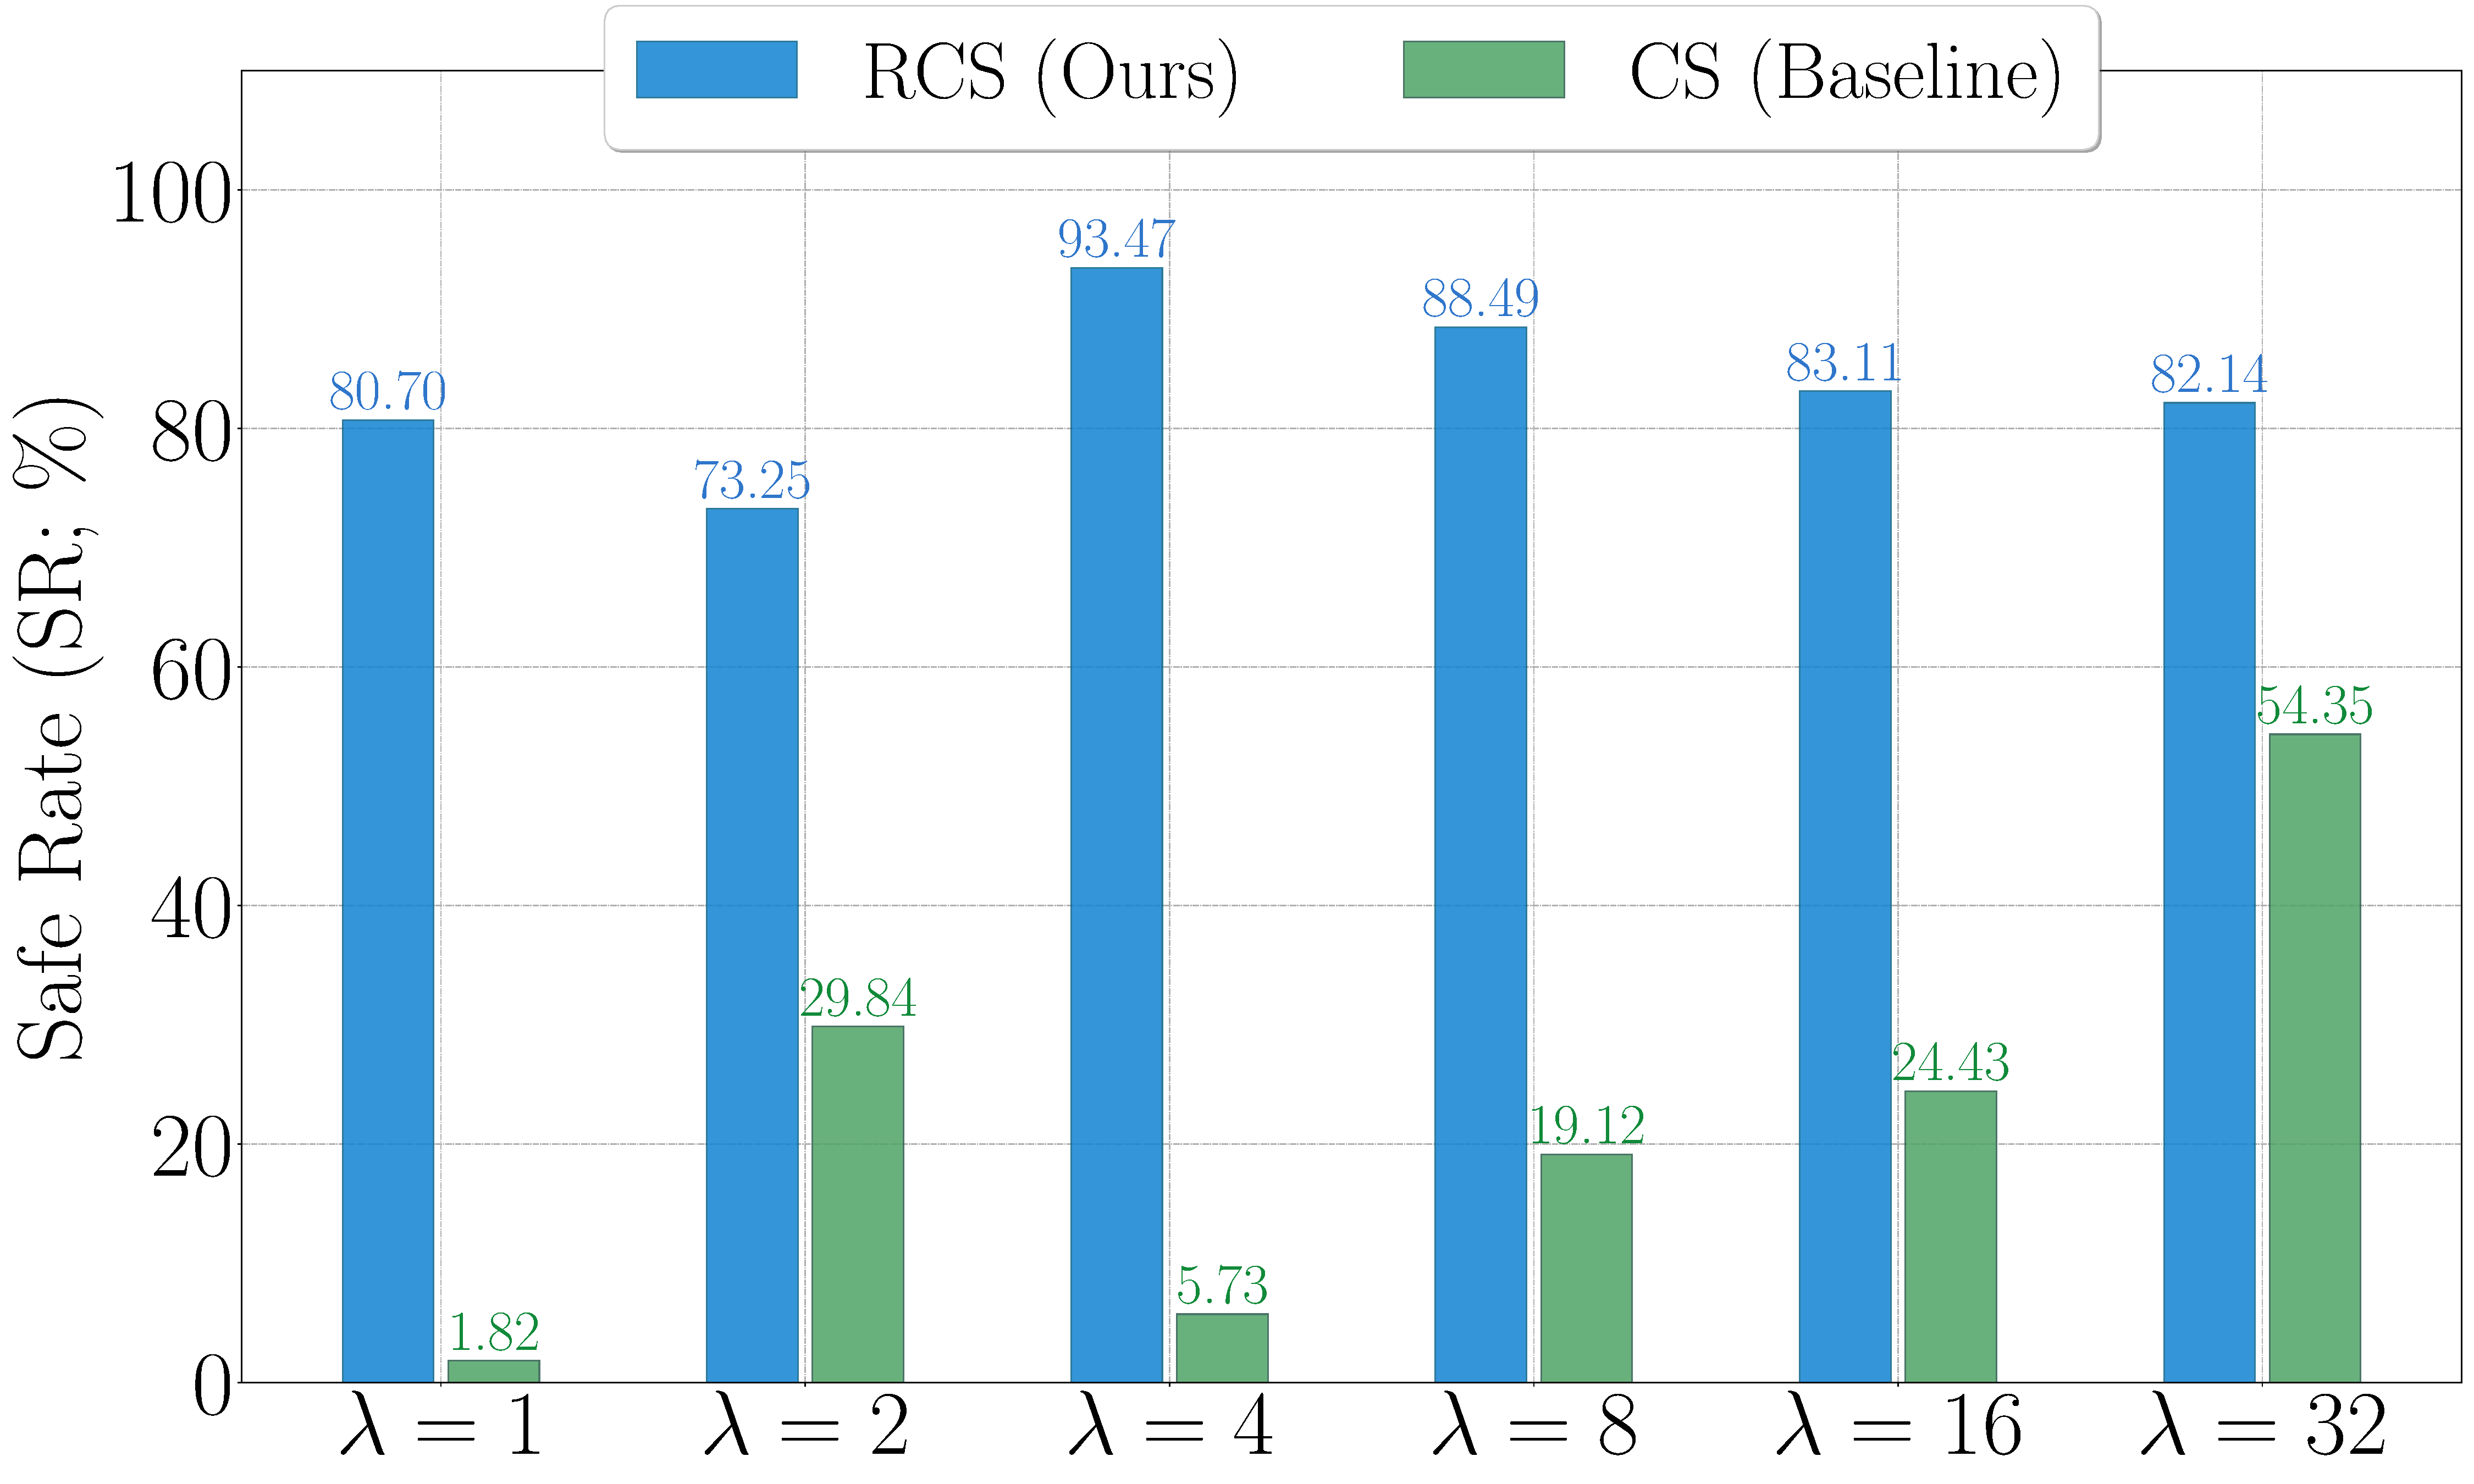
\includegraphics[width=\linewidth]{latex/eval_res_d/SR-34.pdf}
        \caption{$n=34$.}
    \end{subfigure}
    \begin{subfigure}{0.31\textwidth}
        \centering
        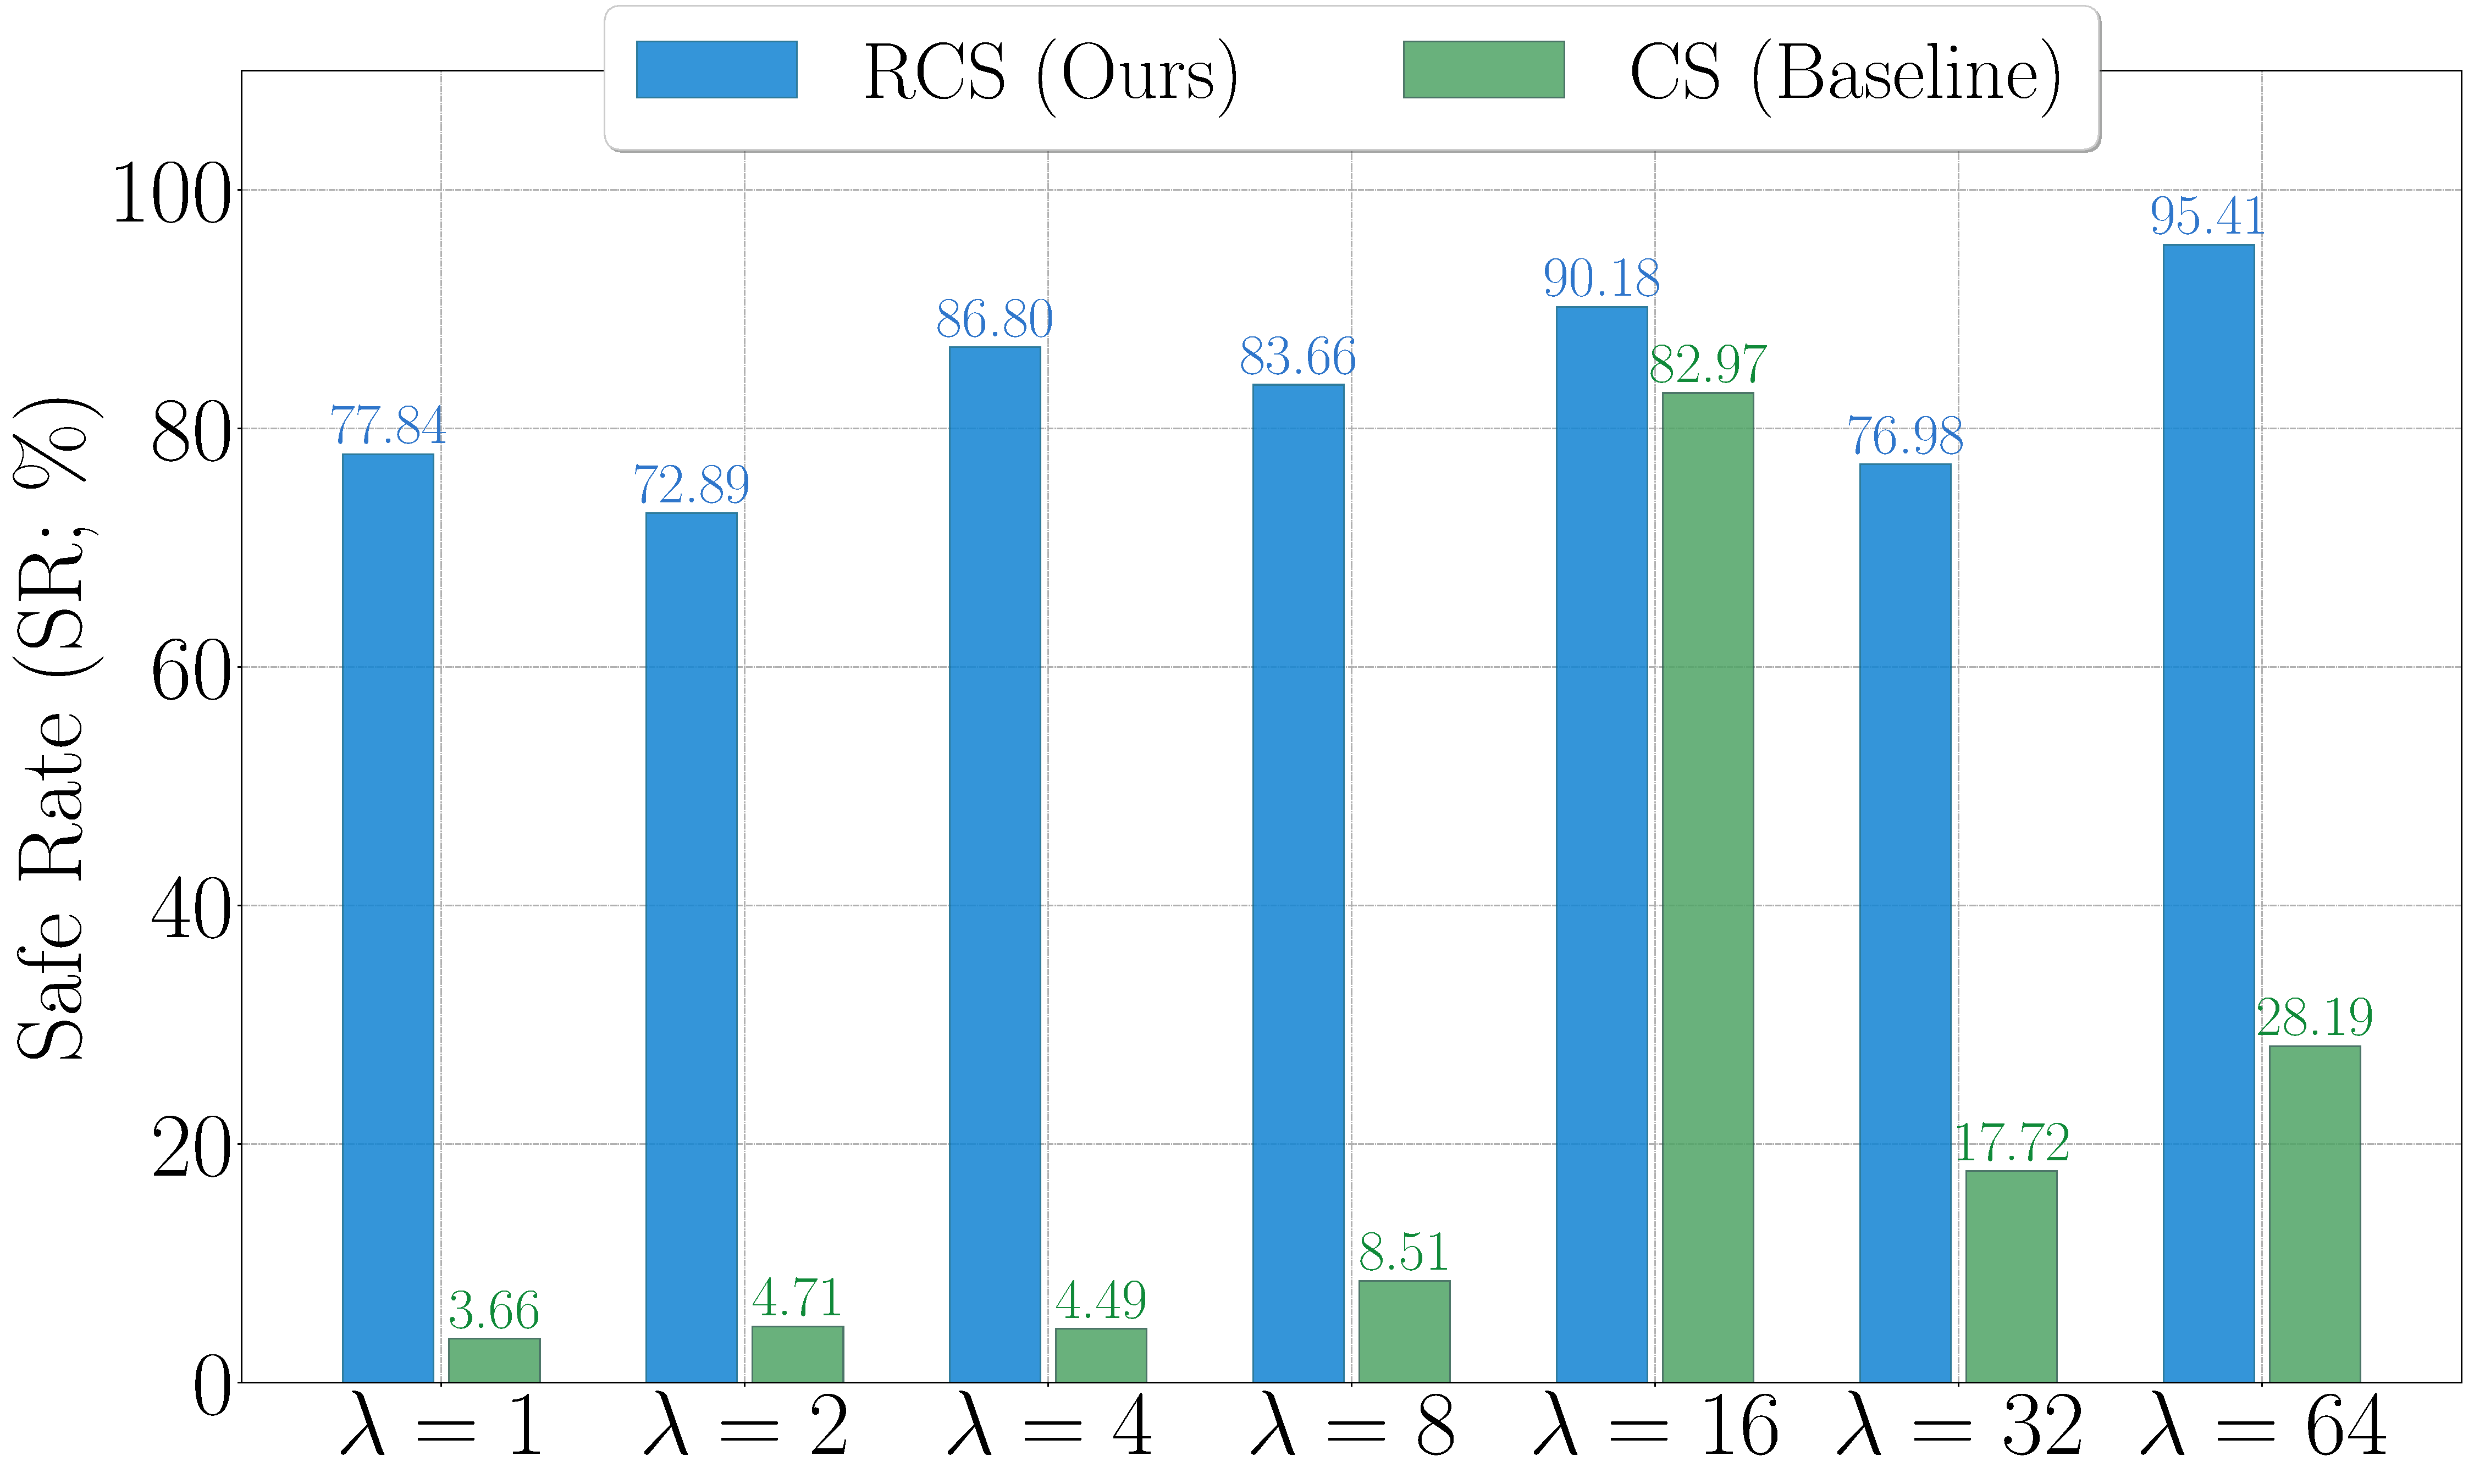
\includegraphics[width=\linewidth]{latex/eval_res_d/SR-66.pdf}
        \caption{$n=66$.}
    \end{subfigure}
    \begin{subfigure}{0.35\textwidth}
        \centering
        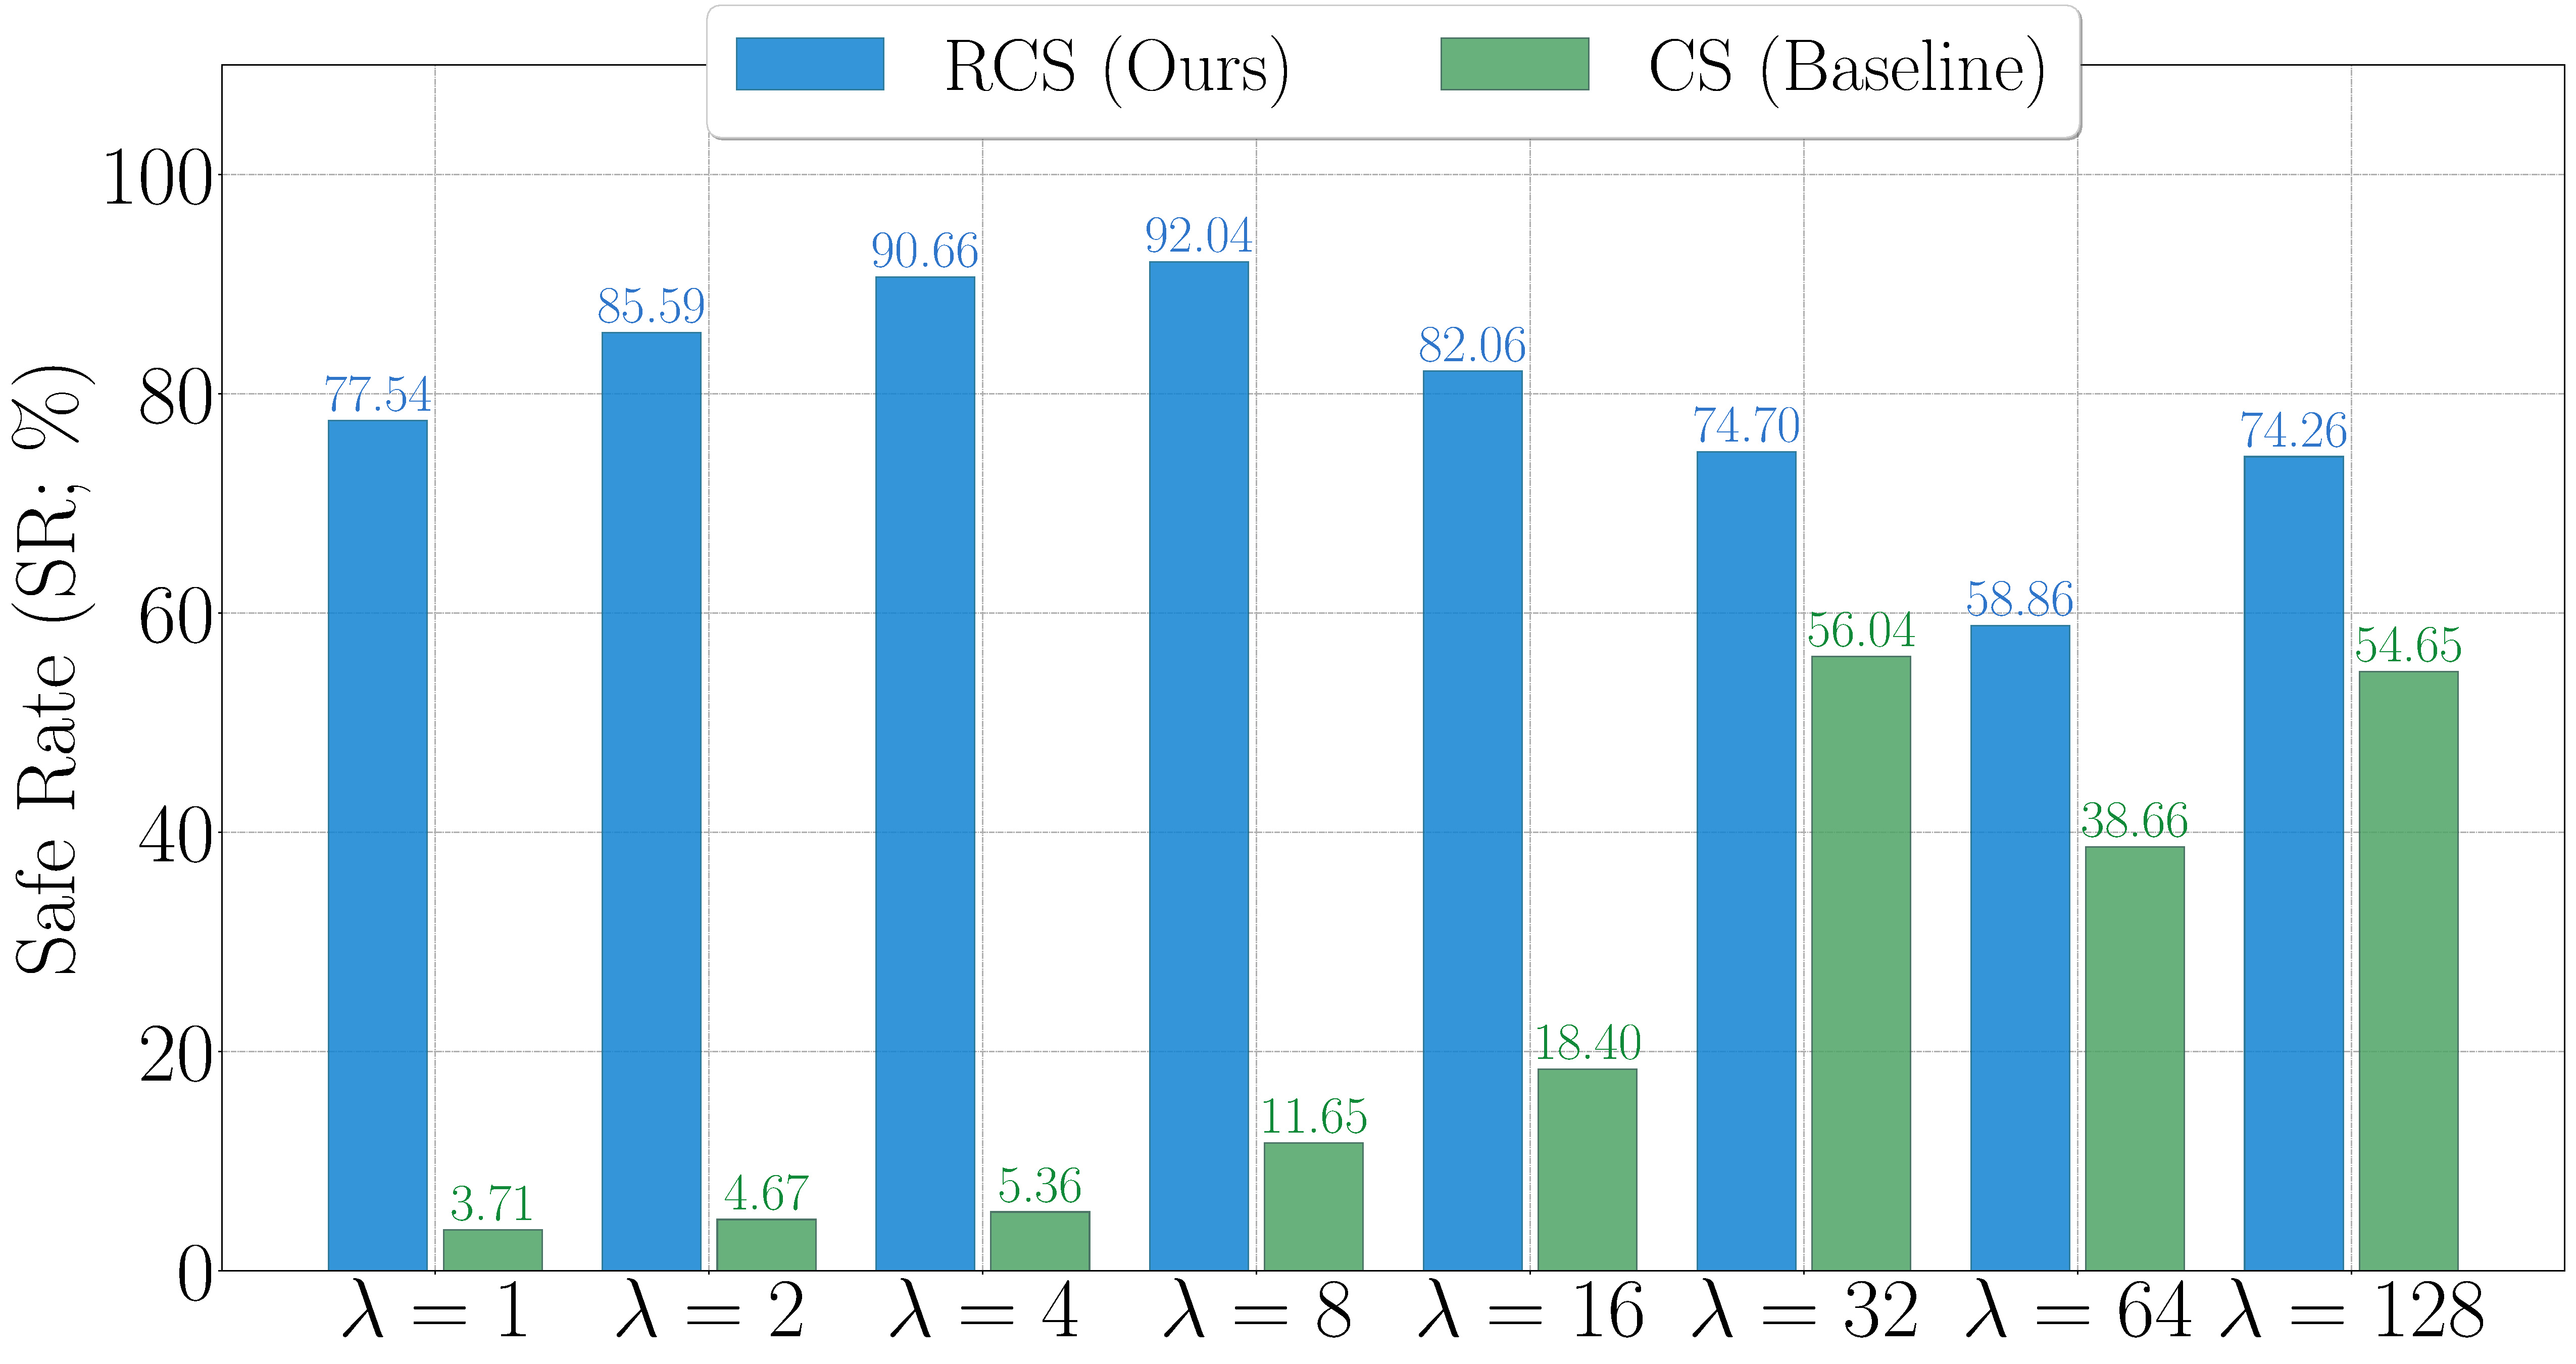
\includegraphics[width=\linewidth]{latex/eval_res_d/SR-130.pdf}
        \caption{$n=130$.}
    \end{subfigure}
    \caption{Evaluation results for the safe rate when $f = \lceil \frac{n}{2} \rceil$.}
    \label{fig:SR_d_app}
    % \vspace{-15pt}
\end{figure*}



\begin{figure*}[!]
    \centering
    \begin{subfigure}{0.31\textwidth}
        \centering
        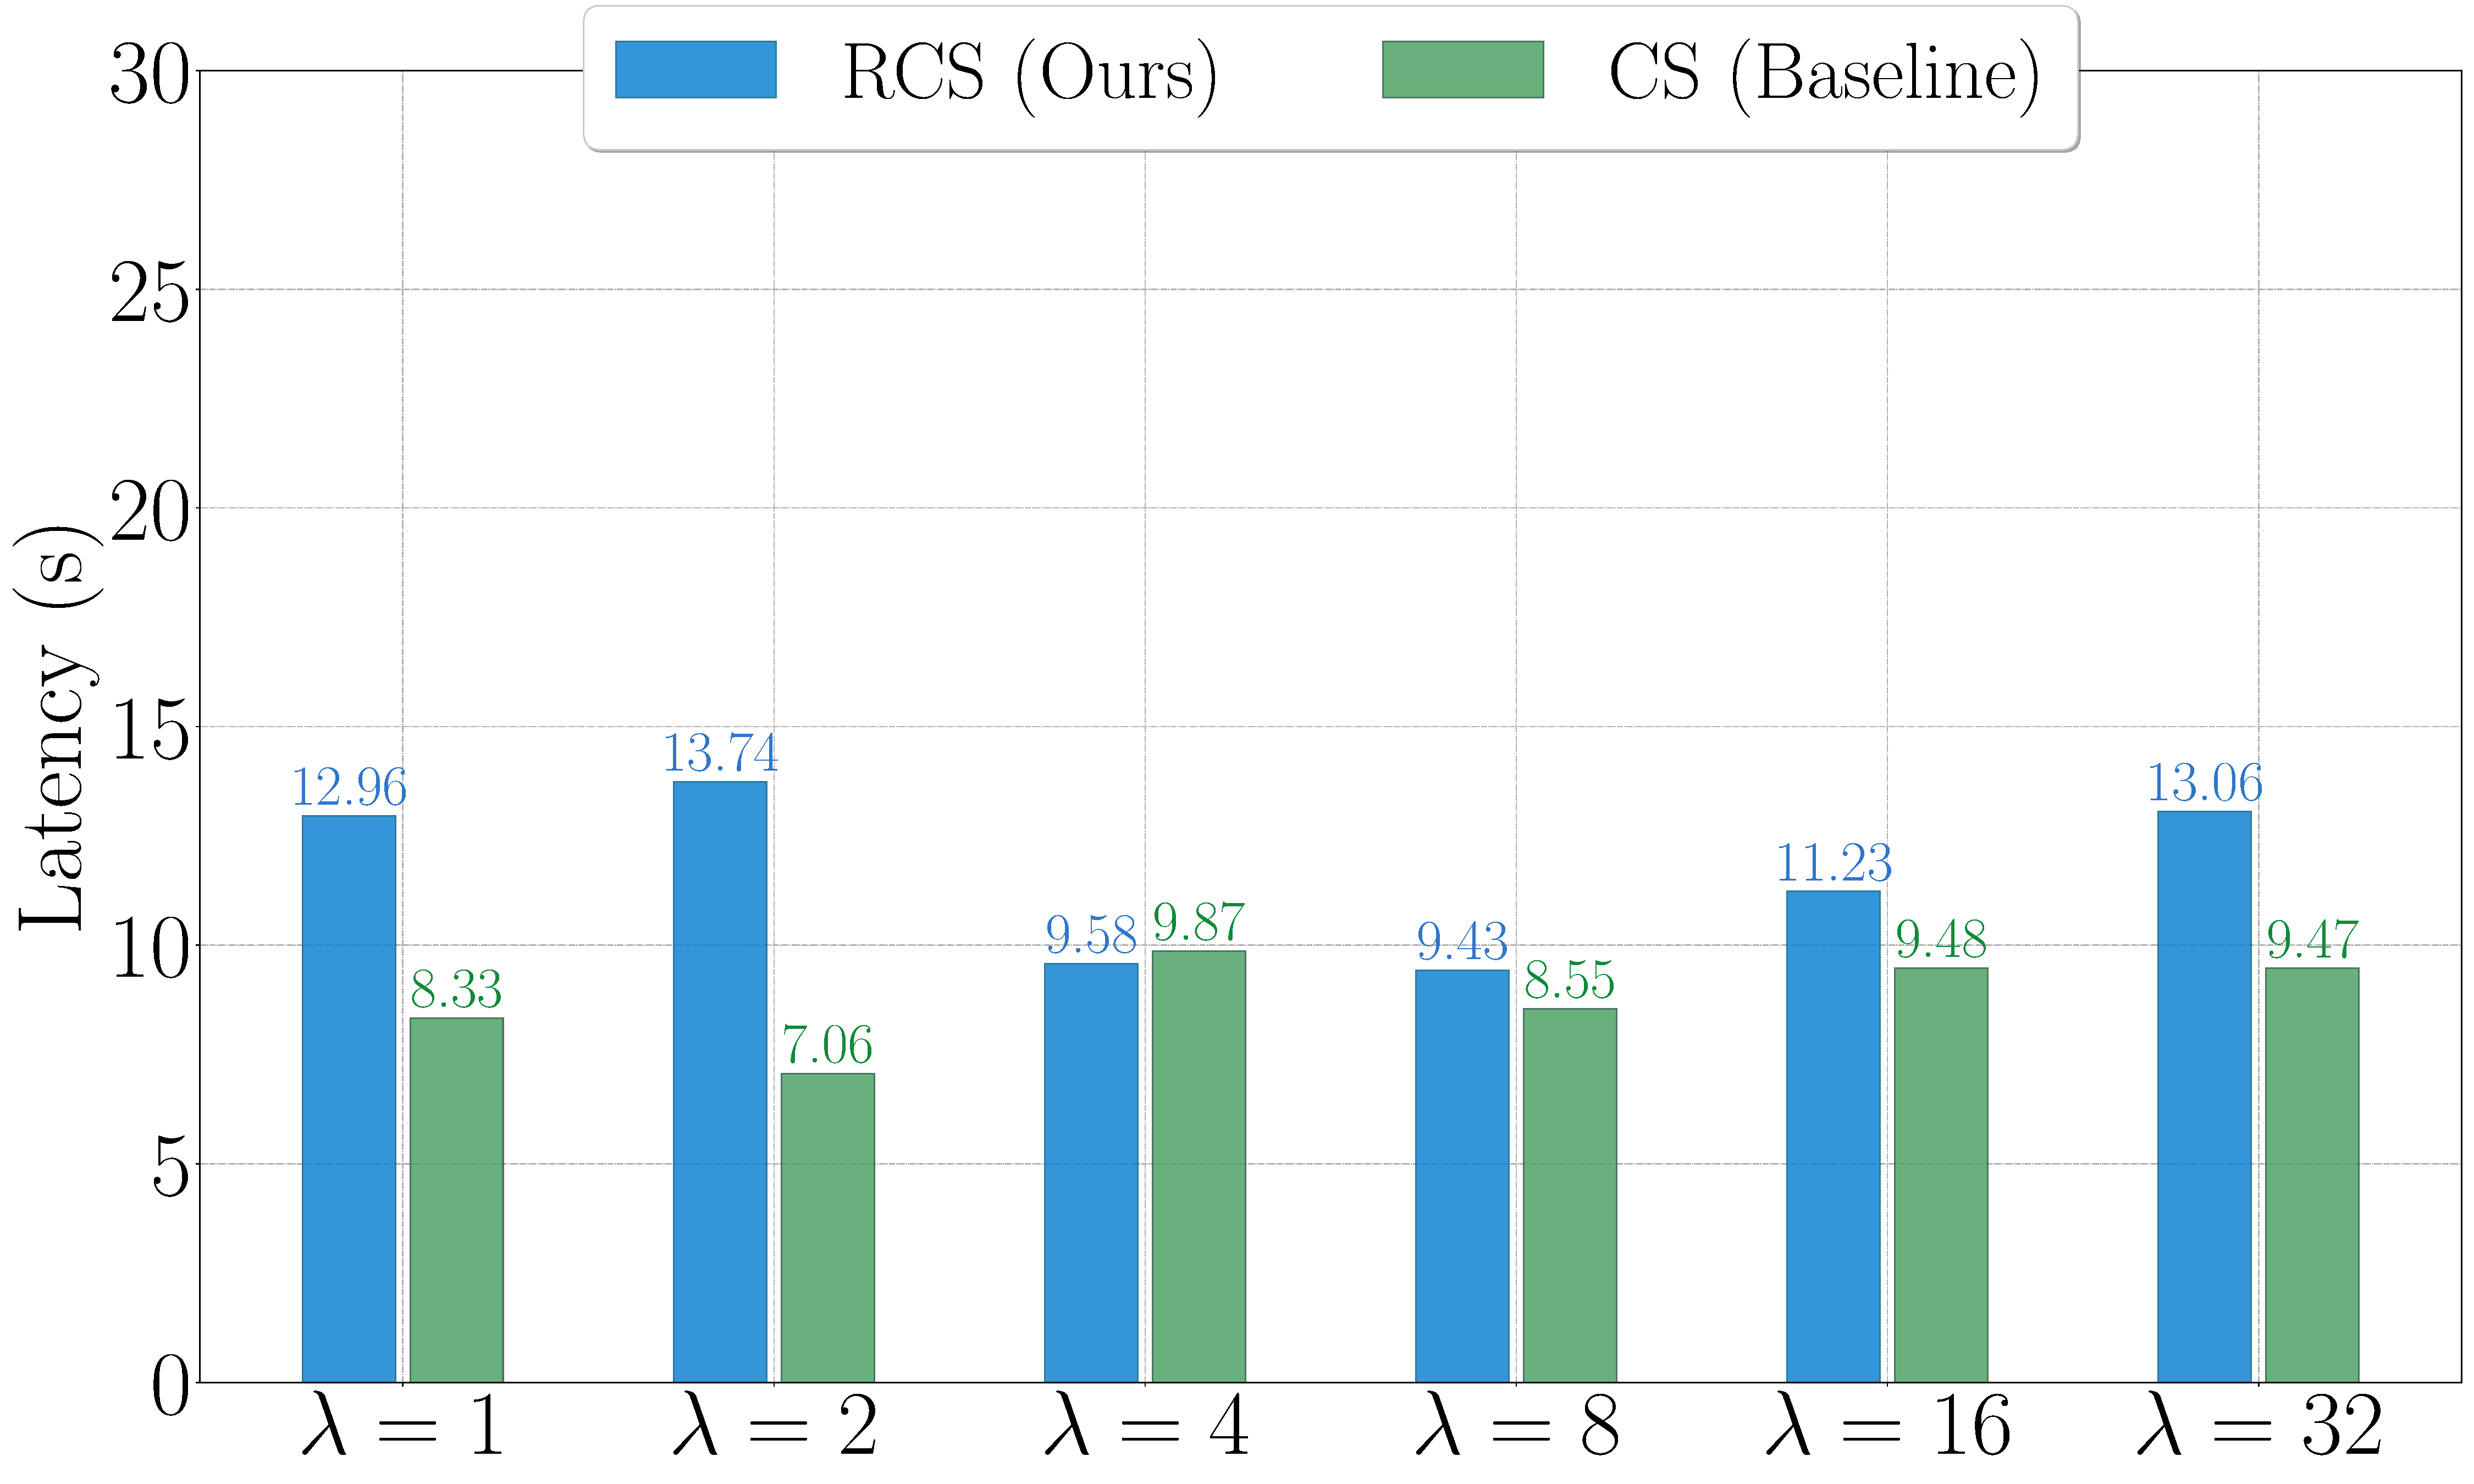
\includegraphics[width=\linewidth]{latex/eval_res_d/TC-34.pdf}
        \caption{$n=34$.}
    \end{subfigure}
    \begin{subfigure}{0.31\textwidth}
        \centering
        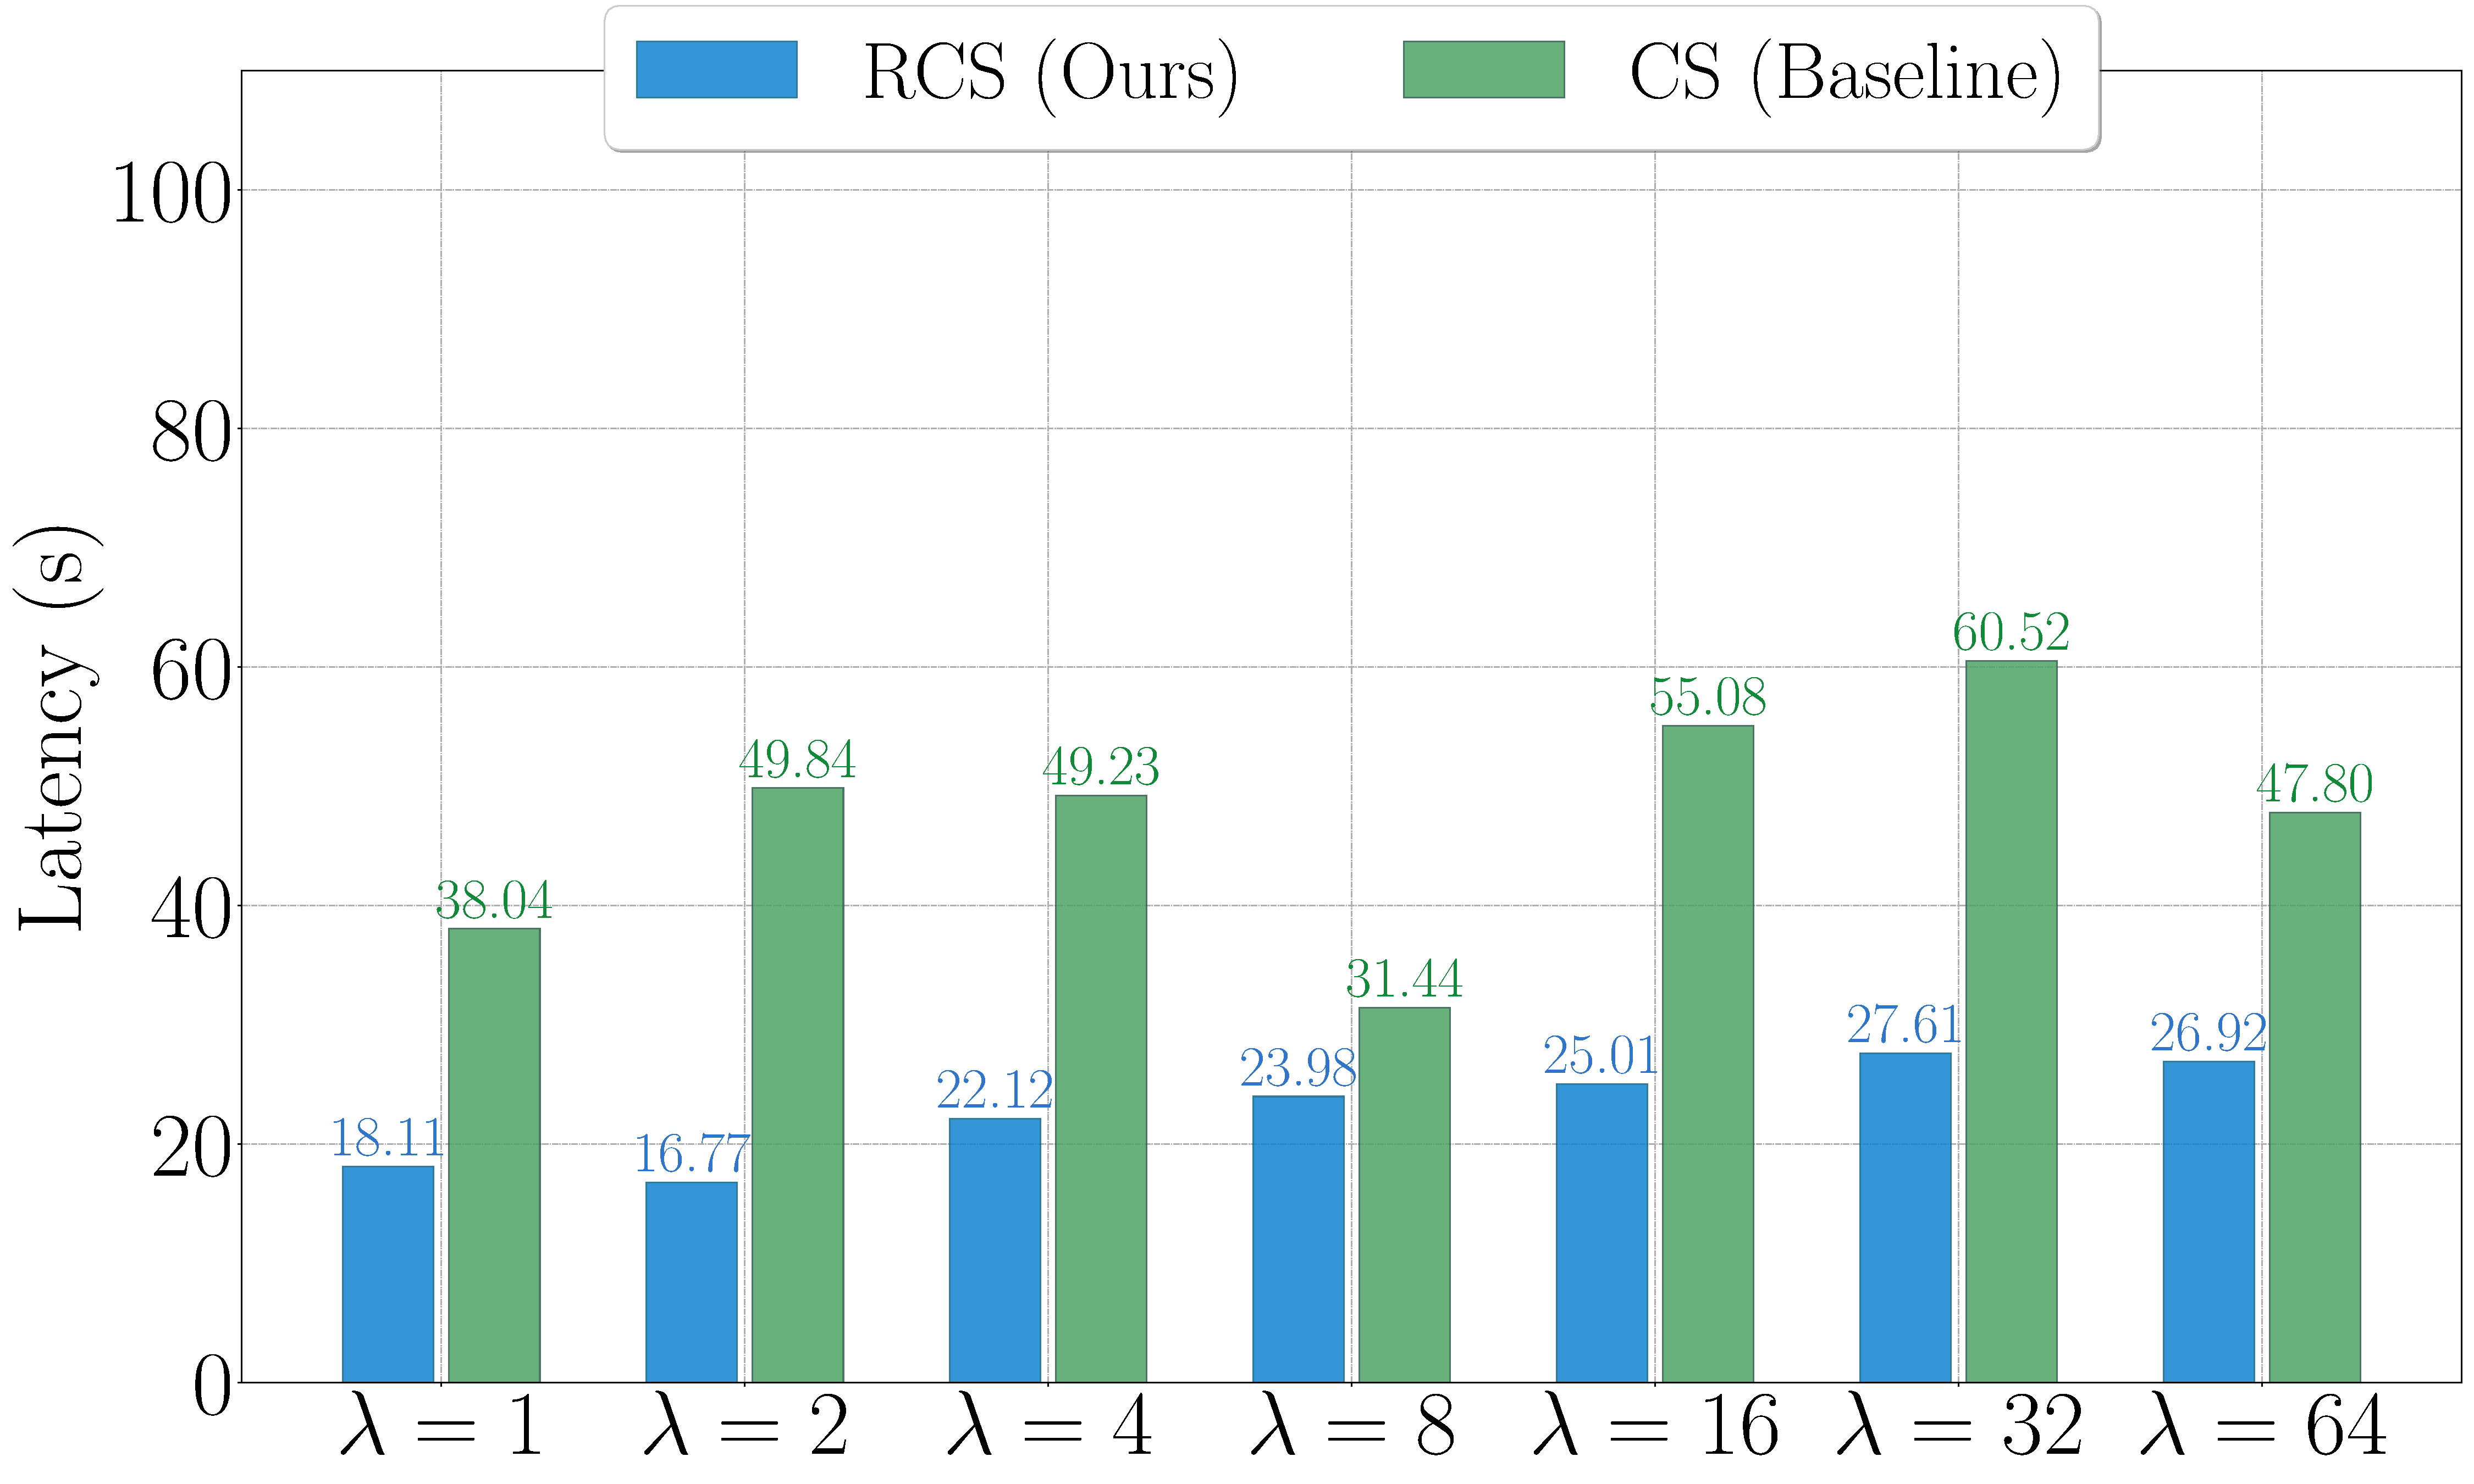
\includegraphics[width=\linewidth]{latex/eval_res_d/TC-66.pdf}
        \caption{$n=66$.}
    \end{subfigure}
    \begin{subfigure}{0.35\textwidth}
        \centering
        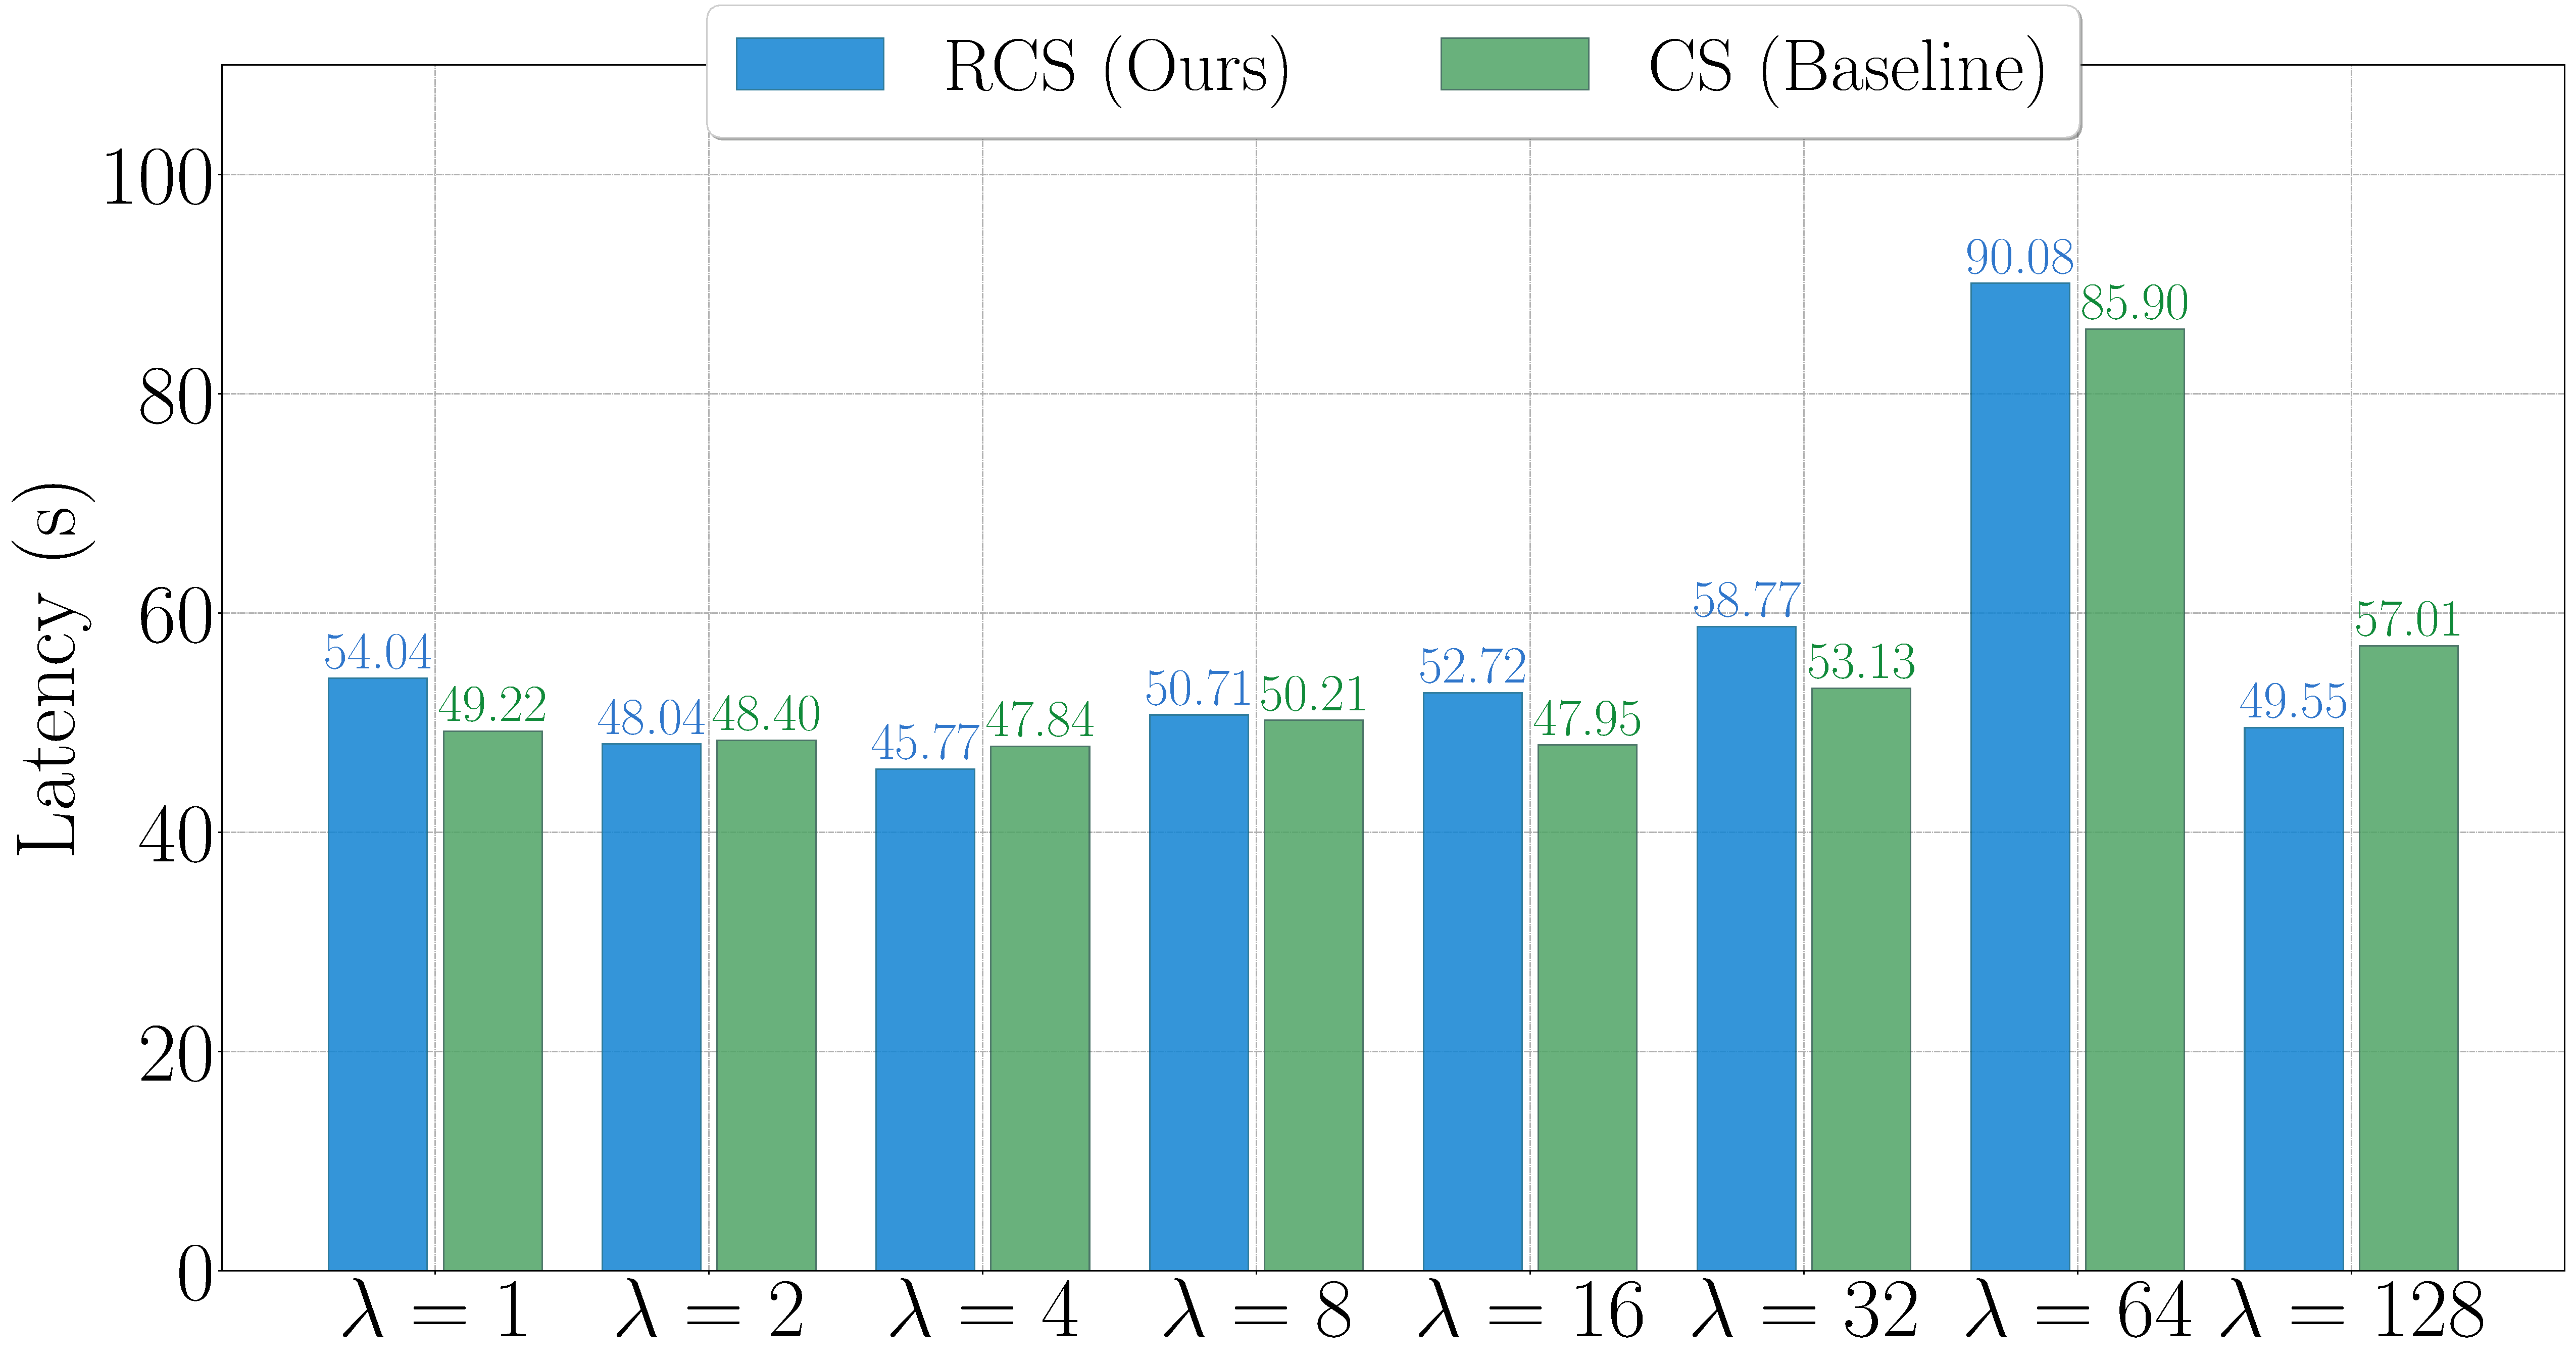
\includegraphics[width=\linewidth]{latex/eval_res_d/TC-130.pdf}
        \caption{$n=130$.}
    \end{subfigure}
    \caption{Evaluation results for the latency when $f = \lceil \frac{n}{2} \rceil$.}
    \label{fig:TC_d_app}
    % \vspace{-15pt}
\end{figure*}

\begin{figure}[!]
    \centering
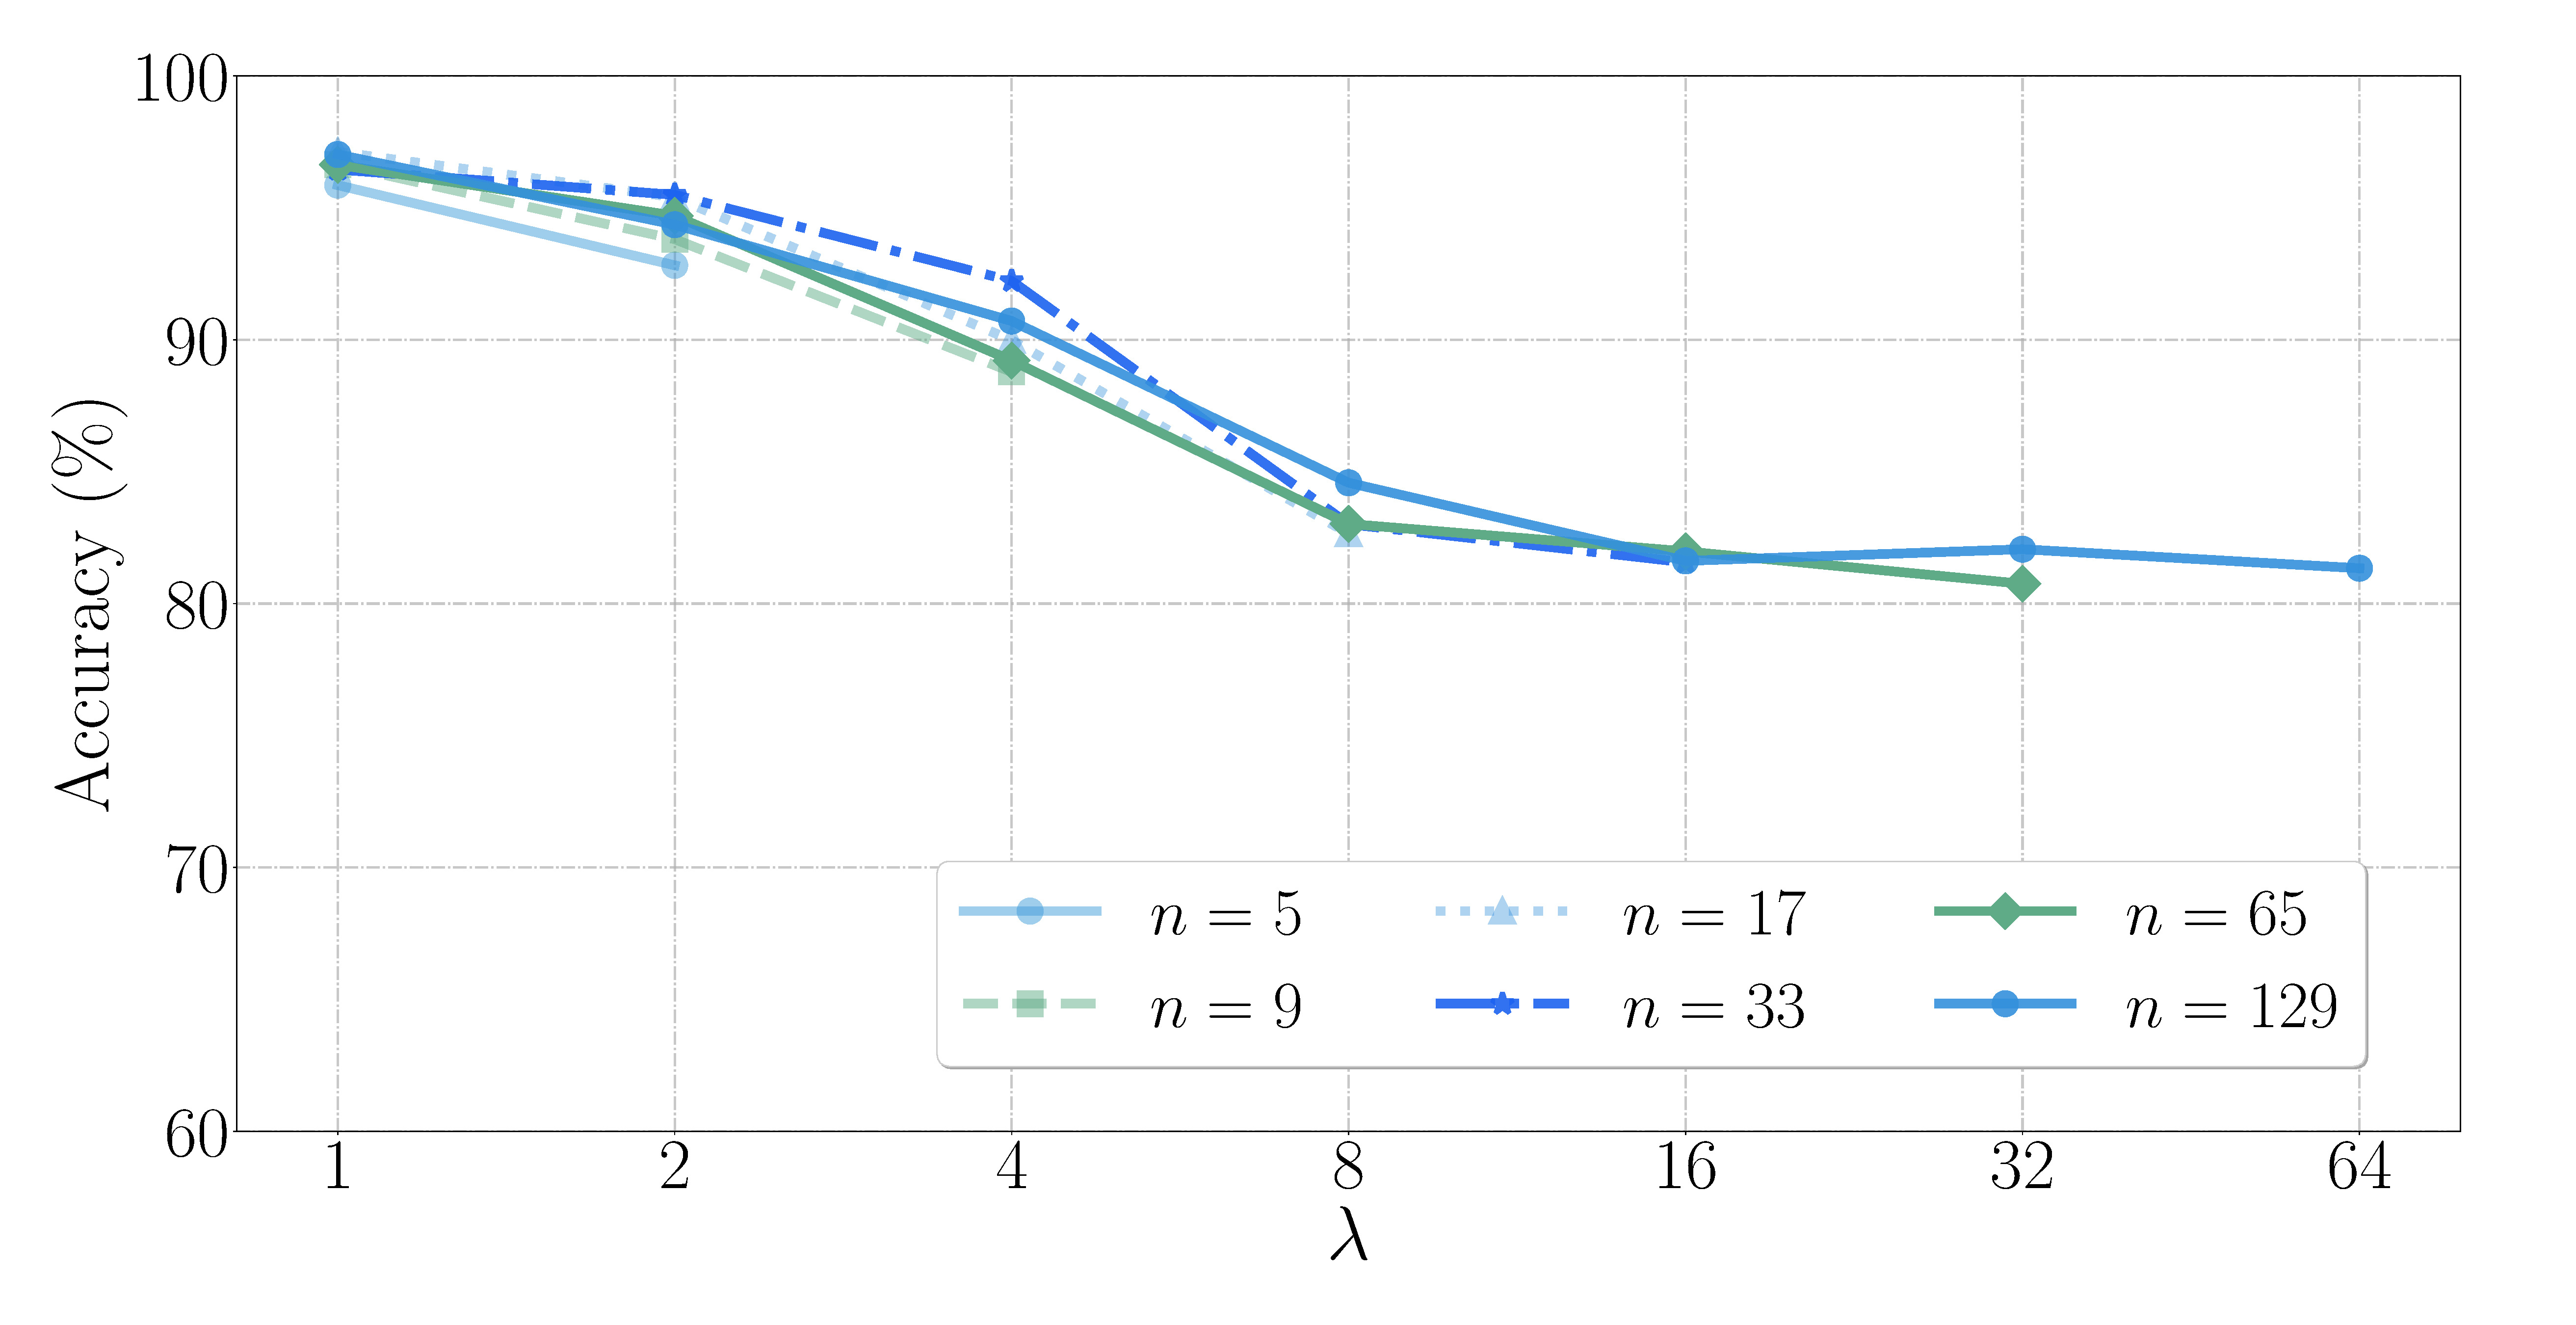
\includegraphics[width=0.56\linewidth]{latex/eval/DR_m.pdf}
    \caption{Accuracy of the feedback algorithm for different $\lambda$ and $n$ values when Byzantine models collude.}
    \label{fig:dr_m}   
    \vspace{-15pt}
\end{figure}

\section{Necessity Analysis of Liveness}
We further analyze the necessity of the liveness property. In real-world deployments, the goal of $\mathcal{MG}$ is not only to guarantee safety, but also to accomplish normal inference tasks such as mathematics, medical diagnosis, and programming. The objective is to maintain both functionality and safety, rather than prioritize safety as the sole consideration. As a result, in practical applications, $\mathcal{MG}$ must be able to perform valid reasoning on a wide variety of prompts. From the perspective of safety, abstention can be used to avoid unsafe responses. However, for regular inference tasks, abstention is not acceptable, as the response $\bot$ cannot adaptively provide reasonable outputs for unknown prompts. Therefore, liveness is necessary for $\mathcal{MG}$ from a practical application perspective. 